\documentclass[10pt]{article}
\usepackage{../../local}
\usepackage{listings}
\lstdefinestyle{tt}{basicstyle=\small\ttfamily,keywordstyle=\bfseries,language=[LaTeX]{TeX}}



\newcommand{\classcode}{CS 170}
\newcommand{\classname}{Efficient Algorithms and Intractable Problems}
\renewcommand{\maketitle}{%
\hrule height4pt
\large{Eric Du \hfill \classcode}
\newline
\large{Notes} \Large{\hfill \classname \hfill} \large{\today}
\hrule height4pt \vskip .7em
\small{Header styling inspired by CS 70: \url{https://www.eecs70.org/}}
\normalsize
}
\linespread{1.1}

\newcommand{\pre}{\mathrm{pre}}
\newcommand{\prev}{\mathrm{prev}}
\newcommand{\post}{\mathrm{post}}
\newcommand{\dist}{\mathrm{dist}}
\newcommand{\cost}{\mathrm{cost}}
\newcommand{\size}{\mathrm{size}}
\newcommand{\capacity}{\mathrm{capacity}}
\newcommand{\Var}{\mathrm{Var}}
\newcommand{\len}{\mathrm{len}}

%\newcommand{\question}[1]{\textcolor{red}{#1}}
%\newcommand{\answer}[1]{\textcolor{green!80!black!}{#1}}
%\renewcommand{\comment}[1]{\textcolor{blue!50}{#1}}
\begin{document}
	\maketitle
	\section{Introduction}
\subsection{Motivations} 
\begin{itemize}
	\item Why study this class?
		\begin{itemize}
			\item Given a "black box" circuit, with input and output leads, we can determine what's within 
				the "black 
				box".
			\item In this particular case, if our black box contains a voltage divider, and the output voltage is given 
				by the equation:
				\[
				v_{\text{out}}(t) = \frac{R_2}{R_1+ R_2}v_{\text{in}}(t)
				\] 
				In principle though, the signal can be anything that we want: for facial recognition software, the input
				signal could be the configuration of the intensity the camera picks up. There's many more we went over, 
				don't really want to write it all down. 
		\end{itemize}
	\item In essence, there's a lot of systems that can be modeled by a system that takes in a signal \( x(t) \), and 
		outputs a signal \( y(t) = f(x(t))\).
		\begin{itemize}
			\item The signals are usually functions of time, location, in any number of dimensions.
			\item The systems does some sort of transformation on an input signal. In particular, we will study 
				linear systems, shift-invariant systems, etc.
				
				We'll talk about mathematical operations that we use to perform these transformations: Fourier, 
				Laplace, Z-transformations, convolutions, correlation, etc.\item 
	\end{itemize}
\end{itemize}
\subsection{Types of Signals}
\begin{itemize}
	\item \textbf{Continuous-time:} signals defined over continuous variables (e.g. position, time). For 
		instance, a signal \( x(t) \) is continuous for our purposes, since time is a continuous variable. 

		Further, because \( t \) is continuous, then \( x \) must also be continuous.  If the signal is differentiable, 
		then the derivative \( \dv{x(t)}{t} \) also exists. 

		\question{\( t \) being continuous does not imply that \( x(t) \) is continuous (e.g. Thomae function),
		but is it true for this class?} 
	\item \textbf{Discrete-Time:} These are signals defined over discrete variables. For instance, if we had 
		\( x[n] \) as a signal, where \( n \) is an integer. 

		We don't have a concept of differentiability, but we can compute the difference: \( x[n] - x[n- 1] \), and 
		talk about that quantity. 
	\item \textbf{Real-Valued:} A signal \( x(t) \) is real-valued if \( x(t) \in \mathbb R \), where \( \mathbb R \) 
		denotes the set of all real numbers. 
	\item \textbf{Complex-Valued:} A signal \( x(t)  \) is complex-valued if \( x(t) \in \mathbb C \), where 
		\( \mathbb C \) denotes the set of complex numbers. 
	\item Note that while we're using the continuous-time notation here, the same concepts apply with discrete-time 
		signals. 

		\begin{itemize}
			\item Quick recap on complex numbers: denoted by \( a + bj \) or \( a + bi \), where \( i \) and \( j \) 
				denote the imaginary unit. 
			\item They are defined as \( i^2 = -1 \) or \( j^2 = -1 \).
			\item \( a \) is the real part, and \( b \) is the imaginary part. 
			\item We can plot these values in the complex plane, using the real and imaginary representation:
				\begin{center}
					\begin{tikzpicture}
						\draw[-stealth, thick] (-3, 0) -- (3, 0) node[above] {real};
						\draw[-stealth, thick] (0, -3) -- (0, 3) node[above right] {imaginary};
						\draw[red] (0, 0) -- (1.8, 1.4) node[above right, black] 
							{\( z = a + bj \) }; 
						\filldraw[red] (1.8, 1.4) circle (2pt); 
						\draw[dashed] (1.8, 1.4) -- (1.8, 0) node[below] {\( a \) };
						\draw[dashed] (1.8, 1.4) -- (0, 1.4) node[left] {\( b \) };
					\end{tikzpicture}
				\end{center}
				Or using the magnitude-phase representation:
				\begin{center}
					\begin{tikzpicture}
						\draw[-stealth, thick] (-3, 0) -- (3, 0) node[above] {real};
						\draw[-stealth, thick] (0, -3) -- (0, 3) node[above right] {imaginary};
						\draw[red] (0, 0) -- node[midway, above left] {\( m \) } (1.8, 1.4) node[above right, black] 
							{\( z = m\cdot e^{j \theta} \) }; 
						\filldraw[red] (1.8, 1.4) circle (2pt); 
						\draw[red] (1, 0) arc (0:37.87:1) node[midway, right]{\( \theta \) };
						\draw[dashed] (1.8, 1.4) -- (1.8, 0) node[below] {\( m \cdot \cos (\theta) \) };
						\draw[dashed] (1.8, 1.4) -- (0, 1.4) node[left] {\( m \cdot \sin (\theta) \) };
					\end{tikzpicture}
				\end{center}
				We represent the magnitude as \( m = |z| \), and the phase angle \( \theta \) is the angle made 
				with the real axis. 
		\end{itemize}
	\item \textbf{Periodic Signal:} Two quantities we'll introduce here: the period \( T \) is the time it takes 
		for the signal to repeat itself. \( T \) is measured in units of time, generally seconds.
		
		The frequency \( f \) is the "inverse" of period, defined by \( f = \frac{1}{T} \). We will also use 
		the angular frequency \( \omega \), defined by \( \omega = \frac{2\pi}{T} = 2 \pi f \). Angular frequency
		is mainly going to be used when we involve complex numbers. We will see:
		\[
		e^{j \omega t} = e^{j (2 \pi f t)} = \cos(2 \pi ft) + i \sin (2 \pi ft)
		\] 
	\item \textbf{Dimensionality:} We will deal with multi-dimensional signals: an example of a 2D signal are images, 
		which determine the color of a pixel based on a row and column. The spaces that we'll be working with are 
		either \( \mathbb R^{n} \) or \( \mathbb C^{n} \). 
\end{itemize}
\subsection{Signal Transformations}
\begin{itemize}
	\item \textbf{Shifts:} Essentially just shifts the signal along one dimension: \( x(t) \to x(t - T) \). \( T \) 
		is some constant. If  \( T > 0 \), then the shift is to the \textit{right}, and if \( T < 0 \) then 
		the shift is to the \textit{left}.
	\item \textbf{Scaling:} We can multiply a signal \( x(t)  \) by some constant \( a \) : \( x(t) \to a\cdot x(t) \).
		If \( a < 1 \), then we shrink \( x(t) \), and if \(  a > 1 \) then we amplify the signal. 
	\item \textbf{Reversal:} Given \( x(t) \), we can "reverse time" by adding a negative to the argument: \( x(t)
		\to x(-t)\). Visually, all we do is flip the signal around the \( y \)-axis.  
\end{itemize}
\subsection{Signal Properties}
\begin{itemize}
	\item \textbf{Even:} Functions which satisfy \( x(t) = x(-t) \). In other words, if we perform a reversal, the 
		signal stays the same.
	\item \textbf{Odd:} Functions which satisfy \( x(t) = -x(-t) \). If we perform a reversal, the signal becomes the 
		negative of itself.
	\item \textbf{Periodic:} If \( T \) is the period, then \( nT \) is also a period for any \( n \in \mathbb Z \).
		However, we will call \( T \) the fundamental period; the smallest \( T \) for which the function 
		repeats. 

		For the function \( \sin(2 \pi ft) \), the fundamental period is \( 1 / f \).  
\end{itemize}
\subsection{Model Functions}
\begin{itemize}
	\item These are called model functions because they're idealized models to analyze. 
	\item \textbf{Heaviside Step function:} For the continuous-time case it's usually modeled by:
		\[
		u(t) = \begin{cases}
			0 & \text{for \( t < 0 \)}\\
			1 & \text{for \( t \ge 0 \)}
		\end{cases}
		\] 
		In the discrete-time case, it's written as:
		\[
			u[n] = \begin{cases}
				0 & \text{for \( n < 0 \)}\\
				1 & \text{for \(n \ge  0\)}
			\end{cases}
		\] 
\end{itemize}




	%\section{More on Model Functions, System Characterization}
\section{Lecture 2}
\subsection{Model Functions Continued}
\begin{itemize}
	\item \textbf{Ramp Function:} The continuous-time is expressed as:
		\[
		r(t) = \begin{cases}
			0 & \text{for \( t < 0 \)}\\
			t & \text{for \( t \ge 0 \)}
		\end{cases}
		\] 
		Similarly in discrete time:
		\[
			\text{ramp}[n] = \begin{cases}
				0 & \text{for \( n < 0 \)}\\
				n & \text{for \( n \ge 0 \)}
			\end{cases}
		\] 
		Note that we can express the ramp function in terms of the step function, in many ways:
		\begin{itemize}
			\item \( r(t) = t \cdot u(t) \)
			\item \( r(t) = \int_{-\infty}^{t}u(t) \diff t \), the discrete case is just a sum over the same bound.
		\end{itemize}
	\item \textbf{Rectangular Function:} In continuous-time:
		\[
		\text{rect}(t) = \sqcap(t) = \begin{cases}
			1 & \text{for \( |t| \le  1 / 2 \)}\\
			0 & \text{else}
		\end{cases}
		\] 
		In discrete time:
		\[
		\text{rect}\left[ \frac{n}{N} \right] = \begin{cases}
			1 & \text{for \( |n| \le  N \)}\\
			0 & \text{for \( |n| > N \)}
		\end{cases}
		\] 
		We can also express \( \text{rect}(t) \) in terms of \( u(t) \) :
		\[
			\sqcap(t) = u\left( t + \frac{T}{2} \right)	- u\left( t - \frac{T}{2} \right) 
		\] 
	\item \textbf{Triangle Function:} In continuous-time:
		\[
		\Lambda(t) = \begin{cases}
			1 - |t| & \text{for \( |t| \le  1 \)}\\
			0 & \text{for \( |t| > 1 \)}
		\end{cases}
		\] 
		And in discrete-time:
		\[
		\Lambda \left[ \frac{n}{N} \right]  = \begin{cases}
			1 - \left|\frac{n}{N}\right| & \text{for \( |n| \le N \)}\\
			0 &\text{else}
		\end{cases}
		\] 
	\item \textbf{Delta Function:} In continuous time, it's called the Dirac delta function. It has the property 
		that \( \delta(t) = 0 \) for all \( t \neq 0  \), but 
		\[
		\int_{-\infty}^{\infty} \delta(t) \diff t  = 1
		\] 
		So in essence, this is an infinitesimally "thin" function, that extends to infinity. There are also 
		other ways to represent the Delta function:
		\begin{itemize}
			\item Derivative of the Heaviside step function: \( \delta(t) = \dv{u(t)}{t} \)
			\item The integral of a complex exponential:
				\[
				\delta(t) = \int_{-\infty}^{\infty} e^{j 2 \pi f t} \diff f = \frac{1}{2\pi}
				\int_{-\infty}^{\infty} e^{j \omega t}\diff  \omega 
				\] 
				\comment{The delta function allows us to approximate the integral \( \int_{-\infty}^{\infty} \cos(\omega t)
				\diff  t\). We can do the following:
				\begin{align*}
					\int_{-\infty}^{\infty} \cos(\omega t) \diff t &= \Re\left[ \int_{-\infty}^{\infty} \cos(\omega t) + 
					i \sin (\omega t)\right] \diff t \\
					&= \Re\left[ \int_{-\infty}^{\infty} e^{i \omega t} \diff  t  \right]  \\
					&= \Re\left[ 2\pi \delta(\omega)  \right]  
				\end{align*}
				Looking at the delta function, we know that when \( \omega = 0 \), then \( \cos(\omega t) = 1 \), so
				the integral diverges, as expected. When \(  \omega \neq 0  \), our integral result implies that 
				the integral evaluates to 0. This is not exactly true since the integral will oscillate 
				between \( \pm 1 \), which is relatively small compared to \( \omega = 0 \), so it can effectively 
				be taken as 0.}
		\end{itemize}
		\question{How does this compare with the definition we use in physics that \( \delta(t) \) is defined as 
			the function which satisfies:
			\[
			\int_{-\infty}^{\infty} f(t) \delta(t) = f(0) 
			\] 
		Do both work?} 

		\answer{See below bullet point, the definition allows you to derive this property.} 
	\item Let's explore some properties of the Delta function: 
		\begin{itemize}
			\item \textbf{Scaling:} 
				\[
					\int_{-\infty}^{\infty} \delta(\alpha t) dt = \int_{-\infty}^{\infty} \delta(t) \dv{\tau}{\alpha}
					= \frac{1}{|\alpha|}
				\] 
				In other words, \( \delta(\alpha t) = \frac{\delta(t)}{|\alpha|} \)
			\item \textbf{Sifting:} If we have \( f(t) \) and multiply it by a Delta function:
				\[
				\int_{-\infty}^{\infty} f(t) \delta(t - T) \diff t = f(T) 
				\] 
			\item \textbf{Delta function of a function:} We can take the delta function of a function as well:
				\[
				\delta(f(t)) = \frac{\delta(t - t_0)}{|f'(t_0)|}, \ f(t_0) = 0
				\] 
				We take the derivative in the denominator. 
		\end{itemize}
	\item In discrete time, the delta function is represented as the Kronecker delta:
		\[
			\delta[n] = \begin{cases}
				1 & n = 0\\
				0 & \text{else}
			\end{cases}
		\] 
		The function attempts to model the Dirac delta but for discrete time intervals:
		\[
			\sum_{n =-\infty}^{\infty}x[n] \delta[n - 10] = x[10]
		\] 
	\item \textbf{Shah function:} It's basically a bunch of Dirac deltas:
		\[
			\text{III}(t) = \sum_{k= 0}^{\infty}\delta(t - k)
		\] 
		In discrete time, it also is a sum of all deltas:
		\[
			\text{III}[n] = \sum_{k = 0}^{\infty}\delta[n - k]
		\] 
\end{itemize}
\subsection{System Characterization} 
\begin{itemize}
	\item Systems perform operations on input signals, like functions \( F: x \to y \). For instance, 
		the following is a moving average filter:
		\[
			y[n] = \frac{1}{3}(x[n - 1] + x[n] + x[n + 1])
		\] 
	\item We will be particularly interested in \textbf{linear systems}, systems which satisfy the following 
		two properties:
		\begin{itemize}
			\item \textbf{Scaling:} If for any input-output pair \( x(t) \to y(t) \), then for any constant \( a \), 
				\( ax(t) \to ay(t) \)
			\item \textbf{Addition:} Given any two input-output pairs 
				\begin{align*}
					x_1(t) &\to y_1(t)\\
					x_2(t) &\to y_2(t)
				\end{align*}
				Then it's also true that \( x_1(t) + x_2(t) \to y_1(t) + y_2(t) \)
		\end{itemize}
		Combining these two properties, given two general signals \( x_1(t) \to y_1(t) \) and \( x_2(t) \to y_2(t) \), 
		then \( ax_1(t) + bx_2(t) \to ay_1(t) + by_2(t)\).

		\comment{Note that a function like \( y(t) = x(t) + b \) is not a linear function, becuase it doesn't 
			satisfy the second property. Even though the function is linear, doesn't mean that the transformation 
		is linear.} 
	\item \textbf{Shift Invariant:} A shift-invariant system is a system where if we shift the input, the output 
		is also shifted. Given \( x(t) \) and its output \( y(t) \), then \( x(t - T) \) should produce 
		 \( y(t -T) \) for any \( T \).
	 \item \textbf{Memoryless:} A function whose output at any given time only depends on the input at that 
		 time. For instance, machine learning algorithms are not memoryless, since their output depends on 
		 previous inputs. 

		 \question{Does "current" here refer to a given input, or does it refer to past inputs? For instance, 
		 is the moving average function considered memoryless?}

		 Most systems that take time to react are not considered memoryless, since 
	 \item \textbf{Causality:} A system is causal if the output depends on the input at the present and past times 
		 only, not on future times. A system defined by:
		 \[
			 y[n] = \frac{1}{3} (x[n] + x[n + 1])
		 \] 
		 is not considered causal, because \( y[n] \) depends on the \( n + 1 \)-th input. 
	 \item \textbf{Stability:} There are many different ways to define stability, here are some of them:
		 \begin{itemize}
		 	\item A system is called BIBO stable if bounded inputs generate boudned 
		 outputs. Mathematically, this means:
		 \[
		 \int_{-\infty}^{\infty} |x(t)|\diff t  < \infty
		 \] 
		 And in discrete time:
		 \[
		 \sum_{-\infty}^\infty |x[n]| < \infty
		 \] 
	 \item We can also look at the energy and power:
		 \[
		 E = \int_{-\infty}^{\infty} |x(t)|^2 \diff t  \ \ P = \lim_{T \to \infty } \int_{-T / 2}^{T / 2} |x(t)|^2 
		 \diff t
		 \] 
		 \end{itemize} 
	 \item \textbf{System Response function:} These are particular outputs for systems when given an impulse 
		 response of a delta function. They are calculated by substituting \( x(t) = \delta(t)  \) in the 
		 continuous case, and \( x[n] = \delta[n] \) in the discrete case. 
		 \question{Watch lecture for this.}

		 To calculate the impulse response for the moving average filter:
		 \[
			 y[n] = \frac{1}{3}(x[n -1] + x[n] + x[n + 1])
		 \] 
		 To find the impulse response, we substitute \( x[n] = \delta[n] \) to get \( h[n] \). Here, notice that 
		 for \( n < -2 \), then \( h[n] = 0 \), since \( x[-2 + 1] = x[-1] = 0 \), and same goes for the other terms. 
		 Then, refer to the following table:
		 \begin{center}
			 \begin{tabular}{c|c}
				 \( n \) & \( h[n] \) \\
				 \hline 
				 -2 & 0 \\
				 -1 & 1/3\\
				 0 & 1/3\\
				 1 & 1/3\\
				 2 & 0
		 	\end{tabular}
		 \end{center}
\end{itemize}

	\section{Characterization Continued}
\subsection{Step Response}
\begin{itemize}
	\item The step response function is the function \( y_{\text{step}}(t) \) when a step function 
		\( u(t) \) is fed into the system. In discrete-time: we feed \( u[n] \) into the system, and get 
		\( y_{\text{step}}[n] \) as an output.
	\item For instance, for the moving average filter defined earlier, we have the following result:
		\begin{center}
			\begin{tabular}{c|c}
				\( n \) &  \( y_{\text{step}}[n] \)\\
				\hline 
				-2 & 0\\
				-1 & 1/3\\
				0 & 2/3\\
				1 & 1\\
				2 & 1
			\end{tabular}
		\end{center}
		Note that this resembles a ramp function, and is called a ramp-step function.
	\item \textbf{Harmonic Response:} The harmonic response is the response by the system when presented with 
		a harmonic function, of the form \( Ae^{i \omega t}\). 

		In discrete time, we feed in \( Ae^{i \omega n} \) where \( n \) is an integer. 
	\item For the moving average filter, let's write out \( y[n] \) :
		\begin{align*}
			y[n] &= \frac{1}{3}\left(Ae^{i \omega (n - 1)} + Ae^{i \omega n} + Ae^{i \omega (n + 1)}\right)\\
			&= \frac{1}{3}\left( e^{-i \omega} + 1 + e^{i \omega} \right)  \\
			&= \frac{1}{3}(2 \cos \omega + 1) Ae^{i \omega n} \\
		\end{align*}
		The interesting thing here is that when given a harmonic function, the system response just scales the signal 
		by a constant amount!
\end{itemize}
\subsection{LCCDE} 
\begin{itemize}
	\item In this class, we will deal with lots of differential equations, so it's going to be very useful to 
		look at their form, and how to solve them.   
	\item There are two solutions to any differential equation: 
		\begin{itemize}
			\item \textbf{Particular Solution:} \( y_p(t) \) is called a particular solution if it satisfies:
				\[
					\sum_{k = 0}^{N}a_k \dv[k]{y_p(t)}{t} = \sum_{k = 0}^{N}b_k \dv[k]{x(t)}{t}
				\] 
			\item \textbf{Homogeneous Solution:} \( y_h(t) \) is called a homogeneous solution if it satisfies:  
				\[
						\sum_{k = 0}^{N}a_k \dv[k]{y_p(t)}{t} =	0
				\] 
		\end{itemize}
	\item In general, the solution will be a linear combination of the two: 
		\[
		y(t) = y_p(T) + ay_h(t)
		\] 
		the value of \( a \) is generally going to be given by some initial condition. 
	\item For the homogeneous solution, an ansats of the form \( Ae^{st} \) where \( s \) is an undetermined constant 
		will solve the differental equation. We can then determine the value of \( s \) by solving the resulting 
		polynomial.

		To determine the value of \( A \), these are determined by the initial conditions, and depending on the 
		number of initial conditions given, that would correspond directly to the number of distinct values of \( A \). 
\end{itemize}


	%\section{Block Diagrams, Linearly Invariant Systems}
\section{Lecture 4}
\subsection{System Block Diagram}
\begin{itemize}
	\item Now we'll look at how to convert an LCCDE into a block diagram. 
	\item Suppose we're given a system of the form
		\[
			\sum_{k = 0}^{N}a_k y[n - k]  = \sum_{k = 0}^{M}b_k x[n - k]
		\] 
		This implies the equation:
		\[
			y[n] = \sum_{k = 0}^{M}\frac{b_k}{a_0}x[n - k] - \sum_{k = 1}^{N}\frac{a_k}{a_0}y[n - k]
		\] 
\end{itemize}
\subsection{Linear Time Invariant (LTI), Linear Shift Invariant (LSI)}
\begin{itemize}
	\item What is an LTI system? Firstly, it's linear, so it satisfies the superposition rule: given 
		two signals \( x_1(t) \) and \( x_2(t) \), then an input of \( ax_1(t) + bx_2(t) \) will generate 
		an output of \( ay_1(t) + by_2(t) \). 
	\item An LSI is also a linear system, and given an input signal \( x(t) \) with an output 
		\( y(t) \), then we can shift
		the system \( x(t - T) \) to generate an output \( y(t - T) \), but \( y(t - T) = y(t) \). In other words, 
		the output will look like \( y(t) \), except shifted by \( T \).  
	\item As an example, the continuous LCCDE is a linear time invariant system. This is because the derivative 
		is linear: 
		\[
			\sum_{k = 0}^{M}\dv[k]{(ax_1(t) + bx_2(t)}{t} = \sum_{k = 0}^{M}b_k \dv[k]{x(t - T)}{(t - T)}
		\] 
		And then we can substitute \( u = t - T \) :
		\[
			\sum_{k = 0}^{M}b_k \dv[k]{x(u)}{u} = \sum_{k = 0}^{M}\dv[k]{y(t - T)}{(t - T)}
		\] 
	\item The same principle also holds for discrete time signals. 
	\item The most important property of an LTI system is that \textbf{the system response is fully characterized 
		by an impulse response function.}

		What this means is that if we feed the system a \( \delta(t) \) or \( \delta[n] \), it gives us an 
		impulse response function \( h(t) \) or \( h[n] \), and this gives us enough information to characterize
		the entire system.
	\item In the continuous time case, suppose we had the following:
		\begin{center}
			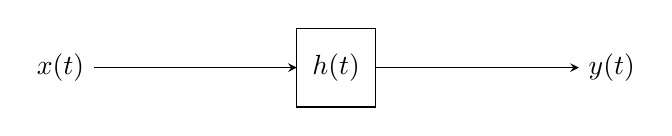
\begin{tikzpicture}
				\node (A) at (-3, 0) {\( x(t) \) };
				\node (B) at (4, 0) {\( y(t) \) };
				\draw[-stealth] (A) -- (0, 0);
				\draw (0, -0.5) rectangle node {\( h(t) \) } (1, 0.5);
				\draw[-stealth] (1, 0) -- (B);
			\end{tikzpicture}
		\end{center}
		Then, \( y(t) \), the signal generated by an arbitrary \( x(t) \) is generated by:
		\[
		y(t) = \int_{-\infty}^{\infty} x(\tau) h(t - \tau) \diff \tau 
		\] 
		In discrete time, the formula is: 
		\[
			y[n] = \sum_{k= -\infty}^{\infty} x[k] h[n - k]
		\] 
		This is called a \textit{convolution}, we will come back to this later. 
\end{itemize}
\subsubsection{Why a convolution?}
\begin{itemize}
	\item Again, consider the diagram:
	\begin{center}
			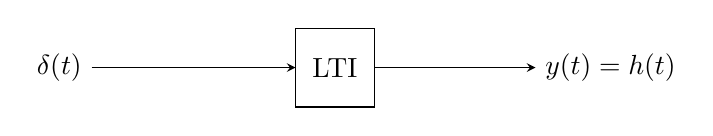
\begin{tikzpicture}
				\node (A) at (-3, 0) {\( \delta(t) \) };
				\node (B) at (4, 0) {\( y(t) = h(t)\) };
				\draw[-stealth] (A) -- (0, 0);
				\draw (0, -0.5) rectangle node {LTI } (1, 0.5);
				\draw[-stealth] (1, 0) -- (B);
			\end{tikzpicture}
		\end{center}
		If we send a signal \( \delta(t - \tau) \) into the system, then due to linear time invariance, the 
		system should output \( y(t - \tau) = h(t - \tau) \). 
	\item If we now send the signal \( x(\tau) \delta(t - \tau) \), then because \( x(\tau) \) is a constant, 
		then we invoke linearity to get that the output is  \( x(\tau) h(t - \tau) \). 
	\item Now, consider what happens when we send in the signal that is just a combination of all possible \( \tau \). 
		Each \( x(\tau) \) is a constant, so the output signal is of the form
		\[
		\int_{-\infty}^{\infty} x(\tau) \delta(t - \tau) \mapsto \int_{-\infty}^{\infty} x(\tau) h(t - \tau) 
		\diff \tau
		\] 
		But now notice that this signal can also be written as:
		\[
		\int_{-\infty}^{\infty} x(\tau) \delta(t - \tau) \diff \tau = x(t)
		\] 
		And so if we're sending in a signal \( x(t) \), then the output should be \( y(t) \)! Thus, we've proven that
		the impulse response is all we need in order to characterize \( y(t) \).
	\item For future reference, a convolution, denoted by \( x(t) * h(t) \), is defined as: 
		\[
		x(t) * h(t) = \int_{-\infty}^{\infty} x(\tau) h(t - \tau) \diff  \tau = \int_{-\infty}^{\infty} x(t - \tau)
		h(\tau) \diff \tau
		\] 
		this last equality shows that convolution is a commutative operation. 
\end{itemize}
\subsubsection{Impulse Response of 1st order LCCDE}
\begin{itemize}
	\item Recall the step response to LCCDE:
		\[
			\dv{y(t)}{t} + ay(t) = bx(t) = bu(t) \implies y_{\text{step}}(t) = 
			\left( \frac{b}{a}( 1 - e^{-at}) \right) u(t)
		\] 
	\item Given an impulse, which in this case can be written as: 
		\[
		\delta(t) = \lim_{\epsilon \to 0}\frac{u(t) - u(t - \epsilon)}{\epsilon}
		\] 
		This implies that the response \( h(t) \) is given by: 
		\[
		h(t) = \lim_{\epsilon \to 0 }\frac{y_{\text{step}}(t) - y_{\text{step}}(t - \epsilon)}{\epsilon} 
		= \lim_{\epsilon \to 0}
		\frac{\frac{b}{a}\left( e^{-a(t - \epsilon)}u(t - \epsilon) - e^{-at}u(t) \right) }{\epsilon}
		= be^{-at}u(t)
		\] 
		(verify this at home, the simplification makes use of the fact that \( e^{a\epsilon} \approx 
		1 + a\epsilon + a^2 \frac{\epsilon^2}{2} + \cdots\), but the higher order terms die).
\end{itemize}
\subsection{Harmonic Response of an LTI system}
\begin{itemize}
	\item The response of an LTI system to a complex signal \( x(t) = Ae^{j \omega t} \) is always going to be another 
		complex exponential signal \( y(t) = H(\omega) Ae^{j \omega t} \)
	\item Given the input signal \( x(t) = Ae^{j \omega t} \), we can write:
		\begin{align*}
			y(t) &= \int_{-\infty}^{\infty} x(\tau) h(t - \tau) \diff \tau\\
				 &= \int_{-\infty}^{\infty} Ae^{j \omega t}
			h(t - \tau) \diff \tau \\
				 &= \int_{-\infty}^{\infty} Ae^{j \omega (t - \tau')}h(\tau') \diff \tau'\\
				 &= Ae^{j \omega t}\underbrace{\int_{-\infty}^{\infty} e^{-j \omega \tau'}h(\tau') \diff \tau'}_{
				 H(\omega)}\\
				 &= H(\omega) Ae^{j \omega t} 
		\end{align*} 
	\item By definition:
		\[
		H(\omega) \equiv \int_{-\infty}^{\infty} e^{-j \omega \tau'}h(\tau') \diff \tau' \ \ 
		H(f) \equiv \int_{-\infty}^{\infty} e^{-j 2 \pi ft}h(t) \diff t 
		\] 
		You'll recognize \( H(\omega) \): it's the Fourier transform equation.
		
		\question{When given an harmonic input, and we're asked to measure it, are we measuring the real part 
		of the signal?}
\end{itemize}
\subsubsection{Example: Frequency response of an RC Circuit}
\begin{itemize}
	\item Given the following circuit:
		% insert circuitkkz
	\item The impulse response is given by the differential equation:
		\[
			\dv{y(t)}{t} + \frac{1}{RC}y(t) = \frac{1}{RC}x(t)
		\] 
		This is a first order LCCDE, so therefore the impulse response \( h(t) \) is given by 
		\( h(t) = be^{-at}u(t) \). 
	\item For the frequency response, we have a function of the form \( x(t) = e^{j \omega t} \), 
		which we know has an output signal of the form \( y(t) = H(\omega) e^{j \omega t} \). So all that remains
		now is to find \( H(\omega) \) :
		\begin{align*}
			y(t) &= e^{j \omega t }\int_{-\infty}^{\infty} e^{-j \omega t}h(\tau) \diff  \tau \\
			&= e^{j \omega t}\int_{-\infty}^{\infty} be^{-a\tau}u(\tau) e^{-j \omega \tau}\diff \tau  \\
			&= be^{j \omega t}\int_{0}^{\infty} e^{-a \tau}e^{-j \omega \tau}\diff \tau  \\
			&= \left( \left.-\frac{1}{a + j \omega}e^{-a \tau}e^{-j \omega t}\right|_0^{\infty}\right)
				be^{j \omega t} \\
				&= \frac{b}{a + j \omega}e^{j \omega t} 
		\end{align*}
		Now, if we impose that \( a = b = \frac{1}{RC} \), then we get the equation: 
		\[
		\frac{\frac{1}{j c \omega}}{\frac{1}{j c \omega} + R}e^{ j \omega t}
		\] 
		Now, \( \frac{1}{jc\omega} \) is the impedance of a capacitor, and this overall equation takes the form of a 
		voltage divider for a circuit with known impedance: 
		\[
		y(t) = \frac{z(\omega)}{z(\omega) + R}e^{j \omega t}
		\] 
\end{itemize}
\subsection{Sinusoidal Input} 
\begin{itemize}
	\item With the harmonic response tools, we can now evaluate the system response when given a sinusoidal 
		input, since we know that 
		\[
		\cos(\omega t) = \frac{e^{ j \omega t} + e^{- j \omega t}}{2}
		\] 
		\question{Does the same work with sine, where there's a complex number is in the denominator?} 
\end{itemize}
\subsection{LTI systems in Parallel and Series}
\begin{itemize}
	\item For a basic system with a single input and output, 
		we've already discussed that \( y(t) = x(t) * h(t) \). Now, what if we connect these systems in 
		parallel?
		\begin{center}
			\begin{tikzpicture}
				\node (A) at (-3, 0) {\( x(t) \) };
				\node (B) at (4, 0) {\( y(t) \) };
				\node (C) at (1.5, 0) {+};
				\draw[-stealth] (A) -- (-0.5, 0) -- (-0.5, 1) -- (0, 1);
				\draw (0, 0.5) rectangle node {\( h_1(t) \) } (1, 1.5);
				\draw[-stealth] (-0.5, 0) -- (-0.5, -1) -- (0, -1);
				\draw (0, -0.5) rectangle node {\( h_2(t) \) } (1, -1.5);
				\draw[-stealth] (1, 1) -- (1.5, 1) -- (C);
				\draw (C) circle (0.2cm);
				\draw[-stealth] (C) -- (B);
				\draw[-stealth] (1, -1) -- (1.5, -1) -- (C);
			\end{tikzpicture}
		\end{center}
		then, the result \( y(t) \) is given by \( y(t) = x(t) * h_1(t) + x(t) * h_2(t) = x(t) * 
		(h_1(t) + h_2(t))\).
	\item If we connect them in series: 
		\begin{center}
			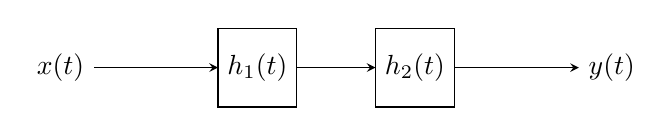
\begin{tikzpicture}
				\node (A) at (-3, 0) {\( x(t) \) };
				\node (B) at (4, 0) {\( y(t) \) };
				\draw[-stealth] (A) -- (-1, 0);
				\draw (-1, -0.5) rectangle node {\( h_1(t) \) } (0, 0.5);
				\draw[-stealth] (0, 0) -- (1, 0);
				\draw (1, -0.5) rectangle node { \( h_2(t) \) } (2, 0.5);
				\draw[-stealth] (2, 0) -- (B);
			\end{tikzpicture}
		\end{center}
		then	
\end{itemize}

	\section{Polynomial Multiplication II}
\begin{itemize}
	\item As a recap, we have two polynomials \( p \) and \( q \), both of degree \(  n -1 \), and we want to multiply 
		them. 
	\item We saw the \textit{coefficient representation}, where we specify its coefficients. So for \( p \), we have \( (p_0, p_1, 
		\dots, p_{n-1})\). Last lecture, we saw \( O(n^2) \) algorithm to multiply the polynomials using the 
		coefficient representation.
	\item We also saw the \textit{value representation}, where instead of giving the polynomial itself we give a set of 
		\( m \) points that the polynomial passes through. As long as \( m \ge  n \), then this set of points 
		fully specifies the polynomial. With this representation, we saw that polynomials can be multiplied in \( O(n) \) time. 
	\item So our main question was: is there a way for us to use the value representation to speed up the coefficient 
		representation multiplication?
	\item Roots of unity: the set of points we will evaluate our polynomials on. 
\end{itemize}
\subsection{Fast Fourier Transform}
\begin{itemize}
	\item Input: \( m \), a power of 2, a \( p(x) = p_0 + p_1x + \cdots + p_{m-1}x^{m-1} \). Our goal is to evaluate 
		 \( p( \omega_0), p(\omega_1), \dots, p(\omega_{m - 1}) \). 
	 \item We will use a divide and conquer approach:
		 \begin{center}
		 	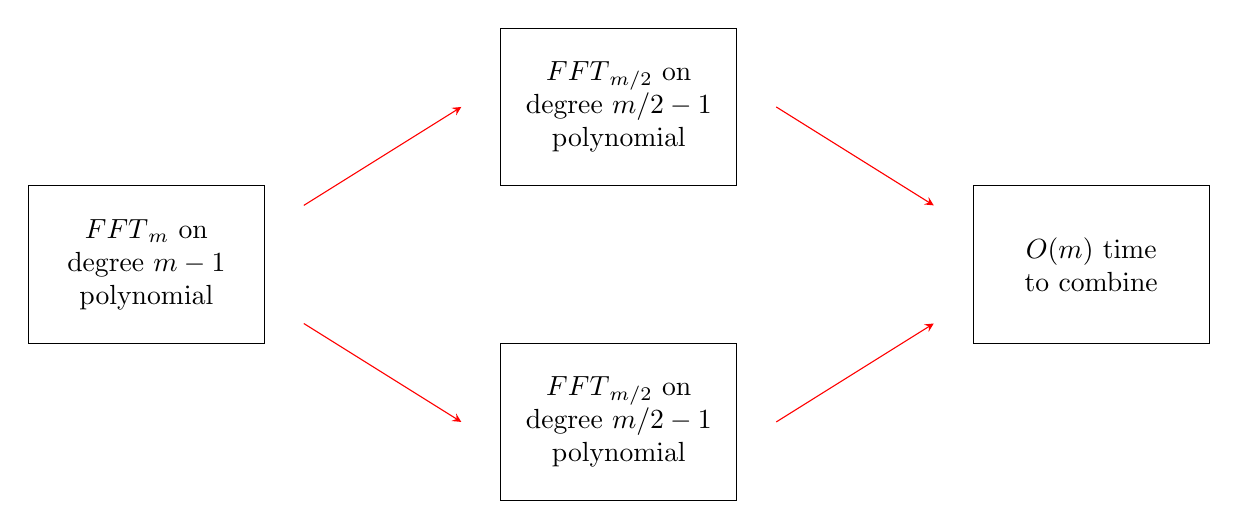
\begin{tikzpicture}[every text node part/.style={align=center}]
		 		\draw(0, -1) -- (3, -1) -- (3, 1) -- (0, 1) -- cycle;
				\draw(6, 1) -- (9, 1) -- (9, 3) -- (6, 3) -- cycle;
				\draw(6, -1) -- (9, -1) -- (9, -3) -- (6, -3) -- cycle;
				\draw(12, -1) -- (15, -1) -- (15, 1) -- (12, 1) -- cycle;
				\draw node at (1.5, 0) {\( \text{FFT}_m \) on \\degree \( m - 1 \) \\ polynomial}; 
				\draw node at (7.5, 2) { \( \text{FFT}_{m / 2} \) on \\ degree \( m / 2 - 1 \) \\ polynomial};
				\draw node at (7.5, -2) { \( \text{FFT}_{m / 2} \) on \\ degree \( m / 2 - 1 \) \\ polynomial};
				\draw node at (13.5, 0) {\( O(m) \) time \\ to combine};
				\draw[-stealth, red] (3.5, 0.75) -- (5.5, 2);
				\draw[-stealth, red] (3.5, -0.75) -- (5.5, -2);
				\draw[-stealth, red] (9.5, 2) -- (11.5, 0.75);
				\draw[-stealth, red] (9.5, -2) -- (11.5, -0.75); 
		 	\end{tikzpicture}
		 \end{center}
		 This will give us a recurrence relation \( T(m) \le  2 \cdot T(m / 2) + O(m) \), and from the master theorem this 
		 gives an \( O(m \log m) \) runtime.
\end{itemize}
\subsection{Divide and Conquer}
\begin{itemize}
	\item To figure out how to divide, let's first write out \( p(x) \) :
		\[
		p(x) = p_0 + p_1x + p_2x^2 + p_3x^3 + \cdots
		\] 
		Let's split \( p \) into two parts, based on the parity of the exponent. We'll call these the even and odd 
		halves:
		\begin{align*}
			p_E(x) &= p_0 + p_2x^2 + p_4x^{4} + \cdots + p_{m - 2}x^{m - 2}\\
			p_O(x) &= p_1x + p_3x^3 + \cdots + p_{m - 1} x^{m - 1} 
		\end{align*}
		But notice that we can rewrite the even part a little bit:
		\[
		p_E(x) = p_0 + p_2(x^2) + p_4(x^2)^2 + p_6(x^2)^3 + \cdots = \text{Even}(x^2)
		\] 
		But this looks like a polynomial with coefficietns \( p_0, p_2, p_4, \dots \) evaluated on \( x^2 \)! We will call 
		this polynomial \( \text{Even}(z) \). For the odd part, we factor out an \( x \) :
		\[
		p_1x + p_3x^3 + \cdots = x(p_1 + p_3x^2 + p_5x^{4} + \cdots) = x \cdot \text{Odd}(x^2)
		\] 
		The key to note here is that we have a recursion in the fact that we can express the evaluation of the polynomials 
		at the \( n \)-th step as a computation involving another polynomial but evaluated on \( x^2 \). So, we have 
		\[
		p(x) = \text{Even}(x^2) + x \cdot \text{Odd}(x^2)
		\] 
		The degree of the even part is \( (m - 2) / 2 = m / 2 - 1 \), and the same goes for odd part.   
	\item Now if we want to compute \( p \) on \( \omega_i \), then we have \( p(\omega_i) = \text{Even}(\omega_i^2) + 
		\omega_i \cdot \text{Odd}(\omega_i^2)\). 
	\item Because we are squaring the arguments, then this means that we are evaluating the Even and Odd parts on the 
		\( m / 2 \)-th roots of unity, because of our magical fact!
	\item So to compute \( p(\omega_i) \), we recursively evaluate the even and odd parts at the  \( m / 2 \)-th roots of unity:
		\( \alpha_0, \alpha_1, \dots, \alpha_{m / 2 - 1} \). 
	\item To combine, all we need to do is multiply the odd part by  \( \omega_i \), then add the two parts together. So, the 
		combination step only takes \( O(m) \) work. So this fully gives our recursion \( T(m) \le  2 \cdot T(m / 2) + O(m) \), 
		hence the \( O(m \log m) \) runtime. 
\end{itemize}
\subsection{Fast Interpolation}
\begin{itemize}
	\item An update on our algorithm scheme:
		\begin{center}
			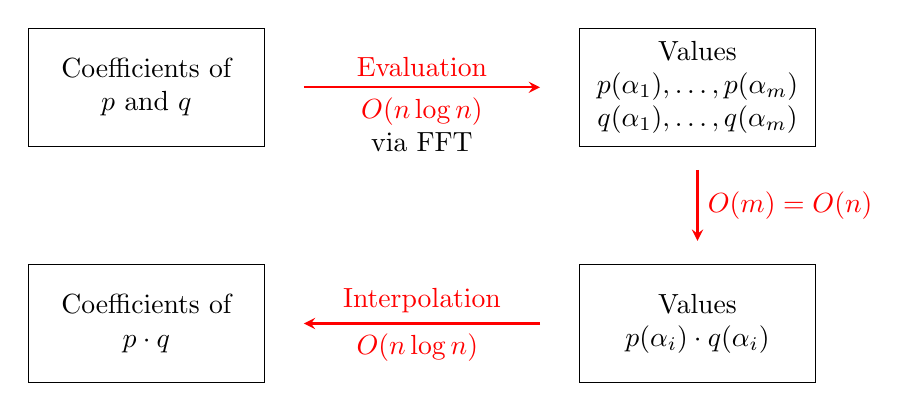
\begin{tikzpicture}[every text node part/.style={align=center}]
				\foreach \x in {0, 7}
				\foreach \y in {0, 3}
				{
					\draw (\x, \y) -- (\x+3, \y) -- (\x+3, \y+1.5) -- (\x, \y+1.5) -- cycle;
				}
				\draw node at (1.5, 0.75) {Coefficients of \\ \( p \cdot q \)};
				\draw node at (1.5, 3.75) {Coefficients of \\ \( p \) and \( q \) };
				\draw node at (8.5, 0.75) {Values \\ \( p(\alpha_i) \cdot q(\alpha_i) \) };
				\draw node at (8.5, 3.75) {Values \\ \( p(\alpha_1), \dots, p(\alpha_m) \) \\ \( q(\alpha_1), \dots, q(\alpha_m) \) };
				\draw[-stealth, red, thick] (3.5, 3.75) --node[midway, above] {Evaluation} node[midway, below] 
					{\( O(n \log n) \) \\ \textcolor{black}{via FFT}} (6.5, 3.75); 
				\draw[-stealth, red, thick] (8.5, 2.7) -- node[midway, right] {\( O(m) = O(n) \) } (8.5, 1.8);
				\draw[-stealth, red, thick] (6.5, 0.75) -- node[midway, above] {Interpolation} node[midway, below] 
					{\( O(n \log n) \) } (3.5, 0.75);
			\end{tikzpicture}
		\end{center}
	\item Now we want to figure out the interpolation step: given \( r(\omega_0), r(\omega_1), \dots, r(\omega_{m - 1}) \), we want 
		to get back the coefficient representation of \( r(x) \). This is called the inverse FFT. 
	\item It turns out that when we do the Fourier transform, we basically get the inverse Fourier transform for free. Recall 
		the Fourier transform:
		\[
			p(\omega_\ell) = \sum_{j = 0}^{m - 1}p_j (\omega_\ell)^{j}
		\]
		This equation comes from replacing all \( x \) 's with \( \omega_\ell \). Then, the inverse Fourier transform is written 
		as follows:
		\[
			p_{\ell} = \frac{1}{m} \cdot \sum_{j = 0}^{m - 1}p(\omega_j) \cdot (\omega_{m - \ell})^{j} = \frac{1}{m} \cdot 
			q(\omega_{m - \ell})
		\] 
		Here, \( q(x) = p(\omega_0) + p(\omega_1)x + \cdots p(\omega_{m - 1})x^{m - 1} \). So in essence, this is basically another 
		polynomial evaluation, which we already know happens in \( O(m \log m) = O(n \log n) \) time!
	\item So, now let's look at the completed diagram:
		\begin{center}
			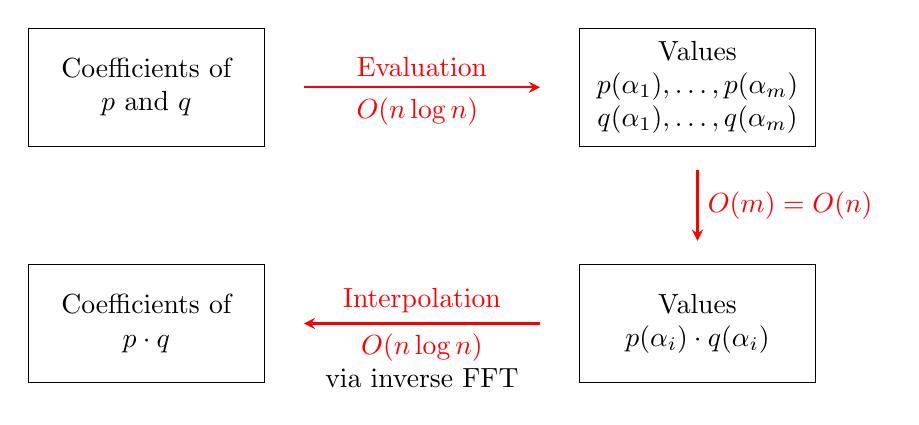
\begin{tikzpicture}[every text node part/.style={align=center}]
				\foreach \x in {0, 7}
				\foreach \y in {0, 3}
				{
					\draw (\x, \y) -- (\x+3, \y) -- (\x+3, \y+1.5) -- (\x, \y+1.5) -- cycle;
				}
				\draw node at (1.5, 0.75) {Coefficients of \\ \( p \cdot q \)};
				\draw node at (1.5, 3.75) {Coefficients of \\ \( p \) and \( q \) };
				\draw node at (8.5, 0.75) {Values \\ \( p(\alpha_i) \cdot q(\alpha_i) \) };
				\draw node at (8.5, 3.75) {Values \\ \( p(\alpha_1), \dots, p(\alpha_m) \) \\ \( q(\alpha_1), \dots, q(\alpha_m) \) };
				\draw[-stealth, red, thick] (3.5, 3.75) --node[midway, above] {Evaluation} node[midway, below] 
					{\( O(n \log n) \) } (6.5, 3.75); 
				\draw[-stealth, red, thick] (8.5, 2.7) -- node[midway, right] {\( O(m) = O(n) \) } (8.5, 1.8);
				\draw[-stealth, red, thick] (6.5, 0.75) -- node[midway, above] {Interpolation} node[midway, below] 
					{\( O(n \log n) \) \\ \textcolor{black}{via inverse FFT}} (3.5, 0.75);
			\end{tikzpicture}
		\end{center}
		So this shows that polynomial multiplication can be done in \( O(n \log n) \) time!  
\end{itemize}
\subsection{The Matrix Viewpoint}
\begin{itemize}
	\item There's another way to represent \( p(x) \), as a column vector:
		\[
		\begin{bmatrix} p(\omega_0)\\p(\omega_1)\\p(\omega_2)\\ \vdots \\ p(\omega_{m - 1}) \end{bmatrix} = 
		\begin{bmatrix} p_0 + p_1\omega_0 + p_2 \omega_0^2 + \cdots + p_{m-1}\omega_0^{m- 1}\\
		p_0 + p_1 \omega_1 + p_2\omega_1^2 + \cdots + p_{m-1}\omega_1^{m-1}\\
	\vdots \\
p_0 + p_1\omega_{m-1} + p_2\omega_{m-1}^2 + \cdots+ p_{m-1}\omega_{m-1}^{m-1}\end{bmatrix} 
= \underbrace{\begin{bmatrix} 1 & \omega_0 & \omega_0^2 & \dots & \omega_0^{m-1}\\
1 & \omega_1 & \omega_1^2 & \dots & \omega_1^{m-1}\\
1 & \omega_2 & \omega_2^2 & \dots & \omega_2^{m-1}\\
\vdots & \vdots & \vdots & \ddots & \vdots\\
1 & \omega_{m-1} & \omega_{m-1}^2 & \dots & \omega_{m-1}^{m-1}\end{bmatrix}}_{M} \cdot \underbrace{\begin{bmatrix} p_0\\p_1\\p_2\\ \vdots \\p_{m-1} \end{bmatrix}}_{[p]} 
		\] 
	\item If we didn't know FFT, then this computation is just a matrix multiplied by a vector, whihc would take \( O(m^2) \)  
		time. However, FFT basically gives us a way to compute this matrix in \( O(m \log m) \) time!

		Note also that this also solves this \textbf{without ever writing down \( M \) !} 
	\item The Inverse FFT looks much cleaner in this representation:
		\[
		M^{-1} \cdot \begin{bmatrix} p(\omega_0)\\p(\omega_1)\\p(\omega_2)\\ \vdots \\ p(\omega_{m-1}) \end{bmatrix} = 
		\begin{bmatrix} p_0\\p_1\\p_2\\ \vdots \\ p_{m-1} \end{bmatrix} 
		\] 
	\item For \( M \) specifically, we have \( M_{ij} = \omega_i^{j} = (\omega_1^{i})^{j} = \omega_1^{ij} \). Then, the inverse 
		is defined as: \( (M^{-1})_{ij} = \frac{1}{n} \cdot \omega_{m-i}^{j} \). 
\end{itemize}
\subsection{Applications}
\begin{itemize}
	\item \textbf{Cross Correlation:}
		Given the product of \( p(x) = p_0 + p_1x + p_2x^2 + p_3x^3 \) and \( q(x) = q_0 + q_1x + q_2x^2 + q_3x^3 \), the 
		coefficient on \( x^{i} \) in \( p(x) \cdot q(x) \) is
		\[
		p_0q_{i} + p_1q_{i-1} + \cdots + p_{i-1}q_{1} + p_{i}q_0
		\] 
		Now consider two arrays \( [p_0, p_1, p_2, p_3] \) and \( [q_3, q_2, q_1, q_0] \). Now let's stack them on top of each 
		other and take the dot product of the overlap. Depending on where they overlap, it actually corresponds to the coefficient 
		on some \( x^{i} \) in \( p(x) \cdot q(x) \).  
		\begin{center}
			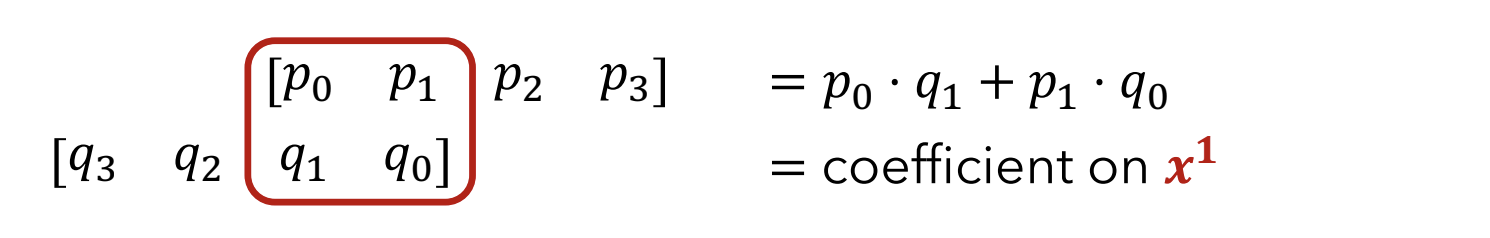
\includegraphics[scale=0.5]{cross-correlation.png}
		\end{center}
		This is called \textbf{cross-correlation}, and due to FFT, we can compute these in \( O(n \log n) \) time.   
	\item  \textbf{Integer Multiplication:} Say we wanted to multiply \( a = a_{n-1} \cdots a_2a_1a_0 \) and 
		\( b = b_{n-1}\cdots b_2b_1b_0 \). We can write down these two polynomials:
		\begin{align*}
			A &= a_0 + a_1x + a_2x^2 + \cdots + a_{n-1}x^{n-1}\\
			B&= b_0 + b_1x + b_2x^2 + \cdots + b_{n-1}x^{n-1} 
		\end{align*}
		and to compute the product, we can write \( A(x) \cdot B(x) \) and plug in \( x = 10 \). Naively we would think that 
		this takes \( O(n \log n) \) time, but this is not exactly true. This is because here, our additions and multiplications 
		don't exactly happen in \( O(1) \) time anymore, so we have to be careful! In fact, the multiplication can be as 
		large as \( \Theta(n) \). 

		After keeping track of all this, we get an \( O(n \log n \log \log n) \) algorithm. 
	\item \textbf{Fourier Transform:} FFT allows us to compute the Fourier transform of \( p(x) \) quickly -- we can decompose 
		 \( p(x) \) into its consistuent sines and cosines. There are too many applications of the Fourier transform to 
		 even list: 
		 \begin{enumerate}[label=\arabic*.]
		 	\item Music software
			\item Heart rate monitor
			\item Signal processing (e.g. cell phones)
			\item Many more!
		 \end{enumerate}
		 The fact that quantum computers can compute Fourier transforms exceedingly quickly is actually one of the main reasons 
		 that makes them so powerful.
\end{itemize}

	\section{Lecture 6}
\subsection{Clarification on BIBO Stability}
\begin{itemize}
	\item When we say a "bounded" signal, we mean that the amplitude of the signal is bounded at all times:
		\[
		|x(t)| < \infty \ \forall t \in \R
		\] 
		The same definition follows for discrete-time signals. 
	\item For LTI systems, we call the system BIBO stable if and only if its impulse \( h(t) \) is absolutely 
		integrable:
		\[
		\int_{-\infty}^{\infty} |h(t)| \diff t < \infty
		\] 
\end{itemize}
\subsection{Cross-Correlation}
\begin{itemize}
	\item The cross correlation between two signals \( r_{xy}(t) = r_{yx}(-t) \). To show this explicitly, we 
		look at the cross-correlation equation:
		\begin{align*}
			r_{xy}(t) &= \int_{-\infty}^{\infty} x(\tau)y(t + \tau) \diff \tau \\
			r_{yx}(t) &= \int_{-\infty}^{\infty} y(\tau) x(t + \tau) \diff \tau  
	\end{align*} 
	But for the second equation, we can define a \( \tau' = t + \tau\), so then we get: 
	\[
	r_{yx}(t) = \int_{-\infty}^{\infty} y(\tau' - t)x(\tau') \diff \tau' = \int_{-\infty}^{\infty} 
	x(\tau') y(-t + \tau') \diff \tau'
	\] 
	This looks like the first equation except we have \( -t \) instead of \( t \). Therefore, we have 
	\( r_{xy}(t) = r_{yx}(-t) \). The same works for discrete time: \( r_{xy}[n] = r_{yx}[-n] \). 
\end{itemize}

\subsection{More Convolution Properties} 
\begin{itemize}
	\item \textbf{Differentiation property:} Given \( y(t) = x(t) * h(t) \), then:
		\[
			\dv{t} y(t) = x(t) * \dv{h(t)}{t} = \dv{x(t)}{t} * h(t)
		\] 
	\item \textbf{Intergration Property:} Given \( y(t) = x(t) * h(t) \), we have:
		\[
		\int_{-\infty}^{t'} y(t) \diff  t = x(t) * \int_{-\infty}^{t'} h(\tau)\diff \tau 
		\] 
\end{itemize}
\subsection{Fourier Transform} 
\begin{itemize}
	\item The fourier transform came from the study of the heat equation, written as:
		\[
			c \rho \pdv{t} u(x, y, z, t) = k \left( \pdv[2]{x} + \pdv[2]{y} + \pdv[2]{z} \right) 
			u(x, y, z, t)
		\] 
		Fourier then claimed that the solution can be expanded in a series of sines with multiples of the variable. 
		In other word,s the solution is of the form:
		\[
		f(x) = \frac{1}{2a_0} + (a_1 \sin(x) + b_2 \cos(x)) + (a_2\sin(2x) + b_2\cos(2x)) + \cdots 
		\] 
	\item Recall the frequency response of an LTI system:
		\begin{center}
			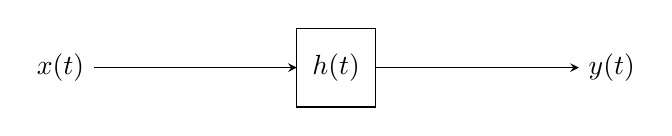
\begin{tikzpicture}
				\node (A) at (-3, 0) {\( x(t) \) };
				\node (B) at (4, 0) {\( y(t) \) };
				\draw[-stealth] (A) -- (0, 0);
				\draw (0, -0.5) rectangle node {\( h(t) \) } (1, 0.5);
				\draw[-stealth] (1, 0) -- (B);
			\end{tikzpicture}
		\end{center}
		Recall that we can characterize \( y(t) \) via a convolution: 
		\[
		y(t) = \int_{-\infty}^{\infty} x(\tau) h(t - \tau) \diff  \tau 
		\] 
		If we do this with our input \( e^{j 2 \pi ft} \), then we get:
		\[
		y(t) = H(f) e^{j 2 \pi ft} = H(\omega) e^{j \omega t }
		\] 
		Here, \( H(\omega) \) is defined to be the Fourier transfrm of the impusle response \( h(t) \):
		\[
			H(\omega) = \int_{-\infty}^{\infty} e^{- j \omega t} h(t) \diff t 
		\] 
		Alternatively, written in frequency language:
		\[
		H(f) = \int_{-\infty}^{\infty} e^{-j 2 \pi ft}h(t) \diff t 
		\] 
	\item Formally, the Fourier transform is defined as:
		\[
		H(f) \equiv \mathcal F \{h(t)\} \equiv \int_{-\infty}^{\infty} h(t) e^{-j 2\pi ft }\diff  t 
		\] 
		This transforms the signal \( h(t)  \) from the time domain into the frequency domain. The reason for this 
		is becuase the Fourier transform is a definite integral, which kills off any \( t \) dependence entirely. 
		In terms of angular frequency, we have:
		\[
		H(\omega) \equiv \mathcal F \{h(t)\} = \int_{-\infty}^{\infty} h(t) e^{-j \omega t}\diff t 
		\] 
	\item The inverse Fourier transform is:
		\[
			h(t) = \mathcal F^{-1} \{H(f)\} = \int_{-\infty}^{\infty} H(f) e^{j 2\pi ft}\diff  f 
		\]
		Since the Fourier transform takes objects from the time domain to the frequency domain, the inverse 
		Fourier transform takes things from the frequency domain to the time domain. 

		In terms of angular frequency, we have:
		\[
		h(t) = \mathcal F^{-1} \{H(\omega)\} = \frac{1}{2\pi}\int_{-\infty}^{\infty} H(\omega) 
		e^{j \omega t}\diff \omega 
		\] 
		This is also sometimes called the "synthesis equation", since we basically create \(  x(t) \) out of 
		\( H(\omega) \). 
	\item We can also provably show that the Inverse fourier transform does indeed invert the Fourier transform, 
		albeit with a lot of algebra. See lecture slides for the full derivation.  
	\end{itemize}

	\section{Lecture 7}
\subsection{DTFT and Convergence}
\begin{itemize}
	\item Not all functions have a Fourier transform, and the problem of whether a function has a Fourier 
		integral is an incredibly complex problem with no simple statement. 
	\item However, we know that there are several sufficient (but not necessary) conditions. Firstly, 
		we know that \( x(t) \) must be absolutely integrable. That is, 
		\[
		\int_{-\infty}^{\infty} |x(t)| \diff t < \infty
		\] 
\end{itemize}
\subsection{Fourier Transform Pairs}
\begin{itemize}
	\item There are several pairs of Fourier transforms that are useful to memorize.
	\item The Delta function:
		\[
			x(t) = \delta(t - t_0) \leftrightarrow X(f) = e^{-j 2\pi ft_0}
		\]
		This actually has strong implications about the nature of the Fourier transform -- there is an 
		"uncertainty principle" that manifests itself here. A signal cannot be both localized in time and frequency at
		the same time.
	\item Complex exponentials:
		\[
		x(t) = e^{j \omega_0 t} = e^{j 2 \pi f_0 t} \leftrightarrow X(f) = \delta(f - f_0)
		\] 
		This is the same as the previous point, except now we're going backwards.   
	\item Cosine functions:
		\[
		x(t) = \cos(2 \pi f_0 t) \leftrightarrow X(f) = \frac{1}{2}\delta(f - f_0) + \delta(f + f_0))
		\] 
		This makes sense: a plane wave is a composition of a left and right travelling wave.  
	\item Sine functions:
		\[
		x(t) = \sin(2 \pi f_0 t) \leftrightarrow X(f) = \frac{1}{2j}(\delta(f - f_0) - \delta(f + f_0))
		\] 
		Note that the only difference here is the minus sign, as a result of the conversion of sine into 
		complex exponentials.
	\item Shah function:
		\[
		x(t) = III(t) \leftrightarrow X(f) = III(f) \text{ or } X(\omega) = \frac{1}{2\pi}III(\omega)
		\] 
	\item Rect function:
		\[
		x(t) = \sqcap(t) \leftrightarrow \sinc(f)
		\] 
\end{itemize}

	\section{Fourier Transforms}
\subsection{Discrete Fourier Transform}
\begin{itemize}
	\item Recall the Shah function: \( x(t) = \text{III}(t) = \sum_{k = -\infty}^{\infty}\delta(t - k) \). Its 
		fourier transform in ordinary frequency is: 
		\[
		X(f) = \int_{-\infty}^{\infty} \sum_{k = -\infty}^{\infty} \delta(t - k) e^{-j 2 \pi f t}\diff t
		= \sum_{n = -\infty}^{\infty} \delta(f - n) = III(f)
		\] 
		So the Fourier transform of a Shah function is itself a shah function, in frequency space.  
	\item In Angular frequency (\( \omega \) ), then it's writtne as: 
		\[
		X(\omega) = X(f) = 2\pi \sum_{n = -\infty}^{\infty} \delta(2 \pi f - 2\pi n) = 2\pi \sum_{n = -\infty}^{\infty}
		\delta(\omega - 2 \pi n)
		\] 
\end{itemize}
\subsection{Convolutions and Fourier Transform} 
\begin{itemize}
	\item There is an identity between the Fourier transform and convolution, called the convolution theorem: 
		\[
		x_1(t) * x_2(t) \leftrightarrow X_1(f) X_2(f)
		\] 
		The right hand side can also be replaced by \( X_1(\omega) X_2(\omega) \), up to a normalization factor. 
		This equation basically says that the Fourier transform of the convolution of two function is also equal to the
		pointwise product of the Fourier transforms of \( x_1 \) and \( x_2 \). 

		\begin{proof}
			Start with the Fourier transform of \( x_1(t) * x_2(t) \) :
			\[
			\int_{-\infty}^{\infty} (x_1(t) * x_2(t)) e^{-j 2 \pi ft}\diff t = \int_{-\infty}^{\infty} \left( 
			\int_{-\infty}^{\infty} x_1(\tau) x_2(t - \tau) \diff \tau \right) e^{-j 2 \pi ft}\diff t 
			\] 
			Now, we take the \( t \) integral first becuase it's easier: 
			\[
			\int_{-\infty}^{\infty} x_1(\tau) \int_{-\infty}^{\infty} x_2(t - \tau) e^{-j 2 \pi ft}\diff t  \diff \tau
			= \int_{-\infty}^{\infty} x_1(\tau) e^{-j 2 \pi f\tau}X_2(f) \diff \tau = X_1(f) X_2(f) 
			\] 
		\end{proof}
	\item For example, consider the rect function \( \sqcap(t) \) that is 1 on the interval \( [-1 / 2, 1/2] \). 
		If we do the Fourier transform of this, we get a sinc function. At \( f = 0 \), we have 
		\( \sinc(f) = 1 \). 

		If we wanted to take the FT of the convolution of two rect functions, then we can use the convolution theorem 
		to conclude that \( \mathcal F(\sqcap(t)) = \sinc^2(f) \). Conversely, we know that the inverse Fourier 
		transform of \( \sinc^2(f) \) would be the triangular function, becuase we know that it's the convolution 
		of two rect functions.
\end{itemize}
\subsection{Fourier Series}
\begin{itemize}
	\item Consider a periodic function, where \( x(t) = x(t + nT) \). One way to write \( x(t) \) and also to 
		reflect its period, we can write it as a sum of delta functions: 
		\[
		x(t) = \sum_{n=-\infty}^{\infty} \left( x(t) \sqcap\left( \frac{t}{T} \right)  \right) * \delta(t - nT) 
		\] 
		Basically the rect function restricts the domain to only one period of \( x(t) \), and we convolve this with 
		a series of Delta functions in order to generate the roiginal fnction back. We can also do some simplifications
		on this: 
		\[
		x(t) = \left( x(t) \sqcap\left( \frac{t}{T} \right)  \right) * \sum_{n=-\infty}^{\infty} \delta(t - nT) 
		\] 
		Then we can use an identity to get: 
		\[
		x(t) = \left( x(t) \sqcap\left( \frac{t}{T} \right)  \right) \frac{1}{T}\text{III}\left( \frac{t}{T} \right) 
		\] 
		\question{How did we get the simplification of the delta sum into the Shah function?} 
	\item Turns out, if we perform a Fourier transform of \( x(t) \), then we get a discrete set of values, 
		also called a Fourier series. Taking the Fourier transform of the above function, and defining 
		\( g(t) = x(t) \sqcap(t / T) \), then we can write: 
		\begin{align*}
			\mathcal F \{x(t)\} &= \mathcal F \left\{g(t) * \frac{1}{T}\text{III}\left( \frac{t}{T} \right) \right\}  \\
								&= \mathbf G(f) \text{\textbf{III}} (Tf)
		\end{align*}
		where \( \mathbf G(f) \) is the Fourier transform of \( g(t) \).  Expanding the Shah function out, we 
		have: 
		\[
		\frac{1}{T}\sum_{n=-\infty}^{\infty} \mathbf G(f) \delta\left( f - \frac{n}{T} \right) 
		\] 
		The delta function will select \( f = \frac{n}{T} = nf_0\), so we get: 
		\[
		\frac{1}{T}\sum_{n=-\infty}^{\infty} G(nf_0) \delta\left(f - \frac{n}{T}\right)
		\] 
	\item So, from here we can conclude that the Fourier transform of a periodic function is just a series over that 
		function. 
	\item The inverse Fourier transform used to be:
		\[
		x(t) = \int_{-\infty}^{\infty} \mathbf X(f) e^{j 2 \pi ft}\diff f 
		\] 
		Where \( \mathbf X(f) \) is the (continuous-time) Fourier transform of \( x(t) \). Since \( x \) is periodic, 
		then we can write
		\begin{align*}
			x(T) &= \int_{-\infty}^{\infty} \sum_{n=-\infty}^{\infty} \mathbf G(n) \delta\left( f - \frac{n}{T} \right) 
		e^{j 2 \pi ft }\diff  f\\
		&= \frac{1}{T}\sum_{n=-\infty}^{\infty} \mathbf G(n) \int_{-\infty}^{\infty} \delta\left( f - \frac{n}{T} \right) e^{j 2 \pi ft} \diff  f  \\
		&= \frac{1}{T}\sum_{n=-\infty}^{\infty} \mathbf G(n) e^{2 \pi \frac{n}{T}t}\\
		&= \frac{1}{T}\sum_{n=-\infty}^{\infty} \mathbf G(n) e^{j 2 \pi n f_0 t} 
		\end{align*} 
		Note that the delta function only picks out the frequency \( \frac{n}{T} \), which allows us to get a discrete
		sum of frequencies. This is called the Discrete Fourier Series. 
\end{itemize}

	\section{More on Fourier Transforms}
\subsection{Discrete Time Fourier Transforms (DTFT)}
\begin{itemize}
	\item Recall that for continuous time signals, the fourier transform is written as 
		\[
		X(\omega) = \int_{-\infty}^{\infty} x(t) e^{-j \omega t}\diff t 
		\] 
	\item For discrete time signals, the way to do this is to write the signal as a continuous time signal 
		via delta functions, and then apply CTFT:
		 \[
			 x(t) = \sum_{n=-\infty}^{\infty} x[n] \delta(t - n)
		\] 
		Then, we can write:
		\[
			X(\omega) = \sum_{n=-\infty}^{\infty} x[n] \int_{-\infty}^{\infty} \delta(t - n) e^{-j \omega t}\diff t
			= \sum_{n=-\infty}^{\infty} x[n] e^{- j \omega n }
		\] 
		So this actually just means that in discrete time, the Fourier transform of \( x[n] \) is just 
		the amplitude of the signal at that particular \( n \), multiplied by a sinusoid of a corresponding 
		frequency specified by \( n \). 
	\item In general, we have:
		\begin{align*}
			X(e^{j 2 \pi f}) &= \sum_{n=-\infty}^{\infty} x[n] e^{-j 2 \pi f n} & x[n] &=
			\int_{-\infty}^{\infty} X(e^{j 2 \pi f})e^{j 2 \pi f n}\diff f \\
			X(e^{j \omega}) &= \sum_{n=-\infty}^{\infty} x[n] e^{-j \omega n} & x[n] &= \frac{1}{2\pi}
			\int_{-\infty}^{\infty} X(e^{j \omega}) e^{j \omega n}\diff  \omega 
		\end{align*}
		Sometimes textbooks use \( \Omega \) insetad of \( \omega \), but we will use the latter.   
	\item See lectures for worked examples on how to do this.
\end{itemize}

\subsection{Characteristics of DTFT}
\begin{itemize}
	\item DTFT is generally a continuous function over \( f \) or \( \omega \), even though we know that 
		\( x[n] \) is a discrete time signal. This is due to the presence of the delta functions. 
	\item Further, DTFT is periodic with a period of 1 in frequency or  \( 2\pi \) in angular 
		frequency:
		\[
			X(e^{j 2\pi f}) = \sum_{n=-\infty}^{\infty} x[n] e^{-j 2\pi f n} = \sum_{n=-\infty}^{\infty} x[n] 
			e^{-j2 \pi f (n + 1)}
		\] 
		This is because  \( e^{-j 2 \pi f(n + 1)} = e^{-j 2 \pi f n}e^{-j 2 \pi n} \) and the latter term is 1. 
\end{itemize}
\subsection{Common DTFTs}
\begin{itemize}
	\item For a delta function \( x[n] = \delta[n] \), its Fourier transform \( X(e^{j \omega}) = 1 \). 
	\item For a constant function \( x[n] = 1 \), its Fourier transform is the Shah function: 
		\[
		X(e^{j \omega}) = 2\pi \sum_{k=-\infty}^{\infty} \delta(\omega - 2 \pi k) 
		\] 
	\item For complex exponentials \( x[n] = e^{j \omega_0 n} \), its Fourier transform is
		\[
		X(e^{j \omega}) = \sum_{k=-\infty}^{\infty} \delta(f - f_0 - k)
		\] 
		So this is basically this is the comb function, but shifted over by some constant 
		amount \( \omega_0 \). This is incredibly useful for applications such as signal modulation and other 
		applications, where we talk about a "linear phase" addition.  

		For instance, consider sending a signal to a receiver that only accepts a specific frequency. Then, in order 
		for a source to be able to send an appropriate signal, we can "modulate" the signal by a constant 
		factor \( \omega_0 \) instead of completely modifying our signal. 
	\item For sinusoids, recall the identities: 
		\[
			\cos[\omega_0 n]= \frac{1}{2}(e^{ j \omega_0 n} + e^{- j \omega_0 n})
		\] 
		and sicne we've expressed it in terms of exponentials, we can use the earlier bullet point to find DTFT 
		here. This gives us: 
		\[
		X(\omega) = \pi \sum_{k = -\infty}^{\infty}\delta(\omega - \omega_0 - 2 \pi k) 
		+ \pi \sum_{k= -\infty}^{\infty} \delta(\omega + \omega_0 - 2 \pi k)
		\] 
		For the sine function, we have
		\[
			\sin[\omega_0 n] = \frac{1}{2j}(e^{j \omega_0 n } - e^{- j \omega_0 n})
		\] 
		and we can do the same trick.
	\item For the rectangular function \( x[n] = \sqcap[n] \), its Fourier transform is bascially a restricted 
		comb function: 
		\[
		X(e^{j \omega}) = e^{ j \omega} + 1 + e^{j \omega} = 2 \cos(\omega) + 1
		\] 
		Note that here we're using the standard rectangular function that is only nonzero over \( n \in [-1, 0, 1] \).
		For the general rectangular function: \( x[n] = \sqcap\left[ \frac{n}{N} \right]  \), then 
		we have:
		\[
		X(e^{j \omega}) = \sum_{n=-N}^{N} e^{-j \omega n}
		\] 
		So it is a restricted sum over \( -N \) to \( N \). But this is just a geometric series, so this will give 
		us the formula:
		\[
		X(e^{j \omega}) = e^{j \omega N}\frac{1 - e^{-j \omega (2N + 1)}}{1 - e^{-j \omega}} = 
		\frac{e^{j \omega N} - e^{-j \omega (N + 1)}}{1 - e^{-j \omega}} =
		\frac{\sin(\omega(N + 1 /2))}{\sin(\omega / 2)}
		\] 
		This is very similar to a sinc function. 
\end{itemize}

	\section{CNNs, ResNets, Batch Normalization}
\subsection{Summary of Last Lecture}
\begin{itemize}
	\item The structure of a neural network: we described the mathematical structure
		of a neural network and how each neuron behaves at every step:
		\begin{align*}
			a_j^{(\ell)} &= \sum_{i \in [d_{\ell - 1}]} \theta_{ji}^{(\ell)}x_i^{(\ell
			- 1)}\\
			x_j^{(\ell)} &= g_\ell(a_j^{(\ell)}) 
		\end{align*}
	\item For maximum likelihood learning, we denote the total loss as the sum of the
		individual losses: 
		\[
			\mathcal{L}(\theta) = \sum_i \mathcal{L}_i(\theta) = \sum_i
			\mathcal{L}(f_{\theta}(x_i), y_i)
		\]
	\item Stochastic Gradient Descent (SGD): in its purest form, defined by the
		updates
		\[
			\theta_{t + 1} = \theta_t - \epsilon_t
			\nabla_{\theta_t}\mathcal{L}(\theta_t)
		\]
		where we select an \( \epsilon_t \) at random at each iteration \( t \). 
	\item Backpropagation: we learned of an \( O(m) \) algorithm to calculate the
		gradient of the loss throughout the neural net:
		\[
			\Delta_j^{(\ell)} = \left( \sum_{k \in [d_{\ell + 1}]} \Delta_k^{(\ell +
			1)} \theta_{kj}^{(\ell + 1)} \right)g'(a_j^{(\ell)})
		\]
\end{itemize}
\subsection{Convolutional Neural Networks (CNN)}
\begin{itemize}
	\item Firstly, fully connected neural networks are parameter hungry. Usually,
		too many parameters leads to overfitting of the data, which we know to be
		suboptimal.
	\item The motivation for CNNs comes from our desire to incorporate our "inductive
		bias" into the neural net. Inductive bias is our desire to force the neural
		network to learn certain aspects about the data. 

		In our naive approach, if we wanted to forcefully change some parameters \(
		\theta \), then the network would respond in an unpredictable way because of
		its complexity. So, in order to control the neural networks in a way, we turn
		to convolutional neural networks.  
\end{itemize}

\subsubsection{Invariance and Equivariance}
\begin{itemize}
	\item They are both defined with respect to a particular transformation.
	\item As an example, consider a translation \( T \):
		\[
			\begin{tikzcd}[sep = 30]
				x \arrow[r] \arrow[d, "f_\theta"] & T(x) \arrow[d, "f_\theta"] \\
				f_{\theta}(x)  &  f_\theta(T(x))	
			\end{tikzcd}
		\]
		the idea is that with our classification, we would like to have \(
		f_\theta(x) = f_\theta(T(x)) \). In this case, we call this
		\textbf{invariance.}
	\item On the other hand, if we have \( f_{\theta}(T(x)) = T(f_{\theta}(x)) \),
		then this operation is called \textbf{equivariance}. 

		In general, because the spaces (dimensions) in which \( x \) and \( T(x) \)
		live in may be different, what we really want in general is:
		\[
			f_{\theta}(T_x(x)) = T_y(f_{\theta}(x))
		\]
		In the case where \( T_x = T_y \) we have the earlier form. 
\end{itemize}
\subsubsection{Structure of a CNN}
\begin{itemize}
	\item In a CNN, the operation from each layer to the next is a convolution, and
		no longer a dot product between the vector \( \theta \) at layer \( \ell \)
		and your weights. That is, 
		\[
			a^{(1)}(i_1, i_2) = \sum_{j_1 \in [F]} \sum_{j_2 \in [F]} x^{(0)}(i_1 +
			j_1, i_2 + j_2) \theta(j_1, j_2)
		\]
		so now, \( \theta \) is a 2-dimensional kernel we use to compute the
		convolution. This also means that each neuron is only connected to the
		neurons in the previous layer by the size of the convolution only.    

		\question{what does the bias actually mean in this case then? Is it some
		constant matrix \( \theta_0 \)?}

		\answer{No, you do the convolution as normal, then add a bias \( b \) at the
		very end.}
	\item Note that the filter at each layer doesn't have to be the same. If you were
		processing an image, one filter could be a horizontal gradient, and the other
		could be a vertical gradient. This is allowed.  
	\item In the case of image processing, you may also need to take your
		convolutions channel-wise because your input is RGB.  
	\item In general, visualizing the first layer of your network is relatively easy,
		because it's just a collection of the images you've learned.

		\question{Is the first layer the output layer or the first layer through your
		convolution?}
	\item Some technical terms related to neural nets: 
	\begin{itemize}
		\item \textbf{Padding:} When you do convolution on the edges, you may need to pad
			the edges with zeros (or some other value) so that the kernel completely
			overlaps with your matrix. In general, convolving a \( (W \times W) \) matrix
			with an \( (F \times F) \) filter, then you get a \( (W - F + 1)
			\)-dimensional matrix. 
		\item \textbf{Pooling:} You take the elements in a certain window of the matrix
			(say, the top left), and take the value according to some defined function.
			In the case of max-pooling, you take the max value, for example. 
	\end{itemize}
	\item When we finish training our model using SGD (or other methods), we can then
		look at the learned model by computing \( \nabla_x a_i^{(\ell)}(x;
		\hat{\theta}) \). Basically, we are looking for the behavior of the neural
		net to small changes in the data. 
	\item One thing we find when training neural networks is that the depth of the
		neural net doesn't always lead to a better result, and is a result of the
		vanishing gradient. 

		\question{What is this vanishing gradient really mean here?} 

		\answer{Consider logistic regression, where your activation function is the
			sigmoid. You want to maximize the probability, which forces you to be in
		a regime where there are very small gradients. So, you hit a wall.}


		\comment{Aside on vanishing gradients:
			Consider a function:
			\[
				f(x) = \left( \prod_{i = 1}^{n}w_i \right)x
			\]
			and you have individual gradients:
			\[
				\pdv{\mathcal{L}}{w^{(2)}} 
				= \pdv{\mathcal{L}}{x^{(3)}}
				\pdv{x^{(3)}}{w^{(2)}}
		\]
	The reason vanishing gradients happen is because you multiply many of these terms
together -- and as a result, you're getting a \textit{really} small term, and this
leads to vanishing gradients.}
\end{itemize}

\subsection{ResNets}
\begin{itemize}
	\item One way to deal with the limitations of neural networks is to use "skip
		connections", or basically connect the previous layer directly to the next
		layer. That is, we have:
		\[
			x^{(\ell + 1)} = \mathcal{F}_{\ell + 1}(x^{(\ell)}) + x^{(\ell)}
		\]
		compared to what we had before (only the \( \mathcal{F}_{\ell +
		1}(x^{(\ell)}) \) the residual \( x^{(\ell)} \) term (not sure)

		\question{so what does the residual term do that allows you to bypass the
		learning barrier?} 

		\answer{It solves the issue of vanishing gradients, because the gradient of
		the last step directly influences the first step.} 
	\item As a result, deeper ResNets actually do perform progressively better.    
\end{itemize}

\subsection{Batch Normalization}
\begin{itemize}
	\item When you want to train a neural net, and you don't want inputs from
		different layers of the network to be in different ranges. Because of the way
		backpropagation works (each next layer is dependent on the previous one),
		then you'd like all the gradients and networks to live in similar ranges so
		that you don't get random spikes for no reason.
	\item To accomplish this, you normalize each hidden layer in the same way you
		normalize the input data! That is, in each batch, we can compute the
		statistics of the batch:
		\[
			\mu_B = \frac{1}{n}\sum_{i \in [b]} x_i, \quad \sigma_B = \frac{1}{n}
			\sum_{i \in [b]}(x_i - \mu)^2
		\]
		then normalize each layer based on the statistics of the batch. That is, for
		each node in the neural network, we then have:
		\[
			x^{(\ell)} \leftarrow \frac{x^{(\ell)} - \mu_B}{\sigma_B + \epsilon}
		\]
		this normalizes each \( x^{(\ell)} \) in each batch so make sure that the
		ranges are consistent across each layer. \question{Remember: this is done at
			\textit{every layer}, so you compute \( \mu_B \) and \( \sigma_B \) for
		each layer, and normalize it.} 
	\item You also want to augment \( x^{(\ell)} \) by learned \( \gamma, \beta \):
		\[
			x^{(\ell)} \leftarrow \gamma x^{(\ell)}+ \beta
		\]
		\question{and why do you do this?}

		\answer{Don't worry about it, it's not important.}
\end{itemize}

	\section{Recurrent NNs, Attention \& Transformers}
\subsection{Sequence-to-Sequence Models}
\begin{itemize}
	\item To motivate the later topics in this lecture, one question we should answer
		is how we deal with variable length inputs. In the case of protein folding,
		you have different length sequences for different proteins, so how do you get
		your neural net to predict parameters like the stability, or structure of the
		protein?

		In the most interesting case, your output is contingent on the length of your
		input. This is the case in language translation. 
	\item In general, you need a way to handle variable length inputs, and models
		that do this are called \textbf{sequence-to-sequence models}.
	\item Let's first consider only variable length inputs, so we have something
		like:
		\begin{align*}
			x_1 &= (x_{1, 1}, x_{1, 2}, x_{1, 3}, x_{1, 4})\\
			x_2 &= (x_{2, 1}, x_{2, 2}, x_{2, 3}) \\ 
			x_3 &= (x_{3, 1}, x_{3, 2}, x_{3, 3}, x_{3, 4}, x_{3, 5}) 
		\end{align*}
		because you want to have variable length inputs, you can't just feed the
		neural network the entire \( x_1 \) because then you lose the ability to have
		variable length. 
	\item One possible way you could do this is to feed each dimension of the input
		vector sequentially. That is, for \( x_1 \), we first feed it in \( x_{1, 1}
		\), then \( x_{1, 2} \), then \( x_{1, 3} \), etc. As a diagram:
		\begin{center}
			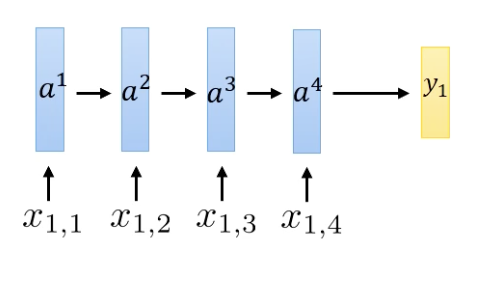
\includegraphics[scale=0.7]{images/lec11-1.png}
		\end{center}
		so, the output \( a^{3} \) hinges on the output \( a^2 \), and so on.
		For inputs with shorter length, we can just prepend a bunch of zeros, which
		does nothing to the data.
	\item In principle, this would work, but the major problem with this direct
		approach is that the number of layers in your network is equal to the length
		of the largest input. If you have very few long inputs, then the model won't
		be very good at predicting the long inputs because there isn't enough data
		out there. 

		To fix this, we tie the layer parameters together, which is called a
		recurrent neural network. It's called recurrent because each \( a^{\ell} \)
		depends recursively on \( a^{\ell - 1} \). 
	\item Something else you could do is to have an output for each input, and
		"decode" the output from that specific layer. The computation is the same,
		the only thing we've changed is that we're decoding the information at every
		step. 
	\item You could also use what's called an \textbf{autoregressive model}, which
		uses the output of the previous iteration to generate the next output. This
		is what ChatGPT does. 

		\question{How is this model different than the first one?} 

		\answer{You are getting the output at every step here, in the first type
			you're not. In other words, you're getting the output of each next word,
		which is generated based on the prevoius word.} 
	\item From this process, hopefully it's clear that there's this general setup
		going on: you have an encoder that "encodes" the input data, and a decoder
		that you run through your neural network to decode the output. That is, the
		general structure could look something like this:
		\begin{center}
			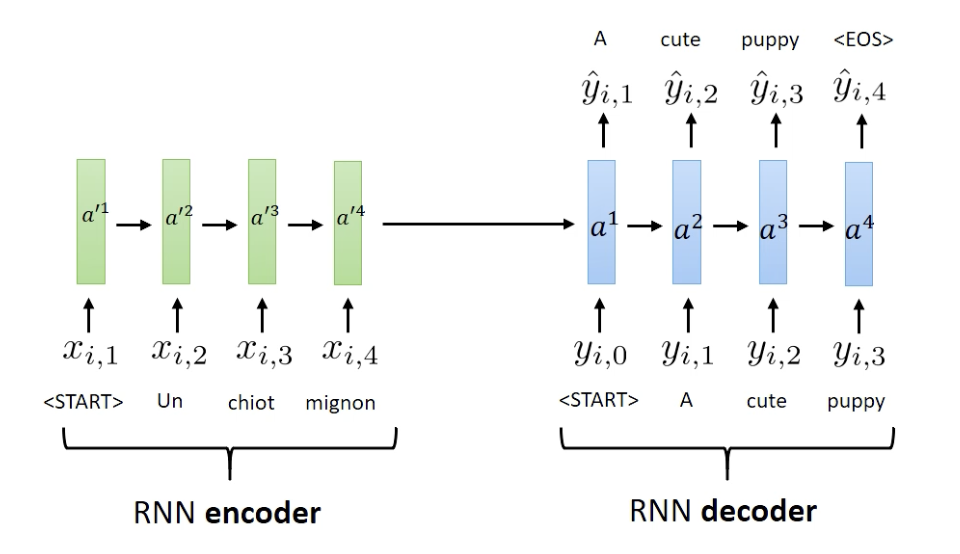
\includegraphics[scale=0.6]{images/lec11-2.png}
		\end{center}
		Note that the RNN encoder could be replaced by a CNN encoder if we were
		dealing with images. Point is, you have a neural network that
		\textit{encodes} the input data, and a decoder that \textit{decodes} the
		data. 

		The encoder translates the input into a "content vector" that describes the
		content, then the RNN decoder does the actual translation.    
\end{itemize}
\subsection{RNN Bottleneck, Attention}
\begin{itemize}
	\item One major problem with this encoder-decoder structure is the transition
		between the encoder and the decoder, called the bottleneck. In essence, if
		you have very long recurrences, then the earlier features that are passed in
		tend to get washed out the longer your recurrence goes. 

		This is the motivation for solutions that involve attention and transformers.
	\item Suppose you don't want all the information to be bottlenecked by the last
		output of the encoder, is there a way we can just translate intermediate
		outputs? The answer is yes, via attention. 
	\item Imagine the standard recurrent neural network (image below), and 
		you're trying to decode \( s_2 \). 
		\begin{center}
			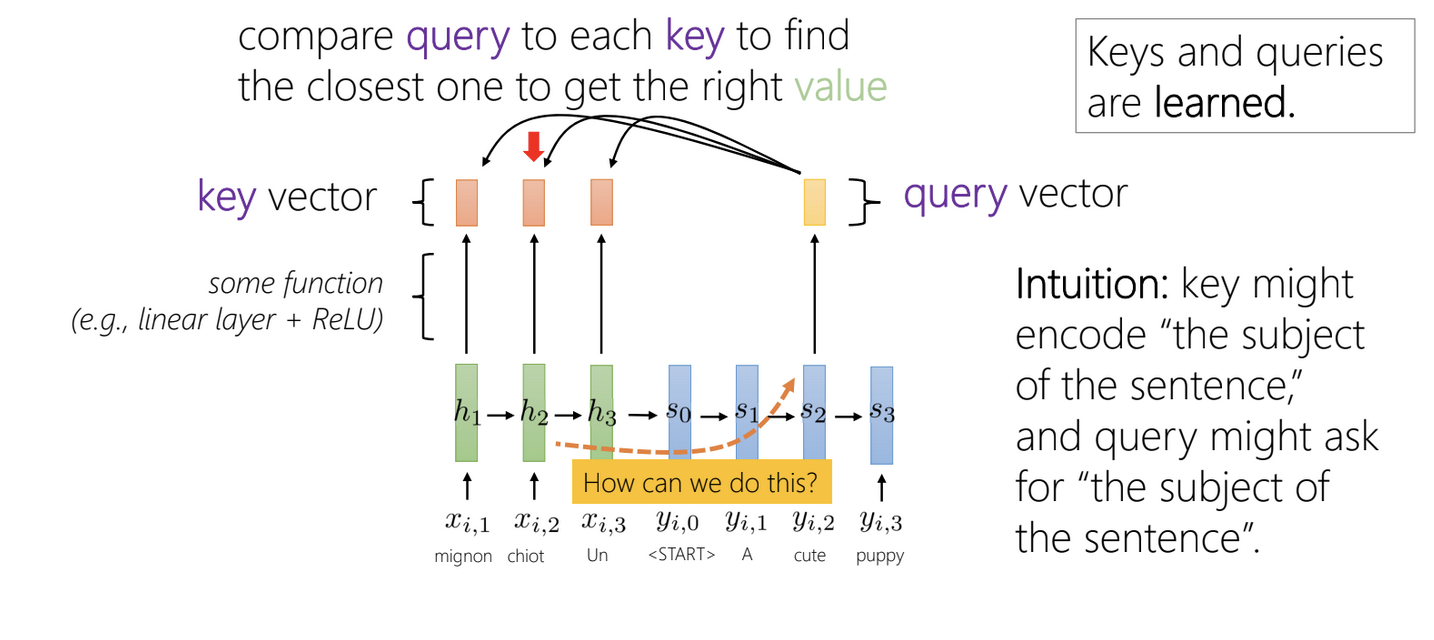
\includegraphics[scale=0.5]{images/lec11-3.png}
		\end{center}
		we can generate a query vector based on the hidden state at \( s_2 \), that
		allows us to query back in time and look for matches. This is a probabilistic
		lookup, so it picks the one that has the highest similarity, based on some
		heuristic (maybe a dot product or something).     

		\comment{The intuition to have is that if you're trying to decode the subject
			of the sentence, the query vector goes back in time and looks for the
		subject of the sentence from the encoder.}
	\item Refer to the diagram below:
		\begin{center}
			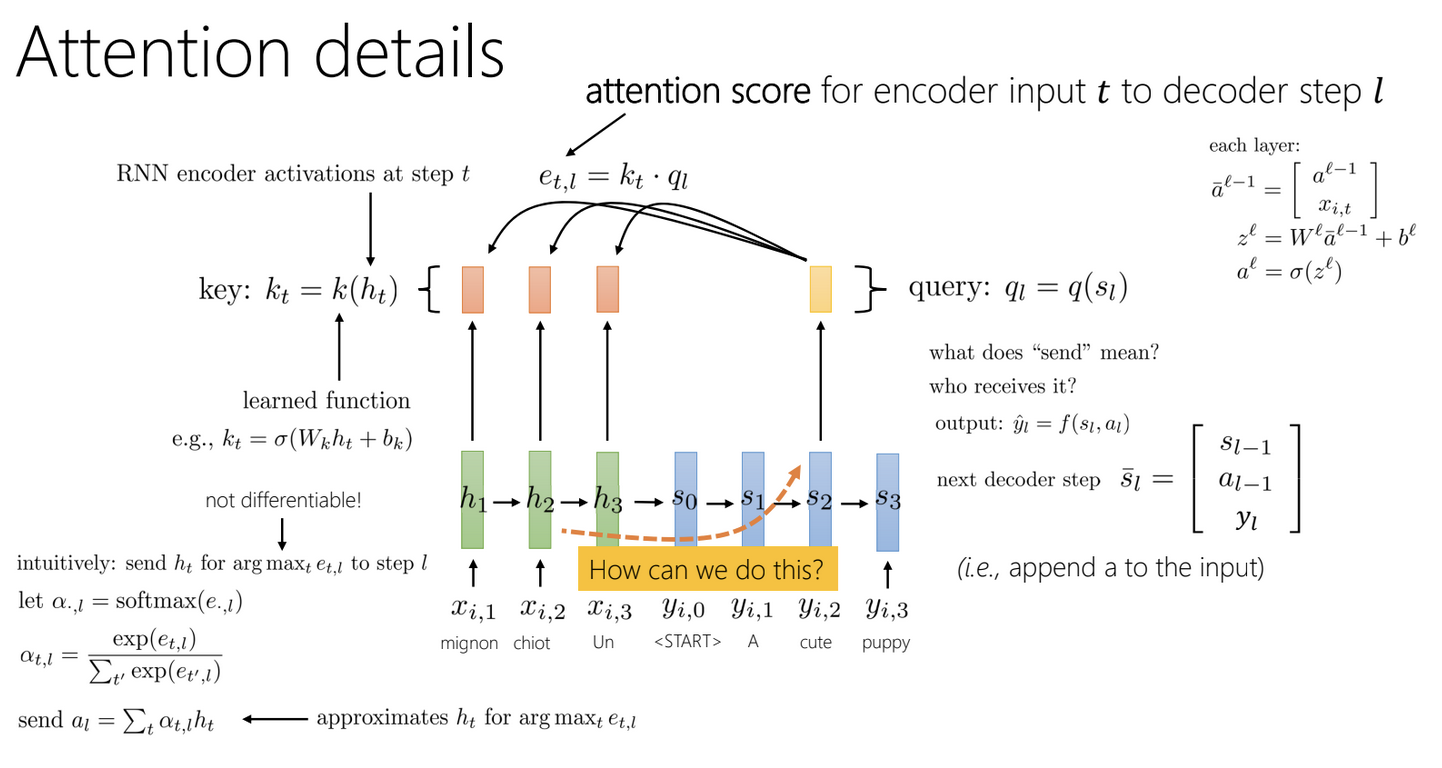
\includegraphics[scale=0.5]{images/lec11-4.png}
		\end{center}
		\begin{itemize}
			\item Suppose you're at \( s_2 \), and you're looking to query.
				To compute the keys, you take the hidden input \( h_t \) at 
				every layer, and you put it through a function \( k(h_t) \). \( k \) 
				could be as simple as the identity, but it can also be a simple 
				learned function as well (e.g. \( k_t = \sigma(W_k h_t + b_k) \)). 
			\item When you're query, you put it through a query function \( q_{l} =
				q(s_l) \). \( q_l \) is a vector representing some concept, and
				we take the inner product of \( q_l \) with every input \( k_t \).
				This quantity \( e_{t, l} \) is called the \textbf{attention score}.  
			\item Intuitively, we would like this to be a database lookup, which
				would basically be the same as looking for \( \argmax e_{t, l} \).
				But, because this is not differentiable, we normally use a softmax
				instead.  That is:
				\[
					\alpha_{t, l} = \frac{\exp(e_{t, l})}{\sum_{t'} \exp(e_{t', l})}
				\]
				Now, the combination of all of these is a normalized probability
				distribution, then we take a linear combination of the attention
				score with the information in the input sequence back. That is, we
				send \( a_l = \sum_t \alpha_{t, l} h_t \) back. Basically, this
				ensures that the things which are sent back with high probability are
				the ones that correspond highly with the data.  
			\item After sending \( a_l \) back, we can then use this information
				combined with \( s_2 \) to finally get a prediction \( \hat{y}_{2}
				\).   
			\item The number of attention scores you have depends on the length of
				the input string. The computational complexity is then dependent on
				the length of your input. 
		\end{itemize}
	\item Some general examples of \( k(t) \) and \( q(t) \) are just the identity
		function:
		\[
			k_t = h_t \quad q_l = s_l
		\]
		so the decoder is just the inner product between the encoder and decoder. You
		can also use more complicated functions, such as:
		\[
			k_t = W_k h_t \quad q_l = W_q s_l
		\]
		where \( W \) is a parameter we augment by (\question{is this learned?}). On
		the decoder side, you then have:
		\[
			e_{t, l} = h_{t}^{\top} W_k^{\top} W_q s_l = h_{t}^{\top}W_e s_l
		\]
	\item You can also do weird things with the returned \( a_l \) as well. Instead
		of just taking the dot product of the attention score with each layer, you
		can also use a learned function here, so you return
		\[
			a_l = \sum_t \alpha_t v(h_t)
		\]
		where \( v(h_t) \) is some learned function.  

		\question{We keep saying this "learned function", how do you learn functions
		like this? Do you have another neural net that does this?}
	\item Attention is a \textbf{very} powerful tool! There is no longer a bottleneck
		because each layer can just use attention. This is very similar to how
		resents work -- we're shortening the gradient path, so this makes the neural
		net better. 
\end{itemize}
\subsection{Transformers}
\begin{itemize}
	\item Is attention all we need? Do we even need the recurrence or the
		autoregressive model? The answer is no, and what we can actually do is just
		rely only on attention. This is what transformers are. 
	\item The only issue you have with the current model is that you can only look at
		the key vectors for the input pairs, but not the decoding layers. To solve
		this, we implement \textbf{self-attention}. So, we basically make a key
		vector for \textit{every layer}, including the ones in the decoding network.
	\item Refer to the following diagram:
		\begin{center}
			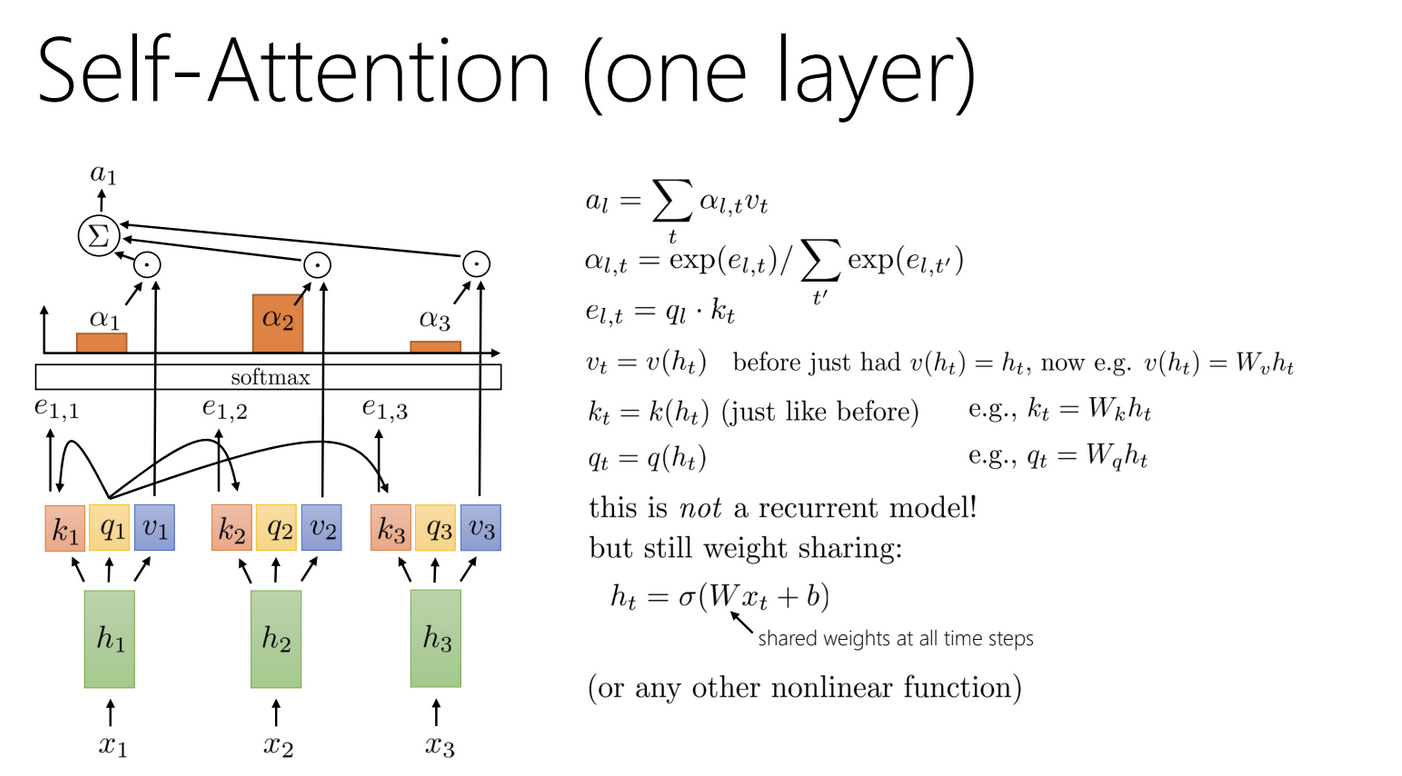
\includegraphics[scale=0.5]{images/lec11-5.png}
		\end{center}
		\begin{itemize}
			\item The intermediate arrows are now gone, and instead it's replaced by
				these \( k_i, q_i, v_i \) values. We still have a shared weight \(
				h_t = \sigma(W x_t + b) \), but they are no longer connected to each
				other. 
			\item Now, each layer has a value \( v_t \), which is defined by \(
				v(h_t) \), just as before. The key vector is also stored, in the same
				way as before \( k_t = k(h_t) \). The query is also the same as
				before. 
			\item So basically, this is a very dense version of what we had before --
				instead of having the keys in the encoder and the queries in the
				decoder, they are now all in the same system (so to speak). 
			\item If you're querying for \( h_1 \), then you query through \( k_1,
				k_2, k_3 \), and compute the attention in the same way we did before.
				The only difference is that you're querying your own key \( k_1 \) as
				well. 
			\item \( a_l \) is defined the same way, through the softmax, etc. 
		\end{itemize}
	\item Now that we've removed the recurrence, this means that the network is now
		permutation equivariant: if you switch up the order of \( h_i \) the output
		doesn't change, which is bad.  
	\item You can also stack attention layers on top of each other in the same way
		you stack a convolutional neural network. 
	\item Some issues with our model so far:
		\begin{itemize}
			\item Lack of sequence information: by removing the recurrence we've
				removed the ordering.  

				To fix this, we just force-feed position information into \( h(t) =
				f(x_t, t)\). If you just feed it in something simple (like 1, 2, 3,
				...), it actually
				doesn't do very well. What people actually do is give it a positional
				encoding \( p_t \) which is a giant vector of sines and cosines. 
			\item Multi-headed attention: in the same way you can have multiple
				kernels for your neural network, you can also have an attention layer
				for each kernel, which is called multi-headed attention.
				
				You can do multi-headed attention in parallel, the mechanisms are
				exactly the same, except in a higher dimension because we have more
				queries, keys, and values. 
			\item Linearity: each successive layer is linear in the previous one

				Fixing this just requires you to add a some nonlinear function in
				between the attention layers. 
			\item Masked decoding: How do we prevent attention lookups into the
				future?  

				This is mainly an issue caused by addressing the first issue -- when
				we bake an ordering into the system, then we have to restrict what
				each layer can query, which we can do by modifying the dot product to
				be:
				\[
					e_{l, t} = \begin{cases}
						q_l \cdot k_t & t \leq l\\
						-\infty & \text{otherwise}
					\end{cases}
				\]
				This solves the issue because now you'll get a \( -\infty \)
				attention score for the things you're not supposed to look at. 
				
				\comment{Note that throwing this into the softmax will give you \(
				e^{-\infty} = 0 \), so it does work out as expected.}
		\end{itemize}
	\item And now we've essentially built a transformer. Nowadays, transformers
		usually just refer to this stacking of self attention layers. 
	\item Some downsides is that this is pretty slow, as it runs in \( O(n^2) \),
		compared to \( O(n) \) (roughly) due to backpropagation. It's also slightly
		harder to implement. 

		That said, it also has many benefits, which outweigh the downsides: they have
		much better long-range connections, they're much easier to parallelise, and
		you can also make them much deeper than you can with RNNs.  
\end{itemize}

	\section{Dynamic Programming I}

	\subsection{Fibonacci Numbers, revisited}
	\begin{itemize}
		\item Imagine computing Fibonacci numbers; there's a lot of repeated calculations! For instance, 
			$F(1)$ is computed $2^n$ times when we're looking for $F(n)$!
		\item To optimize this, store each successive computation of $F(n)$ into an array that we access, 
			so that we only need to compute each $F(k)$ exactly once.
		\item This is called \textbf{memoization}, where we store things in a ``memo,'' to be accessed by our 
			algorithm later on. 
	\end{itemize}
	\subsection{Elements of Dynamic Programming}
	\begin{itemize}
		\item There are a couple hallmarks of DP:
			\begin{enumerate}
				\item Subproblems, or ``optimal substructure''. Refers to the fact that large problems 
					can be broken up into smaller subproblems. For Fibonacci, this means that 
					$F(n)$ is recursively expressed in terms of smaller subproblems.
				\item Overlapping subproblems: A lot of subproblems overlap with one another. We recurse to 
					smaller subproblems, and in doing so we see that a lot of computation 
					is repeated. The solution to this is to use memoization, so that 
					each computation is done only once.
		\item There are two ways to do DP:
			\begin{itemize}
				\item Top-Down: start from the largest subproblem and recurse to smaller subproblems. 
					This often involves recursion.    
				\item Bottom-up: start from the smallest subproblems then work to larger subproblems.
					Memoization still happens; we just fill the table from the small to 
					largest problems. In this method, this doesn't need a recursive call. 
			\end{itemize}
		\end{enumerate}
		\item The mathematical runtime of top-down and bottom-up are the same.
		\item The computation structure for DP actually looks awfully similar to a DAG. 
		\item If we view every subproblem as a node in the graph: construct it in such a way that 
			an edge $i \to j$ exists if the solution to subproblem $j$ directly depends on the solution to of 
			subproblem $i$. 
		\item Consider a topological sort on this DAG: then the bottom-up solution directly follows the 
			conputation of this DAG! 
			\begin{itemize}
				\item In the top-down framework, we are filling up the memo table in topological sort order, 
					since that table is still being filled from bottom up.
			\end{itemize}
	\end{itemize}
	\subsection{Shortest Paths on DAGs}
	\begin{itemize}
		\item We're given a DAG with a source $s$. We want to find the cost of the shortest path from 
			$s$ to $u$ for all $u \in V$. We also want to do this in linear time, 
			$O(n + m)$.
		\item We can always run a topological sort on this DAG in $O(n + m)$ time. Our subproblems 
			are the distances from $s$ to $u$ for every node $u$.
		\item After ordering in topological sort, we can just go down this graph \textit{in topological 
			order!} This means that the structure of the DP tree is the same as that of the topological sort.
		\item In terms of our recurrence relation, $\dist(u) = \dist(v) + \ell(u, v)$. Here, 
			$\dist(v)$ is implied to be memoized, since it's already a solved problem.
		\item This is an $O(n +m)$ solution to this problem!
	\end{itemize}
	\subsection{DP Recipe}
	\begin{enumerate}[label=\alph*)]
		\item Identify the subproblems (i.e. find the optimal substructure)
		\item Find a recursive formulation for the subproblems: just try to solve it via recursion and 
			see where it gets you.
		\item Design the DP algorithm -- fill in a table, starting with the smallest sub-problems and 
			building up. 
	\end{enumerate}
	\subsection{Shortest Paths with $k$}
	\begin{itemize}
		\item Here we consider the same problem of finding shortest path, but we're restricted to use at most 
			$k$ edges. 

			\question{Fill this out from lecture recordings}
	\end{itemize}
	\subsection{All-Pair Shortest Paths}
	\begin{itemize}
		\item Here, instead of finding the shortest path from a singular source node, we want to find 
			it for all pairs of nodes. 
		\item Input: again a graph with no negative cycles.
		\item Naively, we can run Bellman-Ford on all nodes, but this would take $O(nm)$ a total 
			of $n^2$ times, so our total runtime could be as large as $O(n^4)$ for dense graphs.
			Therefore, we're looking for a better algorithm.
		\item Identify the subproblem: subproblem $k$: for all pairs, find the shortest $u \to v$ path 
			whose internal vertices (so the path they take) only use nodes $\{1, 2, \dots, k\}$.
			\begin{itemize}
				\item In other words, there's a collection of $k$ nodes, and the path from $u \to v$ 
					\textit{only} uses these nodes.
			\end{itemize}
		\item Recursion: When we have the set from $\{1, \dots, k\}$, we want to find the relation between 
			this set and how to expand this set. There are a couple ways that the new 
			node can be added:
			\begin{itemize}
				\item Case 1: The new node added does not lie on the path: then nothing really changes, so 
					$\dist_{k +1}(u, v) = \dist_k(u, v)$.
				\item Case 2: The shortest path uses the added node: this path can be broken into two 
					parts: the shortest $u \to (k+1)$ path and then the shortest $(k+1) \to v$ path. 
					Both of these paths are already computed (by definition of them only using 
					the set $\{1, \dots, k\} $), so we just have to add these two up. 
				\item To combine these two, we find the minimum of these two to find whether the 
					path from $u$ to $v$ has changed or not.  
			\end{itemize}
		\item Runtime: Each update is $O(1)$ time, and we have to loop over $u, v$ a total of $k$ times, 
			so overall $O(n^3)$ runtime. 
		\item This is called the \textbf{Floyd-Washall Algorithm.}
	\end{itemize}

	\section{Dynamic Programming II}
	We will look more at how to choose subproblems (step 1 of our ``recipe'' to solve DP problems)
	Some problems we'll look at today:
	\begin{itemize}
		\item Longest increasing subsequence
		\item Edit distance
		\item Knapsack Problem
	\end{itemize}
	Pay attention to the information our subproblems need to be storing. 

	\subsection{Longest Increasing Subsequence}
	\begin{itemize}
		\item Given an array of integers $\left[ a_1, \dots, a_n \right]$, and we want to return the length 
			of the longest increasing subsequence of the input. (the selection of the indices \textbf{doesn't 
			have to be contiguous})
		\item We're going to deal with 1-indexed arrays here. 
		\item Why is this useful? This problem is one processing step used in a lot of other algorithms, 
			and even the game of Solitaire (also called Patience Sorting)
	\end{itemize}
	\subsubsection{Subproblems}
	\begin{itemize}
		\item Which of the following is better?
			\begin{itemize}
				\item $L[j]$ is the length of the LIS in the array $\left[ a_1, \dots, a_j \right] $ for 
					$j = 1, \dots, n$. 
				\item $L[j]$ is the length of the LIS in array $\left[ a_1, \dots, a_j \right] $ that 
					ends in $a_j$ for $j = 1, \dots, n$.

					\comment{The second one is far better, because we keep track of $a_j$ information.}
			\end{itemize}
		\item The second subproblem is better, because keeping track of $a_j$ is very valuable when we are 
			trying to recurse back in our DP problem. 

			If we don't keep track of $a_j$, we don't have any information of the last element of our 
			LIS subproblem, so we don't know how to attach it. 
		\item \textbf{Whatever the subproblem is not storing/not stating is going to be taken away from you.
			You can only observe things that the subproblem is storing/stating}
		\item To add, there are two cases:
			\begin{itemize}
				\item Suppose $a[j] \le a[i]$. Then we cannot add $a_j$ because it's not part of the 
					longest increasing subsequence. Therefore, $L[j]$ (the LIS up to $j$) is the same as 
					$L[i]$. 
				\item Otherwise, $a[j] > a[i]$, so we can add it to the LIS (so $L[j] = L[i] + 1$).
					
					\question{How is it possible that $a[j] \le a[i]$?}

					\answer{There could be an increasing sequence that grows slower that isn't counted in 
					the $i$-th iteration} 
				\item Therefore recursively, we have to apply the following:
					\begin{align*}
						L[i] &= \max_{i < j} \{L[i]: a_j > a_i\} + 1\\
						L[1] &= 1
					\end{align*}
					We want the maximum because we want the \textit{lonegest subsequence} to tack $a_j$ 
					onto.
			\end{itemize}
		\item In total, there are $O(n)$ subproblems, and each subprolbem has $O(n)$ time, so in total 
			we have an $O(n^2)$ runtime. 
	\end{itemize}

	\subsection{Edit Distance}
	\begin{itemize}
		\item Given a string $S[1, \dots, m]$ and $T[1, \dots, n]$, we want to find the smallest number of 
			edits to get us from $S$ to $T$. 
		\item Allowed operations: insert a character, delete character, change character.
		\item Why is this useful? Autocorrect, autocomplete in search engines and also DNA analysis of 
			similarities.
	\end{itemize}
	\subsubsection{Cost of Alignment} 
	\begin{itemize}
		\item Rather than thinking about distance in terms of \textit{moves}, instead we can think about 
			the cost of alignment. In other words, we look at the number of columns that don't agree.
			\begin{align*}
				&\texttt{S-NOWY} & \texttt{SN-OWY}\\
				&	\texttt{SUNN-Y} & \texttt{SUNN-Y}\\
				&\text{Alignment of cost 3} & \text{Alignment of cost 4}
			\end{align*}
	\end{itemize}
	\subsubsection{Subproblems}
	\begin{itemize}
		\item We define a 2D array to keep track of subproblems, where 
			\[
				E(i, j) = \text{EditDist}(S[1, \dots, i], T[1, \dots, j])
			\] 
			So this defines the cost of optimal alignment for strings $S[1, \dots, i]$
			into $T\left[ 1, \dots j \right] $.
		\item What are the different ways we can align the subproblems?
			\begin{itemize}
				\item $S[i]$ is dangling, $T[j]$ is dangling, $S[i]$ and $T[j]$ are both fully aligned. 
					Visually:
					\begin{center}
						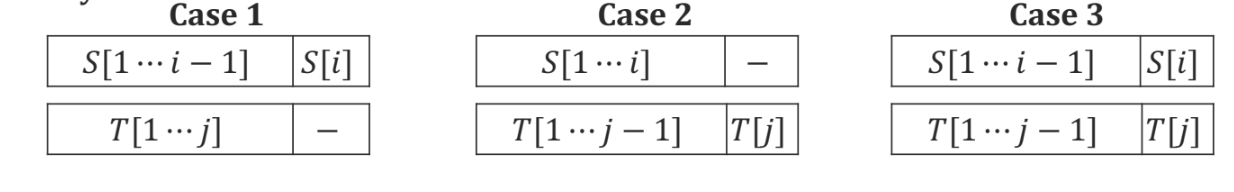
\includegraphics[scale=0.5]{alignment.png}
					\end{center}
					\comment{We add in one at a time, so there can only be one dangling letter (or none) 
					at a time!} 
			\end{itemize}
		\item We recurse based on the cases:
			\begin{itemize}
				\item Case 1: $S(i, j) = S(i-1, j) + 1$.
				\item Case 2: $S(i, j) = S(i, j-1) + 1$. 
				\item Case 3: $S(i, j) = S(i-1, j-1) + 1(S[i] \neq T[j])$.
				\item Base cases: $S(i, 0) = i$, $S(0, j) = j$. 

				The 1 represents an indicator function that counts the number of misaligned characters.
			\end{itemize}
		\item During the recursion step, we want to fill $S(i, j)$ with the \textit{minimum} value 
			of these three, since we want to minimize the number of edits. We will store this information 
			(memoizing) in a 2D array.
		\item We have to traverse our array either row by row, column by column, or diagonally. This is because
			we need to ensure that all three subproblems that we're considering have already been 
			computed. 
		\item Pseudocode:
			\begin{center}
				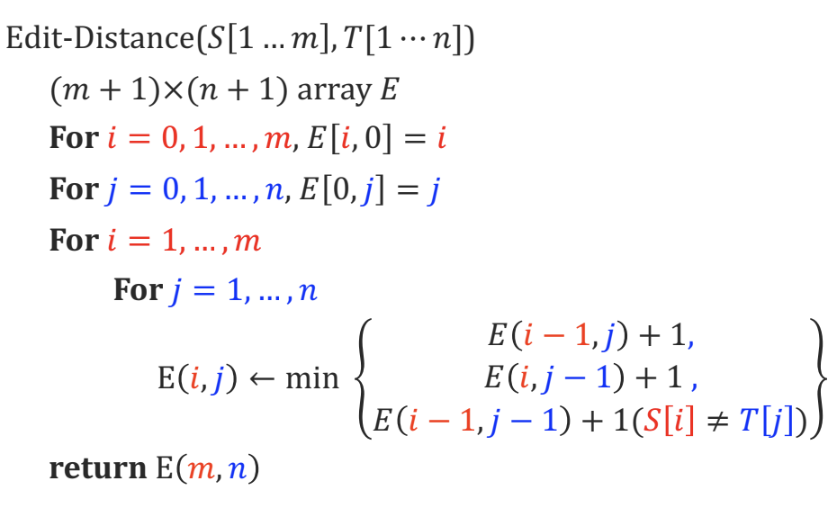
\includegraphics[scale=0.5]{alignment-pseudocode.png}
			\end{center}
		\item Runtime: there are $O(mn)$ subproblems, since we have a 2D array of dimension $mn$. At each 
			subproblem, we are only computing a minimum, which is $O(1)$ runtime, so we just have 
			$O(mn)$ runtime. 
			
			\question{Isn't the indicator also computed at this step? Why is that not accounted in the runtime?}

			\answer{The indicator is run in constant time, since we're only looking at the $i$-th character 
			in comparison to the $j$-th character.}
	\end{itemize}
	\subsection{Knapsack (with repetition)}
	\begin{itemize}
		\item A weight capacity $W$ and $n$ items with weights and values $(w_i, v_i)$. We want to output
			the most valuable collection of items whose total weight is at most $W$.
		\item We will be selecting with repetition here, but there is an easier variation where we don't
			consider repetition.
	\end{itemize}
	\subsubsection{Subproblems}
	\begin{itemize}
		\item For all $c \le W$, we want to consider the best achievable arrangement for knapsack of 
			capacity $c$. 
		\item Recurrence: For a given item $i$, then once we put it in the knapsack there are only $
			c - w_i$ capacity that remains to be optimized. This is our recurrence relation.
			\[
				K(c) = \max_{i : w_i \le c}\{v_i + K(c - w_i)\} 
			\] 
			This is a maximum over the value because we want to maximize the value being put in our 
			knapsack.
		\item We will store this information in an array of size $W + 1$, since we need a $K(0)$ element.
			\begin{center}
				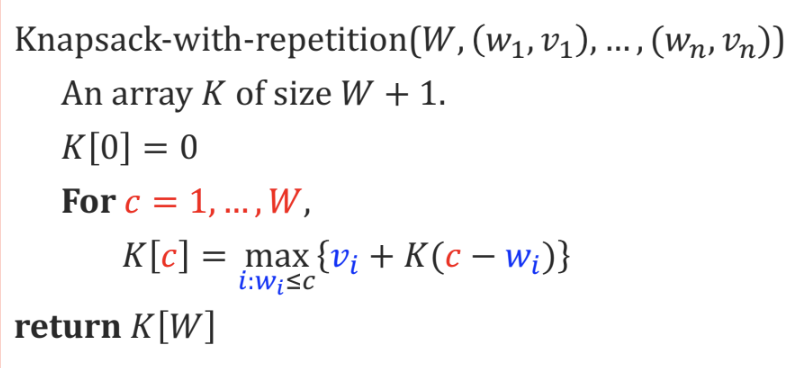
\includegraphics[scale=0.5]{knapsack-repetition.png}
			\end{center}
		\item Runtime: There are $O(W)$ subproblems, and at each subproblem, we have maximally $n$ items
			 we need to check. So in total, we have $O(nW)$ runtime.
		 \item Generally we want to think of the runtime in terms of the input. For graph problems, we looked 
			 at the input size $|V|$ and $|E|$. But for this problem, $W$ takes $\log(W)$ bits to represent 
			 $W$. So the input size is $\log(W)$. For the weights of the items themselves,
			they also only have at most $\log(W)$ bits, Therefore, the total runtime is $O(n \log W)$. 

			This kind of algorithm is polynomial in $n$, but not $W$. This is called a \underline{pseudo-
			polynomial} algorithm, since it's an algorithm that's polynomial given the numerical value 
			of the input but not in the input size.
	\end{itemize}

	\section{Dynamic Programming III}

We'll look at more examples today of DP.

\subsection{Knapsack (without repetition)}
\begin{itemize}
	\item Start with a recap with knapsack: had a weight capacity $W$, and a set of items with individual 
		weights $(w_i, v_i)$, and we wanted to look at the most valuable combination of items.
	\item Now, we're going to look at this problem with the with the constraint that \textit{we cannot 
		choose with repetition}
	\item To solve, look at how we solved the problem with repetition: introduced $K(c)$ which gets us 
		the best achieveable value for a capacity $c \le W$. The issue with trying the same thing 
		is that our subproblems don't track which items have already been used. Why not keep track of both? 
\end{itemize}

\subsubsection{Subproblems}
\begin{itemize}
	\item Introduce a 2D array: essentially solve the problem for smaller knapsacks and also smaller 
		capacities. Then expand in two directions: in terms of the number of items and also the 
		capacity.
	\item So keep track of all weights $c \le W$ and all items $j \le n$. Define $K(j, c)$ to be the 
		optimal solution to the knapsack for capacity $c$ and items $\{1, 2, \dots, j\} $. (It doesn't 
		need to use all the items from 1 to $j$.
	\item For each $K(j, c)$, we recurse smaller subproblems:

		\textit{Case 1:} The optimal solution on items 1 through $j$ doesn't use item $j$. 
					Here, $K(j, c) = K(j-1, c)$.

			\comment{Note that this is not equivalent to $K(j-1, c - w_j)$, since the $w_j$ could be 
			distributed among other items.}

		\textit{Case 2:} the optimal solution on items 1 through $j$ uses item $j$.
		Here, $K(j, c) = K(j-1, c - w_j) + v_j$. We add $v_j$ to $K$ since we're now using item $j$.   

		The intuition here is that we use the optimal solution without item $j$, then add in item $j$ 
		at the end. 
\end{itemize}
\subsubsection{Implementation}
\begin{itemize}
	\item So let's formalize this:
		\[
			K(j, c) = \max\{ K(j-1, c), v_j + K(j-1, c - w_j)\}
		.\]
		with base cases $K(0, c) = 0$ and $K(j, 0) = 0$. The base cases make sense since with no items our 
		optimal value is 0, and with no allowed weights then the optimal value is also 0. 

	\item Looking at $K(j, c)$ it only relies on the subproblmes $K(j-1, c)$, or $K(j-1, c - w_j)$, so we're 
		only looking at row $j-1$, and different elements in that row. This tells us about the order in which 
		we should be solving the subproblems: we could either do this row by row or column by column. 
	\item For runtime, ther eare $O(nW)$ subproblems, and in each subproblem we're doing constant 
		work (memory access), so therefore the total runtime is $O(nW)$, just like knapsack with repetition. 
	\item For space complexity, notice that each $K$ only depends on the previous row, so once we've 
		moved onto the 3rd row, we no longer need the first. We can delete this from memory, so the optimized 
		space complexity is $O(W)$. 
\end{itemize}
\subsection{Traveling Salesperson Problem}
\begin{itemize}
	\item A notoriously difficult problem, and DP helps us get a \textit{slightly} better runtime. 
	\item Input: Cities $1, \dots, n$ and pairwise distances $d_{ij}$ between cities $i$ and $j$. We want to 
		find a ``tour'' of minimum total distance (so we need to visit every city exactly once and 
		return to the city we started at).
	\item The naive brute-force algorithm basically is the one where we have to go through all possible 
		tours: there are \( n! \in O(n^n) \) possible tours, which makes this computation very expensive. 
	\item Dynamic programming gives us $O(n^2 2^n)$. (this is nearly optimal, beating $O(n 2^n)$ is theorized
		to be impossible)
		\begin{itemize}
			\item To give an illustration of the difference DP makes, if $n = 25$, then $O(n!) \approx 10^{25}$, 
				whereas $O(n^2 2^n) \approx 10^{10}$, so we're already better by 15 orders of magnitude. 
		\end{itemize}
\end{itemize}
\subsubsection{Subproblems}
\begin{itemize}
	\item One challenge of TSP is that subproblems aren't exactly solving the problem. If we just look at 
		TSP for a subset of our graph, that doesn't necessarily give us a solution to the larger problem, since 
		we're looking for cycles. Instead, we think of ``partial solutions'' to our graph. 
	\item We think of the subproblmes as starting from city 1, ends in city $j$, and passes thorugh all cities
		in a set $S$ (which includes city 1 and \( j \)). Visually:
		\[
			1 \to i_1 \to i_2 \to \dots \to j			
		\]
		So we want to formally define $T(S, j)$ to be the length of the shortest path visiting 
		all cities in $S$ exactly once, starting from 1 and ending at $j$. 
\end{itemize}
\subsubsection{Recurrence Relation}
\begin{itemize}
	\item How to compute $T(S, j)$ using smaller subproblems? Well, look at the string again:
		\[
			\overbrace{\underbrace{1 \to i_1 \to i_2 \to \dots \to i}_{T(S \setminus j, i)} \to j}^{T(S, j)}
		\]
		To actually talk about $T(S, j)$, then we need to add $d_{ij}$ onto every $T(S \setminus j, i)$. However,
		what is annoying is that we actually don't know which city is second to last, so we'll need 
		to consider every possible city $S \setminus j$. 
	\item So, we'll have to pick the minimum over all $i \in S$ such that $i \neq j$. Formally:
		\[
			T(S, j) = \min \{T(S \setminus j, i) + d_{ij} | i \in S \land i \neq  j\} 
		\]
	\item Our base cases are $T(\{1\} , 1) = 0$, this is fairly trivial. We also want that $T(S, 1) = \infty$.
		The reason we want this is because we're talking about incomplete paths, so $T(S, 1)$ is not 
		a valid non-cycle. Hence, we want to set it to $\infty$.  
	\item We're not done though, because we have to do something to get us back to a cycle! At the end of 
		the recursion step, we'll want to add the final edge $(j, 1)$ back, but adding only the minimum:
		\[
			T(S, 1) = \min_{j \neq  1}\{T(\{1, \dots, n\}, j) + d_{j 1}\}
		\] 
\end{itemize}
\subsubsection{Implementation}
\begin{itemize}
	\item Want an array of size $2^n \times n$, and start with base cases. Then work on the recursion:
		\begin{center}
			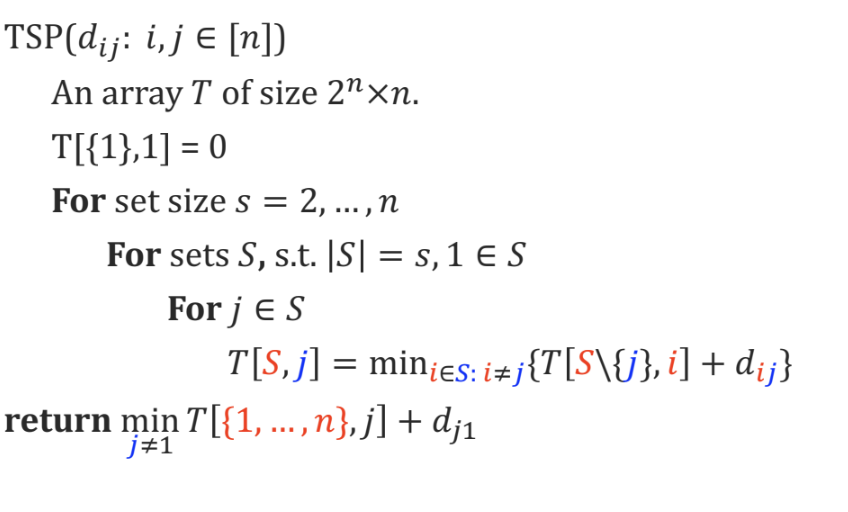
\includegraphics[scale=0.5]{TSP-code.png}
		\end{center}
	\item For runtime, there are $O(2^n \times n)$ subproblems, and on each layer we're doing $O(n)$ work, since
		we're checking the minimum across $n$ nodes every iteration. So, we have $O(n^2 2^n)$ as 
		the final runtime. 

		\question{How do we explain that \(n^2 2^n\) is the number of subproblems?}

		\answer{$O(n)$ work at every step, then $n \times 2^n$ subproblems. There are $2^n$ subsets, and in 
			each subset we can choose a $j$ to exclude, which we can upper bound by saying that there are $n$ 
		of these. So $n \times 2^n$ is a tight upper bound on the number of subproblems.}
\end{itemize}
\subsection{Independent Sets in Trees}
\begin{itemize}
	\item We're given an undirected graph \(G = (V, E)\), and want to output the largest independent 
		set of \(G\).
	\item Recall that a set \(S \subseteq V\) is considered independent if there are no 
		edges between \(u, v \in S\).
	\item This is also a notoriously hard problem, for general graphs. There isn't a polynomial time algorithm 
		that does this. But for trees, we're in luck!

		\question{Why isn't the solution just selecting every other layer?} 

		\answer{There are instances where we can pick from two consecutive layers and still not have an edge. 
		Consider the tree:
			\begin{center}
				\begin{tikzpicture}
					  \node {A}
					child {node {B}}
					child {node {C}}
					child {node {D}
					  child {node {E}}
					  child {node {F}}
					};
				\end{tikzpicture}
			\end{center}
			Our greedy algorithm would select either \(\{A, E, F\} \) or \( \{ B,C,D\} \), but the optimal set
			is actually 
		\(\{B, C, E, F\} \), so this proves that our algorithm isn't optimal.}
	\item For trees, we know that they don't have cycles, so we can pick any node and say that that is the root.
		By doing this, we can get a ``natural ordering'' of the subproblems. 
\end{itemize}

\subsubsection{Subproblems}
\begin{itemize}
	\item Let \(I(v)\) be the size of the maximum independent set in the subtree that is rooted at \(v\). 
	\item Why is this a good subproblem? Becuase it's easy to write a recursion relation for it!
	\item For the subproblems, there are two cases:

		\textit{Case 1:} \(v\) (the root of the tree) is part of the optimal independent set. This 
		means that the children aren't allowed to be part of the independent set. So if we take $v$, we can't 
		take any of the subproblems. So we need to look instead at the \textit{grandchildren} of \(v\) to join.
		Here, we'd write this as:
		\[
			I(v) = 1 + \sum_{u\  \in \text{ grandchildren}} I(u)
		\] 
		We add 1 here because we're including \(v\) now. 

		\textit{Case 2:} \( v\) is not part of the optimal independent set. Here, we would just take 
		the maximum of the children. Then:
		\[
			I(v) = \max_{u \ \in \text{ children}} \{I(u)\} 
		\] 


		So we'll take the max of these two cases:
		\[
		I(v) = \max \{1 + \sum_{u \ \in \text{ grandchildren}} I(u), \sum_{u \ \in \text{ children}} I(u)\}
		\] 
		Also, base cases is that $I(\text{leaf}) = 1$. 
\end{itemize}
\subsubsection{Implementation}
\begin{itemize}
	\item We need a data structure to store the tree easily, and also make sure that every child is processed 
		before the parents are. Well, we can iterate through the graph in post decreasing post order! 
	\item The runtime of DFS on trees is \(O(|V|)\), and each edge is looked at \(\le 2\) times -- once 
		for the children and also once for its grandchildren, so each subproblme takes constant time. 
	\item So that the total work is \(O(|E|) = O(|V|)\), since \(|E| = |V| - 1\).
\end{itemize}

	\section{Nearest Neighbor and Metric Learning}
\subsection{Parametric vs. Non-Parametric Models}
\begin{itemize}
	\item So far, we've mostly focused on parametric models, where we aim to learn \( p(y \mid x) \), through
		the use of a parameter \( \theta \):
		\[
			p_{\theta}(y \mid x) \approx p(y \mid x)
		\]
	\item The parameters are determined through MLE (or some other method), and generally the data is then
		thrown away. Today, we will look at non-parametric models (i.e. models which don't consider a
		parameter \( \theta \)). In this case, we will keep the training examples, and in effect the number
		of training parameters grows with \( n = |\mathcal{D}| \). In some sense, the dataset itself is the
		parameters. 
	\item As an aside, we should cover metric spaces first: a metric space is a set \( X \) together with a
		notion of distance \( d \) between its elements:
		\begin{enumerate}[label=\arabic*.]
			\item \( d(x, x) = 0 \).
			\item \( d(x_1, x_2) > 0 \) if \( x_1 \neq x_2 \).
			\item \( d(x_1, x_2) = d(x_2, x_1) \).
			\item Triangle inequality. 
		\end{enumerate}
		One metric we commonly see in ML is called the \textit{Mahalanobis distance}, written as:
		\[
			d_M(x_1, x_2) = \sqrt{(x_1 - x_2)^{\top} M (x_1 - x_2)}
		\]
		this collapses to the Euclidean distance when \( M = I_d \).
\end{itemize}
\subsection{KNN Classifier}
\begin{itemize}
	\item Suppose you've classified some data into two classes, and now you want to classify a new point \( x
		\). To do this, we first find the \( K \) closest (using a metric \( d \)) examples in the
		pre-existing data to inform our decision on what \( x \) should be classified as. We denote this set
		as \( N_K(x, \mathcal{D}) \). 

		\question{How is the pre-existing data generated?} 
	\item We then look at the labels \( y_i \) for the points \( N_K(x, \mathcal{D}) \), and use it to
		estimate what \( p(y \mid x)  \) should be (i.e. what label we assign it):
		\[
			p(y = c \mid x, \mathcal{D}) = \frac{1}{K}\sum_{i \in N_k(x, \mathcal{D})} I[Y_i = c]
		\]
		note that this probability sums to 1 when we sum over all \( c \), so this is actually a valid
		probability distribution. In words, this means that the probability a point \( y \) is assigned a
		label \( c \) is given by the proportion of the nearest \( K \) points that are assigned \( c \).
	\item The \( k = 1 \) case is special - the partition that you get is called a \textit{Voronoi
		tessellation}. In this case, if you scatter some points onto the plane, then this division will
		partition the space up strictly based on distance and all the boundaries are just straight edges
		between classes.  

		In this special case, the classification of a new point is given by the nearest neighbor, so this is
		why you get such a special pattern.

		\question{How do you tell the classifier how many classes you should make?} 

		\answer{This is probably something you decide ahead of time; there's probably no way for you to
		"train" a model to know how many you should make.}
	\item Visually, you can also compare different \( K \) and \( K' \) nearest neighbor algorithms, and
		there is a distinction between them. For larger \( K \), the general trend is that the boundary
		between classes gets finer and not as jagged, as is typically seen in a smaller \( K \).  
	\item There is also an optimal \( K \) for classification. If \( K \) is too large, then you risk
		comparing against points that are not near your target point \( y \), and therefore you will get a
		bad classification from it. 

		This is also a general trend we observe in model training: as the model complexity increases, the
		training error decreases monotonically, but the test error reaches an optimum somewhere in between.
		This is because there are two regimes on the extremes: extreme simplicity on one end, and overfitting
		on the other. 
\end{itemize}

\subsection{KNN Generative Classifier}
\begin{itemize}
	\item Now we move to the \( K \)-nearest neighbors except this time we have a generative classifier. In
		this case, we essentially define a "ball" around each point \( x \) until we encounter \( K \)
		points, and the classification is then given by the proportion of points in that ball \( V_K(x) \)
		that are classified as class \( c \).      
	\item If you have a \textit{lot} of data, it has been shown that the KNN test error can never be worse
		than twice the optimal Bayes classifier. This is interesting to note, because the Bayes classifier
		requires \textit{much} more information about your data (the class conditionals, distribution, etc.),
		but KNN knows nearly nothing.  
	\item This is a quick aside, but basically the idea is that the space you need to check increases
		exponentially with dimension. Because the volume grows exponentially large, it becomes increasingly
		more impractical to search such a space, and so this makes KNN much worse in higher dimensions.  

		If you want to get \( \epsilon \) close to a target, by increasing the dimension you can only get 
		\( O(n^{ - 1 / d}) \) closer to the target by increasing the dimension. 
\end{itemize}

\subsection{Pros and Cons of KNN}
\begin{itemize}
	\item Pros:
		\begin{itemize}
			\item Fast, no training required.
			\item Learns complex classification functions easily, because it requires no priors.
		\end{itemize}
	\item Cons:
		\begin{itemize}
			\item High storage cost
			\item Slow at computing inference (actually performing the classification)  
			\item Very bad dimensionality scaling. 
		\end{itemize}
\end{itemize}

\subsection{Manifold Hypothesis}
\begin{itemize}
	\item The manifold hypothesis basically states that "true" high dimensional data that we care about, like
		images, videos, etc. lie in a lower dimensional manifold which is embedded in a higher dimensional
		space.   
	\item The idea then is that we essentially "embed" the data onto a lower dimensional space using a neural
		network, learn the
		space using a Euclidean metric, then you can classify using this Euclidean metric. 

		\question{Is this the approach that t-SNE uses?}
	\item The challenge then becomes: how do you define an embedding that does exactly what you want?
		Ideally, you want an embedding that pulls similar objects close to each other and pushes dissimilar
		ones apart.
	\item One of the earliest approaches to doing this was based on \textit{contrastive loss}. Basically,
		define a loss function over two points \( i, j \):
		\[
			\mathcal{L}_{ij}(\theta; m) = \mathbb I (y_i = y_j)d(z_{\theta}(x_i), z_{\theta}(x_j))^2
			+ \mathbb I (y_i \neq y_j) \max(0, m - d(z_{\theta}(x_i), z_{\theta}(x_j))^2)
		\]
		(recall that \( z(x) \) is your embedding function). 
		Essentially, you minimize the loss between similar points, while also defining a "maximum acceptable
		distance" between two dissimilar points. You require this \( m \) because otherwise, your model will
		want to push dissimilar points increasingly farther away off to infinity.  

		Tested this on the MNIST dataset and bringing this down to a 2-dimensions from 784 dimensions, and
		the results look very good.    
	\item The problem with this approach is that the "pull" and "push" terms don't talk to each other, or in
		other words this is a very binary way to approach this embedding approach. 
	\item This leads to the second approach: triplet loss. Here, the loss is given by:
		\[
			\mathcal{L}_i(\theta; m) = \max(d(z_\theta(x_i), z_{\theta}(x_i^{+}))^2 - d(z_{\theta}(x_i),
			z_{\theta}(x_i^{-}))^2 + m, 0)
		\]
		In essence this does the exact same thing: you want the first term to decrease while simultaneously
		wanting the second term to increase, but this is a more clever approach because the terms are
		combined together. 
		
		Here, \( z^{+} \) is a positive (similar) example, and \( z^{-} \) is a dissimilar (negative)
		example.  

		\question{what is the positive and negative example referring to?} 

		\answer{these are \textit{anchors} in the data, and are given as true points in the dataset.}  
	\item One issue with the triplet loss is that because there are a lot of negative examples to compare to,
		you naturally need to perform that computation many many times to get the loss for a single point.
		This leads to the \( N \)-pair loss, which lets you take a batch of negaitve samples at a time:
		\[
			\mathcal{L}(\theta; x, x^{+}, \{x_k^{-}\}_{k = 1}^{N}) = \log\left( 1 + \sum_{k = 1}^{N -
			1}\exp\left( \hat{z}_\theta(x)^{\top} \hat{z}_\theta(x_k^{-}) - \hat{z}_\theta(x)^{\top}
			\hat{z}_\theta (x^{+}) \right) \right)
		\]
		what this means is that you take a set of predefined dissimilar examples \( \{x_k\} \) and use that
		as the "push" term. 

		\question{How does this algorithm work in practice? Would you have to define a set of similar and
		dissimilar classes for every class you're working with?} 

		\comment{The reason you don't need a max function here is because \( \hat{z}_\theta(x) \) is a
			projection that only projects into a volume of a unit sphere, so there is a predefined limit to
			how far apart dissimilar points can be apart. You can also convert this interpretation into an
		equivalent one using softmax.}   
	\item There's also the world of joint embeddings: where text and images are encoded together and embedded
		onto a space: OpenAI's CLIP model was trained on an \( N \)-pair loss in a jointly embedded space.  
\end{itemize}

	\section{Network Flow}
\begin{itemize}
	\item Recently declassified (1999) document about the USSR's shipment capacity from east to west. This 
		was crucial information at the time since had a war broke out, the US could identify which 
		supply routes they could bomb.
	\item They devised a greedy algorithm called ``flooding,'' but this algorithm wasn't really optimal. It 
		was finally solved by Ford and Fulkersson, and is now called the Ford-Fulkersson algorithm.
	\item Given a directed graph $G = (V, E)$, one source vertex $s$ and a sink $t$, and for each edge $e \in E$,
		we're given a capacity $c_e$ which are integers. 
	\item We want to find the maximum amount of water from $s \to t$.  
	\item \textit{Definition:} A flow assigns a number $f_e$ to each directed edge $e \in E$ such that:
		\begin{itemize}
			\item nonnegativity: \(f_e \ge  0\) 
			\item capacity: \(f_e \le c_e\)
			\item flow in and flow out are equal: \(\sum_{u \to v} f_{u, v} = \sum_{v \to w} f_{v, w} \)
		\end{itemize}
	\item Let's also define the size of the flow $f$ to be the total quantity set from $s$ to $t$. Using 
		this definition, then the maximum flow is the one that maximizes $\size(f)$. This can be solved 
		using linear programming!
\end{itemize}

\subsection{Greedy (suboptimal) algorithm}
\begin{itemize}
	\item We'll find a path $P$ from $s$ to $t$, and send flow until it's saturated. We'll do 
		this as much as we can. We repeat this until we run out of paths.
	\item This algorithm fails on some graphs, because it uses edge $A \to B$ when that edge is suboptimal! 
		Consider the graph:
		\begin{center}
			\begin{tikzpicture}[scale=2]
				\node (s) at (0, 0) {$s$};
				\node (a) at (1, 0.7) {$A$};
				\node (b) at (1, -0.7) {$B$};
				\node (t) at (2, 0) {$t$};
				\graph[edge label = 1]{(s) ->(a) -> (t), (s) -> (b) -> (t), (a) -> (b)};
			\end{tikzpicture}
		\end{center}
		Our algorithm just looks at flow rate, so a possible path to take is $s \to A \to B \to t$, but this 
		is clearly suboptimal! Instead, we should be going from $s \to A \to t$ and $s \to B \to t$. 
\end{itemize}

\subsection{Greedy Fix}
\begin{itemize}
	\item We instead consider a residual graph, where we subtract the flow given by greedy 
		($s \to A \to B \to t$), and also generate a back edge that travels in the reverse order of the flow 
		given by greedy, so that we can backtrack if needed. 
	\item Formally, given a graph $G$ and a flow $f$ on $G$, the residual raph $G_f$ is defined as:
		For all edges \((u, v)\), if $f$ goes from $u \to v$, then the residual graph will flow from $v \to u$ 
		and the edge will have capacity $c_{u, v} - f_{u, v}$. 

		By doing this, we allow our graph to backtrack along our suboptimal path if needed.  
	\item This is the approach that Ford Fulkerson uses to find the optimal flow.
\end{itemize}

\subsection{Ford-Fulkerson Algorithm}
\begin{itemize}
	\item Find a path $P$ from $s$ to $t$ in the residual graph which is not yet saturated, and send more 
		flow along $P$. We keep repeating this until everything's saturated, and this happens 
		when all edges along one particular cut is zero. 
	\item To show that this algorithm terminates, lets' first define an $s-t$ cut is a partition of the graph
		into two sets of vertices \(L\) and \( R\) such that 
		\(s \in L\) and \(t \in R\). We define the capacity of this cut to be the sum of all capacities from 
		the edges that cross from $L$ to $R$.  
	\item Therefore, for any flow $f$ and any cut \((L, R)\), then \(\size(f) \le \capacity(L, R)\). Then, the
		flow is actually upper bounded by the minimum cut along this graph (this is our ``bottleneck'' introduced
		at the outset)
	\item Then, this means that the max flow is also given by the minimum cut, and we can show that 
		Ford-Fulkerson outputs a maximum flow by considering this relation between the flow and a cut. The proof 
		of this is outlined in lecture. 

		\question{Review the proof for this later}
\end{itemize}

\subsection{Runtime}
\begin{itemize}
	\item The number of augmenting paths must be less than $U$, where $U$ denotes the maximum flow, so 
		the update is less than $O(m + n) \cdot U$. 
	\item But what this means   
	\item There are other algorithms out there that optimizes this a little more: Edmonds-Karp gives 
		us a runtime of $O(n m^2)$, which is much better than what we have. 
	\item The best runtime was discovered last year, where we have $O(m^{1 + o(1)} \cdot \log U)$
\end{itemize}

	\section{Laplace Transform}
\begin{itemize}
	\item Laplace transforms concern the equation:
		\[:tabn
		X(s) = \int_{-\infty}^{\infty} x(t) e^{-st} \diff t
		\] 
		The basic idea is that instead of solving for \( x(t) \), we solve instead for \( X(s) \), which is 
		much easier to do sometimes than \( x(t) \). 
	\item Suppose you have an LTI system with impulse response \( h(t) \), and we input a harmonic 
		exponential \( e^{j 2\pi ft} \), then we get an output \( y(t) = H(f) e^{j 2 \pi ft}
		= H(\omega) e^{j \omega t}\). (this is the 
		eigenfunction property.)
	\item What about an input \( e^{st} \)? Then, we can express this as a convolution, which 
		happens to be written as: \( y(t) = H(s) e^{st} \), where  \( H(s) \) is the Laplace transform of 
		\( h(t) \). 
	\item Consider an input \( x(t) = e^{st} \), and since \( s \in \C \), then we can write 
		\( s = \sigma + j \omega \). Then we convolve:
		\[
		y(t) = \int_{-\infty}^{\infty} h(t) e^{s(t - \tau)}\diff \tau = \int_{-\infty}^{\infty} 
		h(t) e^{st} e^{-s \tau}\diff \tau = e^{st}\underbrace{\int_{-\infty}^{\infty} h(\tau) e^{-s \tau}\diff \tau}
		_{H(s)}
		\] 
		where the integral we defined earlier as the Laplace transform \( H(s) \). Here, we call it 
		specifically the bilateral Laplace transform of \( h(t) \). This distinction just has to do with the 
		integration bounds; a unilateral Laplace transform is defined as 
		\[
		H_{\text{uni}}(s) = \int_{0}^{\infty} h(\tau)e^{-s \tau}\diff \tau 
		\] 
		but we will normally consider bilateral Laplace transforms in this class.  
	\item Note also that the Laplace transform is also the more general case of the Fourier transform: the Fourier
		transform occurs when \( \Re(s) = 0 \). 
\end{itemize}
\subsection{Notation, Terms}
\begin{itemize}
	\item With Laplace transforms, we say that they transform between the time domain and the \( s \)-domain, and 
		it's written as:
		\[
		\mathcal L \{x(t)\}  = X(s) = \int_{-\infty}^{\infty} x(t) e^{-st}\diff t 
		\] 
		Because \( s \) is a complex number, the Laplace transform takes our 1-dimensional signal 
		\( x(t) \) and turns it into a two-dimensional signal in  \( s\)-space. 
%		\begin{center}
%			\begin{tikzpicture}
%				\draw (-3, 0) -- node[right] {\( t \) } (3, 0);
%			\end{tikzpicture}
%			\( \rightarrow \) 
%			\begin{tikzpicture}
%				\draw(-3, 0) -- (3, 0) node[right] {Real};
%				\draw (0, -3) -- (0, 3) node[left] {Imaginary};
%				\draw[red] (0, 0) -- node[right] {\( X(s) \) } (1, 2);
%			\end{tikzpicture}
%		\end{center}
\end{itemize}
\subsection{Laplace Transform Pairs}
\begin{itemize}
	\item Given a signal \( x(t) = \delta(t) \), then the Laplace transform \( X(s) = 1 \). This is seen easily 
		from the integral itself:
		\[
		X(s) = \int_{-\infty}^{\infty} \delta(t) e^{- st}\diff t = 1 
		\] 
		As a 2D diagram, we can imagine that over the entire complex plane, \( X(s) \) takes on a value 
		of 1. 
	\item Given a unit step function \( x(t) = u(t) \), then the Laplace transform \( X(s) = \frac{1}{s} \). 
		Again, just do the integral:
		\[
		X(s) = \int_{-\infty}^{\infty} u(t) e^{-st}\diff t = \int_{0}^{\infty} e^{-st}\diff t = \frac{1}{s} 
		\] 
		Note that this only works if \( \Re(s) > 0 \), otherwise we have an unbounded integral. This condition 
		is also called the \textit{region of convergence} for the integral. This actually means that 
		the Laplace transform may not be defined for all values of \( s \)!

		\comment{Note that \( \Im(s) \) doesn't matter here, since all it does is give us an overall phase 
		factor of \( e^{j \omega t} \) that has magnitude 1 all the time.}
	\item Let \( x(t) = e^{-at}u(t) \). Then, let's look at its Laplace transform:
		\[
		X(s) = \int_{-\infty}^{\infty} e^{-at}u(t) e^{-st}\diff t = 
		\int_{0}^{\infty} e^{-(a + s)t}\diff t  = \frac{1}{a + s}
		\] 
		which again, only holds true when \( \Re(a +s) > 0 \). Since \( a \) is real, then the condition 
		simplifies to \( \Re(s) > -a \), so this is our region of convergence.  
		
		\comment{We could be a little more specific with the integration:
			\[
			X(s) = \int_{0}^{\infty} e^{-(a + \sigma)t} e^{- j \omega t} \diff t = \frac{1}{j \omega ( + a + \sigma)}
			 = \frac{1}{s + a}
			\] 
			but this simplifies in the same way.  
		}

		\question{If we didn't have the \( u(t) \), then would the integral still converge?}
	\item Now consider \( x(t) = -e^{-at}u(-t) \). This is just the time-flipped version of the previous signal. 
		Visually, for different values of \( a \), this is what it looks like:
		\begin{center}
			\begin{tikzpicture}[scale=0.2]
				\draw (-10, 0) -- (10, 0);
				\draw (0, -10) -- (0, 10);
				\draw[thick, color=red, domain=0:-2]  plot (\x, {-exp(-\x)}) node[left] {\( a > 0 \) };
				\draw[thick, color=blue, domain=0:-8] plot (\x, {-exp(\x)}) node[above left] {\( a < 0 \) };
			\end{tikzpicture}
		\end{center}
		Doing the Laplace transform:
		\[
		X(s) = -\int_{-\infty}^{\infty} e^{-at}u(-t)e^{-st}\diff t  = \int_{-\infty}^{0} e^{-(a + s)t}\diff t
		= \frac{1}{a + s}
		\] 
		As before, this only holds when \( \Re(a + s) > 0 \). 

		\question{Mathematica gives \( -\frac{1}{a + s} \), why?}
\end{itemize}
\subsection{Why Laplace Transform?}
\begin{itemize}
	\item Laplace transform has many of the same properties as the Fourier transform, and due to its 
		wider scaope (i.e. having \( X(s) \) be a two-dimensional function), it allows us to take the transform of 
		functions that the Fourier transform cannot handle. 
	\item It's also useful for integral differential equations. Consider the following circuit:
		% tikz here
		The voltage readout is given by:
		\[
		Ri(t) + \left[ \frac{1}{\mathcal L }\int_{0^{-}}^{t} i(t') \diff t' + v_c(0^{-})  \right] 
		\] 
		we will see later on how the Laplace transform simplifies the calculation of this integral.  
\end{itemize}

\subsection{Region of Convergence}
\begin{itemize}
	\item The Laplace transform is also related to the Fourier transform, by a multiplication of a 
		decaying exponential:
		\[
		\mathcal L \{x(t)\}  = \mathcal F \{x(t) e^{-\sigma t}\} 
		\] 
		This also tells us why the Laplace transform is more general -- by multiplying by an 
		\( e^{-\sigma t} \), we can actually modify what \( x(t) \) is. This gives us more control, and makes 
		it a more powerful tool. 
		
		The region of convergence is defined as the set of \( s \in \C \) suhc that 
		\( x(t) e^{-st} \) has a Fourier transform. Mathematically:
		\[
		\mathcal L \{x(t) \}  = \int_{-\infty}^{\infty} x(t) e^{-at} e^{- j \omega t}\diff t  < \infty
		\] 
		We've already talked a lot about the region of convergence in the previous section, so just refer to that 
		instead. 
	\item Consider the signal \( x(t) = 3d^{-2t}u(t) - 2e^{-t}u(t) \). What is its region of convergence? Since the 
		Laplace transform is linear, we can basically just find the region of convergence for both these 
		terms, and find the common ROC to get the ROC for \( X(s) \). Doing so, we get:
		\[
		X(s) = \frac{3}{s + 2} - \frac{2}{s + 1} = \frac{s - 1}{(s + 2)(s + 1)}
		\] 
		Therefore, the region of convergence is \( \Re(s) > -1 \). 
\end{itemize}

\subsection{Properties of Laplace Transform}
\begin{itemize}
	\item These are very similar to the Fourier transform properties. We will denote the relationships 
		as \( x(t) \overset{\mathcal L}{\leftrightarrow} X(s) \). 
	\item \textbf{Linearity:} Given  \( ax_1(t) + bx_2(t) \), then the Laplace transform gives \( aX_1(s) + bX_2(s) \).
		The region of convergence contains \( R_1 \cap R_2 \), but it can be larger. For example, if you take 
		a signal with some limited ROC and consider  \( x_1(t) - x_1(t) \), then the ROC would now turn into the 
		entire plane!
	\item \textbf{Time shift:} Given \( x(t - t_0) \), then we have \( e^{-st_0}X(s) \). Very similar to 
		the Fourier transform! The proof is relatively easy, just do a change of variables. 
	\item \textbf{S-domain shift:} Given \( e^{s_0 t} x(t) \), then this gives  \( X(s - s_0) \). Again, just 
		do the integral via a change of variables. The ROC will be shifted by \( \Re(s_0) \). 

		More formally, if we let \( s' = s - s_0 \) and it has a ROC of \( R \), then the ROC of \( s \) is 
		going to be \( R + \Re(s_0) \). 
	\item \textbf{Time scaling:} For a signal \( x(at) \), then the Laplace transform gives  \( \frac{1}{a}X(s) \).
		So if we shrink in time domain, then we expand in the \( s \)-domain, just like the Fourier transform.
		The new ROC is now \( a \cdot R \). As for the proof:
		\begin{align*}
			\int_{-\infty}^{\infty} x(at) e^{-st} \diff t  &=  \int_{-\infty}^{\infty} x(\tau) 
			e^{-s \tau / a} \frac{1}{a} \diff \tau \\
			&= \frac{1}{|a|}\int_{-\infty}^{\infty} x(\tau) e^{-s \tau / a} \diff \tau = \frac{1}{|a|}
			X\left( \frac{s}{a} \right) 
		\end{align*}
		\question{study this proof later.}
		
		There is also the case where \( a = -1 \), in which case we have \( x(-t) \overset{\mathcal L}
		{\leftrightarrow} X(-s)\). 
	\item Given a signal \( \cos(\omega_0 t) u(t) \), then we get \( X(s) = \frac{s}{s^2 + \omega_0^2} \). The strategy
		is basically the same thing as the Fourier transform, where we split the cosine into 
		complex exponential form. The region of convergence is \( \Re(s) > 0 \).

		For \( \cos(- \omega_0 t) u(-t) \), then we have \( X(s) = -\frac{s}{s^2 + \omega_0^2} \). 

		\question{check this.}
	\item \textbf{Conjugation:} Suppose we have \( x(t) \) and take the complex conjugate \( x^{*}(t) \), 
		then just like the Fourier transform where \( x^{*}(t) \) corresponds to \( X^{*}(-\omega) \), here 
		we it gives us \( X^{*}(s^{*}) \).  

		This doesn't change the ROC, since the ROC only depends on the real component. 

		\question{Isn't this different from the Fourier property, where the input is not conjugated?} 

		\answer{Because the Fourier transform deals with a purely imaginary \( s \), then swapping to a negative 
		is the same as conjugating a general complex value \( s \in \C \).}
	\item \textbf{Convolution Theorem:} We have \( x_1(t) * x_2(t)  \) transforms as \( X_1(s) X_2(s) \). The region
		of convergence here is \( R_1 \cap R_2 \), since we need a place where the Laplace transform 
		always exists. 

		The mathematical steps to prove this are nearly identitcal to what we had for the Fourier transform.
	\item \textbf{Differentiation:} The derivative \( \dv{x(t)}{t} \) transforms as \( s X(s) \). This makes 
		solving differential equations to be much more approachable. The ROC will contain \( R \), but 
		can sometimes include more than just \( R \). An example where \( R \) increases 
		is the signal \( x(t) = \sin(\omega_0 t) u(t) \). 

		We know that \( x(t) \) transforms to \( X(s) = \frac{\omega_0}{s^2 + \omega_0^2} \), then 
		\( \dv{x(t)}{t}  \) will transform as \( \frac{\omega_0s}{s^2 + \omega_0^2} \). 
	\item \textbf{Differentiation in s-domain:} The function \( -t x(t) \) transforms as 
		\( \dv{X(s)}{s} \), and the region of convergence does not change. In general, for a 
		signal \( t^n e^{-at} u(t)\), this will transform as 
		\[
		X(s) = \frac{(-1)^{n} n!}{(s + a)^{n}}
		\] 
\end{itemize}






	\section{Zero Sum Games}
\subsection{Game 1}
\begin{itemize}
	\item We saw last time that given a ZSG structured like this:
		\begin{center}
			\begin{tabular}{c|c|c}
				& P1& P2\\
				\hline 
				P1 & 3 & -1\\
				\hline
				P2 & -2 & 1
			\end{tabular}
		\end{center}
		then we can calculate that the payoff for column 1 is \(3p_1 - 2p_2\), and the payoff for column 
		2 is \(-p_1 + p_2\).
	\item This meant that the column player's best strategy was to look at these two values, and minimize this.  
	\item The row player will then pick \(p_1, p_2\) in order to maximize what the column player tries to 
		minimize. Therefore, the row player wants to calculate:
		\[
			\max_{\text{mixed strategies \(p\)}} \{\min \{3p_1 - 2p_2, -p_1 + p_2\} \} 
		\] 
	\item As we said last lecture, this can be solved using LP! We'll also see that the row player going 
		first doesn't hurt them. 
	\item So we can formulate our LP as follows:

		Maximize a quantity \(z\), subject to the constraints:
		\begin{align*}
			z & \le 3p_1 - 2p_2\\
			z &\le -p_1 + p_2\\
			1 &= p_1 + p_2\\
			0 &\le p_1, p_2
		\end{align*}
		Note that \(z = \min \{3p_1 - 2p_2, -p_1 + p_2\} \), so by maximizing \(z\) subject to these two 
		constraints means that \(z\) is constrained to the smaller of these two. 
\end{itemize}
\subsection{Game 2}
\begin{itemize}
	\item The exact same game board, except we allow the column player to go first and the row player goes 
		second. 
		\begin{center}
			\begin{tabular}{c|c|c}
				& P1& P2\\
				\hline 
				P1 & 3 & -1\\
				\hline
				P2 & -2 & 1
			\end{tabular}
		\end{center}
	\item We do the exact same thing, by considering the possibilities from the row player's perspective. This
		is the same as looking from the column player's perspective in the previous problem. 
		\begin{itemize} 
			\item From the row player's perspective, payoff of row 1 is \(3q_1 - q_2\), and row 2 is: 
				\(q_2 - 2q_1\). So we want to choose the max of these two, i.e.:
				\[
				\max \{3q_1 - q_2, -2q_1 + q_2\} 
				\] 
			\item The column player will try to minimize this score, so they'll want to choose:
				\[
					\min_{\text{mixed strategies \( q\)}} \{ \max \{3q_1 - q_2, -2q_1 + q_2\} \} 
				\] 
		\end{itemize}
	\item This is another linear program! Here, we want to minimize \(z\), subject to:
		\begin{align*}
			3a_1 - a_2 &\le  z\\
			-2q_1 + q_2 &\le z\\
			q_1 + q_2 &=  1 \\
			q_1, q_2 &\ge 0
		\end{align*}
		Again, note that \(z\) is equal to the larger of the two inequalities, using the same logic as 
		before.
	\item Now we compare the two problems, and compare the final quantities that we wanted to compute. 
		\begin{itemize}
			\item In game 1, we wanted to find \(\max_p \{\min_q \{S(p, q)\} \} \) 
			\item In game 2, we wanted to find \(\min_q \{\max_p \{S(p, q)\} \} \)
		\end{itemize}
	\item Given this construction, we have the inequality
		\[
		\max_p \{\min_q \{S(p, q)\} \} \le \min_q \{\max_p \{S(p, q)\} \} 
		\] 
		
		\question{If the dual of the dual is the original, doesn't this mean that we get a situation like 
		\(x \le  y \le  x\)?}

		\answer{No, becuase the inequality flips again, so we get \( x \le y \ge  x \), a valid inequality.}     

		The best way to see that this is true is that it's always better to be the player that 
		goes second. Therefore, finding the minimum over \(q\) is better because they're able to ``react'' to 
		the column player's moves.
	\item It turns out that these two LPs are actually duals of each other (the proof is to construct 
		the second LP from the first one). Now, recall the property of strong duality, which holds for any LP
		that is bounded. This game is clearly bounded, so we know that there is an optimal value of the game 
		(denoted by $\mathrm{Value}(\text{game})$) is the same for both games!  

		This is called the \textbf{min-max theorem.}
	\item This tells us that the order of play doesn't change the value of the game, and there is an optimal 
		probability distribution that the row player can choose without caring about what the column player 
		does. 
		
		\comment{Note that this is a zero sum game not by the game table, but because the gain of one player 
		is an equal loss in the other player. So the numbers in the table can be anything!} 
	\item This also says that all zero sum games are strongly dual.
\end{itemize}
\subsection{P vs. NP}
\begin{itemize}
	\item So far, we've seen a lot of algorithms: polynomial multiplication, MSTs, APSP, etc.
	\item In theoretical CS, we consider all these problems to be ``efficiently solvable,'' We define 
		this to be the case when a problem can be solved in \textbf{polynomial time.}

		\comment{This is only in theoretical CS. In practice, we'd want to get everything down to 
		\(O(n)\) time, if possible. Even \(O(n^2)\) is quite bad, since given an input of size 
		\(10^9\) (as is the case with the facebook graph), then the computation is on the 
		order of \(10^{18}\) (very bad)!}
	\item We define P (stands for polynomial) to be a set of computational problems that are considered to be
		efficiently solvable.  
	\item We define NP (stands for non-polynomial) to be another complexity class that aren't 
		efficiently solvable themselves, but whose 
		solutions can be efficiently checked. 
		\begin{itemize}
			\item Example: 3-coloring problem. We want to find a 3-coloring on this graph. Naively, 
				we can brute-force and try all possible combinations, which would correspond to checking 
				\(3^{n}\) possible graphs. 
			\item The best known algorithm for this solves the problem in \(1.3289^{n}\) time.  
			\item So this algorithm is not in P, but it is in NP, since any solution can be verified in 
				polynomial time (by checking all edges)
			\item Example 2: Factorization. Given an \(n\)-bit integer \(N\), we want to factorize it into 
				two numbers \(p, q >1\) such that $pq = N$. 
			\item Naively, we can divide \(N\) by every number from \(1\) to \(\sqrt{N} \). In terms of 
				time complexity, this is \(O(\sqrt{N} )\), which we can simplify this to \(O(2^{n /2}\) due to 
				the way numbers are represented as bitstrings. 

				The best algorithm runs in time \(C^{n^{1/3}} \log(n)^{2/3}\), so this is not a problem 
				that's known to be in P. 

				However, the problme is in NP, because we can just verify any solution by multiplying them 
				together, which takes at most \(O(n^2)\) time. 
		\end{itemize}
\end{itemize}

	\section{Transfer Function of LTI Systems}
\begin{itemize}
	\item For an LTI system with the standard input and output pairs, we know that since \( y(t) = x(t) * h(t) \), 
		then this means that 
		\[
		Y(s) = X(s) H(s)
		\] 
		where \( H(s) \) denotes the Laplace transform of the impulse response, 
		\[
		H(s) = \int_{-\infty}^{\infty} h(t) e^{-st}\diff t 
		\] 
	\item For an LCCDE of the form:
		\[
			\sum_{k=0}^{N} a_k \dv[k]{y(t)}{t} = \sum_{k=0}^{M} b_k \dv[k]{x(t)}{t}
		\] 
		then we can take the Laplace transform of both sides, 
		\[
		\sum_{k=0}^{N} a_k s^{k}Y(s) = \sum_{k=0}^{M} b_k s^{k}X(s)
		\] 
		So, this means that:
		\[
		H(s) = \frac{Y(S)}{X(s)} = \frac{\sum_{k=0}^{\infty} b_k s^{k}}{\sum_{k=0}^{N} a_k s^{k}}
		\] 
\end{itemize}
\subsection{RLC Circuit}
\begin{itemize}
	\item Consider the following circuit:
		\begin{center}
			\begin{circuitikz}[american]
				\draw (0, 3) to [voltage source, l_ = \( x(t) \)] (0, 0);
				\draw (0, 3) to [R] (2, 3) to [R] (4, 3);
			\end{circuitikz}
		\end{center}
\end{itemize}
\subsection{Effect of Poles}
\begin{itemize}
	\item For non-repeated poles (as in, the poles aren't degenerate), then the transfer function can 
		be written generically as:
		\[
		H(s) = \sum_{i=1}^{N} \frac{A_i}{s - a_i}
		\] 
		If the system is causal, then recall that for an LTI system this means that \( h(t) = 0 \) for \( t < 0 \)
		\[
		h(t) = \sum_{i=1}^{N} A_i e^{-a_i t}u(t)
		\] 
	\item If \( \alpha_i \) is repeated \( m \) times, then the system response will include these terms:
		\[
			t^{m-1}e^{\alpha_i t}, \cdots,te^{\alpha_1}t, e^{\alpha_i t}
		\] 
\end{itemize}
\subsection{Stability of Causal System}
\begin{itemize}
	\item Given a causal system described by  \( H(s) \), we saw earlier that \( Y(s) = H(s) X(s) \). There's also 
		a theorem that says that the system is stable if and only if all poles of \( H(s) \)  have strictly negative 
		real parts. 
		This is because of two reasons:
		
		\begin{enumerate}[label=\arabic*.]
			\item This is because if \( H(s) \) is rational, 
				then the causality is equivalent to the region of convergence to 
				the right of the rightmost pole (on the real line)
			\item The absolute integrability condition \( \int_{-\infty}^{\infty} |h(t)|\diff t < \infty \) means 
				that the imaginary axis is within the ROC. 
		\end{enumerate}
\end{itemize}
\subsection{Connected LTI Sytems}
\begin{itemize}
	\item For systems connected in series, then \( H(s) = H_1(s)H_2(s) \), and in parallel then
		\( H(s) = H_1(s) + H_2(s) \). This is the exact same as the Fourier transform \( H(\omega) \) properties. 
	\item For feedback control systems (e.g. a compensator), then we define an error function 
		\( E(s) = X(s) - H_2(s) Y(s) \). The subtraction comes from the fact that the feedback is fed 
		as a minus sign. Then, \( Y(s) = H_1(s) E(s) \), and solving both equations 
		gives:
		\[
		Y(s) = H_1(s) X(s) - H_1(s) H_2(s) Y(s) \implies H(s) = \frac{Y(s)}{X(s)} = \frac{H_1(s)}{1 + H_1(s)H_2(s)}
		\] 
\end{itemize}
\subsection{Z-transform}
\begin{itemize}
	\item Very much the same as the Laplace transform, but for discrete-time signals. 
	\item This is very similar to the DTFT formula:
		\[
			X(e^{j \omega}) = \sum_{n=-\infty}^{\infty} x[n] e^{-j \omega n}
		\] 
		This is periodic because the signal is discrete in time. The z-transform is the generalized version of this 
		formula, written as:
		\[
			X(z) = \sum_{n=-\infty}^{\infty} x[n] z^{-n}, z \in \C
		\] 
		so really, the only difference is that we swapped \( e^{-j \omega} \) for a general complex 
		number \( z \). Because \( z \) also has a magnitude term, there's also a corresponding region of 
		convergence for \( z \). 
\end{itemize}
\subsection{Pairs}
\begin{itemize}
	\item Given \( x[n] = \delta[n] \), then:
		\[
			X(z) = \sum_{n=-\infty}^{\infty} \delta[n] z^{-n} = 1
		\] 
		as long as \( z \neq 0 \). With that caveat in mind, the ROC is the entire complex plane. 
	\item Given \( x[n] = a^{n}u[n] \):
		\[
			X(z) = \sum_{n=-\infty}^{\infty} a^{n}u[n] z^{-n} = \sum_{n=0}^{\infty} a^{n}z^{-n}
			= \sum_{n=0}^{\infty} (az^{-1})^{n} = \frac{1}{1 - (az^{-1})}
		\] 
		the last step simplifies due to geometric series. The condition for this to converge is 
		that \( |az^{-1}| < 1 \), since that's when the geometric series converges. So this simplifies 
		to \( |z| > |a| \), or \( |z| > a \) since \( a \) is real. 

		Visually, this corresponds to a boundary at infinity and one that's a circle at radius \( a \). Consequently, 
		if the unit circle exists within the region of convergence, then we know that the DTFT of the signal 
		exists. 
	\item Given \( x[n] = -a^{n}u[-n - 1] \):
		\[
			X(z) = \sum_{n=-\infty}^{\infty} -a^{n}u[-n - 1] z^{-n} = \sum_{n=-\infty}^{-1} -a^{n}z^{-n}
			= 1 - \sum_{n=0}^{\infty} (-a^{-1}z)^{n}  = 1 - \frac{1}{1 - a^{-1}z}
		\] 
		The region of convergence is defined similarly: \( |za^{-1}| < 1 \), so \( |z| < |a| \). This is just a
		filled circle up to a radius of \( |a| \). Of course, the DTFT exists only when the radius of this circle 
		is larger than 1. 
	\item Given  \( x[n] = -\left( \frac{1}{2} \right)^{n}u[-n - 1] + \left( -\frac{1}{3} \right)^{n}u[n] \), 
		since the z-transform is linear, then:
		\[
		X(z) = \frac{1}{1 - 2z } + \frac{1}{1 + z^{-1} / 3} = \cdots = \frac{6z^2 - 6z - 1}{(3z + 1)(2z - 1)}
		\] 
\end{itemize}
\subsection{Z-transform properties}
\begin{itemize}
	\item The ROC for z-transforms are circles or rings instead of planes, and that's just becuase we're 
		converting \( e^{j \omega} \) to \( z \). 
	\item See the lecture slides for a table on the properties. 
\end{itemize}
\subsection{Inverse Z-transform}
\begin{itemize}
	\item We can compute the inverse Z-transform using partial fraction expansion. The reason we keep going back 
		to this is because many Z-transforms are characterized by rational functions, so if we can find a way to 
		split the fractions up then we can find the inverse from linearity.  
\end{itemize}





	\section{Reductions II}
\begin{itemize}
	\item Recap: Two computational problems \(A\) and \(B\), and \(A\) reduces (in polynomial time) to \(B\) 
		is written as \(A \preceq_p B\). This means that if an algorithm exists to solve \(B\) in polynomial 
		time, then that same algorithm can be used to solve \(A \) in polynomial time. 

		\question{Is this restricted to only polynomial time? Shouldn't any feasible algorithm that solves 
		\(B\) also solve \(A\)?}
		
		\question{Why are we so concerned about polynomial time? Do similar problems exist if we define 
		``efficient'' to be exponential time?}
	\item Also recall the diagram we made to represent this process of reducing \(A\) to \(B\), via 
		a polynomial time reduction and recovery algorithm. Note that these two algorithms \textbf{must} execute
		in polynomial time. 
		\begin{itemize}
			\item We can prove that \(A \preceq_p B\) even if \(A, B\) are not known to be efficient.
		\end{itemize}
	\item We also saw two reductions: zero sum games reducing to LP, and Hamiltonian cycle reducing to min-TSP.
	\item Transitivity: If \(A \preceq_p B \preceq_p C\), then \(A \preceq_p C\). 
\end{itemize}
\subsection{Common mistakes in Reductions}
\begin{itemize}
	\item If we're asked to prove that \(A \preceq_p B\), we need to come up with an algorithm that takes
		\(A\) to \(B\), not \(B\) to \(A\). Make sure you check that you're proving the correct direction!
\end{itemize}
\subsection{Landscape of Problems}
\begin{itemize}
	\item We're going to use the below diagram to show the problems:
		\begin{center}
			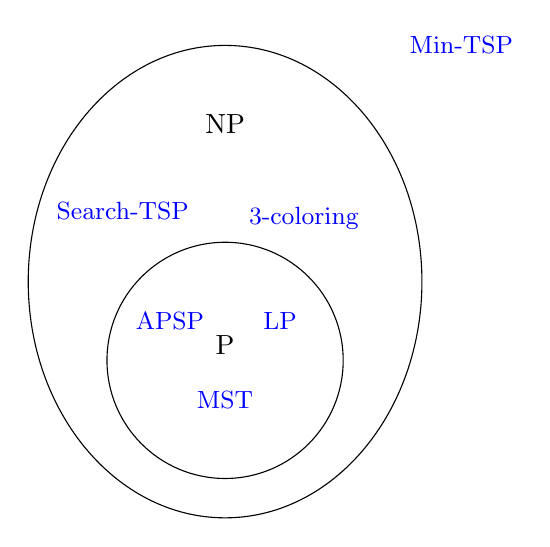
\begin{tikzpicture}
				\draw(0, 0) circle [radius=1.5cm];
				\draw node at (0, 0.2) {P};
				\draw (0, 1) ellipse [x radius = 2.5, y radius = 3];
				\draw node at (0, 3) {NP};
				\draw[blue] node at (0, -0.5) {\small MST};
				\draw[blue] node at (0.7, 0.5) {\small LP};
				\draw[blue] node at (-0.7, 0.5) {\small APSP};
				\draw[blue] node at (1, 1.8) {\small 3-coloring}; 
				\draw[blue] node at (-1.3, 1.9) {\small Search-TSP};
				\draw[blue] node at (3, 4) {\small Min-TSP};
			\end{tikzpicture}
		\end{center}
	\item We're not going to prove this, but it has been shown that factoring reduces to the 3-coloring 
		problem. Similarly, factoring also reduces to the Rudrata Cycle problem. 
	\item It turns out that every problem in NP reduces to Rudrata cycle!
	\item These are the most difficult problems in NP, and it can be shown that every problem in NP reduces 
		to an NP-complete problem
	\item \textbf{NP-Hardness:} A problem \(A\) is NP-hard if every problem \(B\) in NP reduces to \(A\). 
	\item \textbf{NP-Completeness:} A problelm \(A\) is NP-complete if \(A \in \text{NP}\) and \(A\) is 
		NP-hard.
	\item Problems in NP that aren't NP-complete are called an \textbf{NP-intermediate} problem 
	\item \textbf{Fact:} Given two problems that are NP-complete, then \(A \preceq_p B\) and \(B \preceq_p A\). 
		So this means that you can basically think of \(A\) and \(B\) are basically equivalent problems. 

		\question{Is this a biconditional?}

		\answer{No, consider two problems in P: they can be reduced to one another, but they are not 
		in NP.} 
		\begin{itemize}
			\item  There are thousands upon thousands of NP-complete problems, and by notion of reduction, 
				they are (in some sense) the same problem.
			\item This also means that if there exists a polynomial time algorithm for any NP-problem, 
				then this would imply that P = NP.
		\end{itemize}
		\question{How is it that if P = NP then every problem becomes NP-complete?}  
\end{itemize}

\subsection{Proving NP-Completeness}
\begin{itemize}
	\item Cook-Levin Theorem: showed that every problem in NP reduces in polynomial time to a circuit SAT 
		problem.
	\item It can then be shown that circuit-SAT reduces to 3-SAT, making 3-SAT an NP-complete problem. In 
		terms of a diagram:
		\begin{center}
			\begin{tikzpicture}[every text node part/.style={align=center}]
				\foreach \x in {0, 4}
						\draw[-stealth] (\x+0.5, 0) -- (\x+2, 0);
				\draw node at (-1, 0) {Every problem \\ in NP};
				\draw node at (3.25, 0) {Circuit\\SAT};
				\draw node at (7.25, 0) {3-SAT};
				\draw [-stealth] (8, 0) -- (10, 1.5) node[right] {Independent \\ Set};
				\draw [-stealth] (8, -0.2) -- (10, -1.5) node[right] {Rudrata Cycle};
			\end{tikzpicture}
		\end{center}
		\question{Finish this Diagram Later}
	\item To show that a problem is NP-complete, we first show that \(A \in \text{NP}\), then 
		pick some problem \(B\) that is known to be NP-complete and show that \(B \preceq_p A\). 
		
		\question{What if we show that \(A \preceq_p B\)?}

		\answer{We don't need to, since \(A \preceq_p B\) is true already because \(B\) 
		is an NP-complete problem!}
\end{itemize}
\subsection{Circuit SAT}
\begin{itemize}
	\item A Boolean circuit is a directed acyclic graph with:
		\begin{itemize}
			\item Input nodes \(x_1, \dots, x_n\) 
			\item one output node, with an output \(C(x)\)
			\item gates marked OR, AND, NOT: \(\lor, \land, \neg\)
		\end{itemize}
		A possible graph is:
		\begin{center}
			\begin{tikzpicture}
				\node (c) {$\lor$}
					child [stealth-] {node (a) [left] {$\land$}  
					child {node {$x_1 = 1$}}
				}
				child [stealth-] {node {$\land$}
				  child {node (b) {\(x_2 = 1\)} }
				  child {node {\(\neg\)} 
					  child {node {\(x_3 = 1\) }}
					}
				};
			\draw[-stealth] (b) -- (a);
			\draw[-stealth] (c) -- (0, 1) node[above]  {1}; 
			\end{tikzpicture}
		\end{center}	
	\item The input to circuit SAT is a circuit \(C\) with \(n\) inputs and \(m\) referring to the number of 
		gates. We want to output an assignment of \((x_1, \dots x_n)\) such that \(x_i \in \{0, 1\}\) 
		such that \(C(x) = 1\).
	\item By the Cook-Levin theorem, circuit-SAT is NP-complete. As for a bit of intuition on why this is true, 
		you can think of every problem as basically a collection of logical inputs, which basically means 
		that every problem can be reduced to some complex circuit of logical gates.  
\end{itemize}
\subsubsection{3-SAT}
\begin{itemize}
	\item Here, we're given \(n\) Boolean variables \( x_1, \dots, x_n\) such that \(x_i \in \{0, 1\} \), and 
		\(m \le  3\) variable clauses that join the variables together. 
	\item We want to output an assignment of \(x_1, \dots, x_n\) that satisfies all the clauses. 
	\item \textbf{Theorem:} Circuit-SAT reduces to 3-SAT

		\textit{Proof:} Suppose we're given an input to a circuit-SAT problem.
\end{itemize}

	\section{Quantum Computing Platforms}
\begin{itemize}
	\item Trapped ions: qubits are single atoms, but we've removed one of the electrons so they're positively charged.
		We do this so that we have better control over them. This is the platform that's pursued by Honeywell/
		Quantinuum, AQT, among other companies.  

		\textbf{Pros:}
		\begin{itemize}
			\item These have long coherence times \( T_2 \sim 1 \) minute
			\item They operate at room temperature -- basically it's just a big vaccuum chamber sitting in a room 
				without the need for cryogenics. Nothing about the qubits require low temperature, we just happen 
				to involve cryogenics in order to achieve a better vaccuum. 
			\item Highest fidelity gates so far, and have been one of the first to discover quantum gates.  
		\end{itemize}

		\textbf{Cons:}
		\begin{itemize}
			\item Gates operate typically at 50 microseconds.  
			\item Requires lasers, optics
			\item The coulomb interaction between ions makes scaling more difficult
		\end{itemize}
	\item Neutral Ions: basically the same trapping techniques, except the atoms are neutral instead of 
		charged. We can't trap them using fields because they are neutrally charged. 

		\textbf{Pros:}
		\begin{itemize}
			\item Long qubit coherence times
			\item Room temperature operation 
			\item Inherently somewhat scalable, since neutral atoms don't interact
			\item Optical interface. 
		\end{itemize}
		\textbf{Cons:}
		\begin{itemize}
			\item Experiments usually looks like a mess (requires a lots of lasers), and much of the effort goes into 
				managing the lasers
			\item Requires an ultrahigh vaccuum (so we need cryogenics basically)
			\item Trapping is inherently more difficult and requires high laser power 
		\end{itemize}
	\item Superconducting qubits: these are man-made qubits instead of atoms. 

		\textbf{Pros}
		\begin{itemize}
			\item Chip-based architecture. It's something that we can imagine scaling up to a chip, and we interact 
				with it electronically
			\item Fast gate times (on the order of 50 nanoseconds)
			\item Previously leading the field commercially, but starting to recognize that superconducting 
				qubits might not be the way. (some comapnies are starting to invest in atomic-based approaches)  
		\end{itemize}

		\textbf{Cons:}
		\begin{itemize}
			\item Requires dilution refrigerators, so need cryogenic temperatures 
			\item Short coherence times, though this is getting much better 
			\item Control lines needed for every individual qubit -- every single qubit you want to add means an 
				extra set of lines you need to connect to your system. 
			\item Not very anharmonic. 
		\end{itemize}
	\item Quantum Dots: creating a 2D electron gas, and is possibly the most similar to the structure that we studied 
		in the previous lecture. 
		
		\textbf{Pros:}
		\begin{itemize}
			\item Semiconductor chip based architecture
			\item High fidelity, fast-qubit and two qubit gates. 
			\item Controlled by microwaves and electronics, there are no lasers required in this process. 
		\end{itemize}
		
		\textbf{Cons:}
		\begin{itemize}
			\item Requires cryogenic temperatures
			\item Short coherence times 
			\item Lots of tuning required for each device -- very sensitive architecture
			\item Scaling up to many qubits is still an open problem. We can do 2-qubit gates, but it's not clear 
				how we would scale up beyond that. 
		\end{itemize}
	\item Photonics: none of the stuff that we've talked about so far really applies here. States are single 
		photons, where the information is either stored in the polarization or which rail the photon 
		lives on. 
		
		\textbf{Pros:}
		\begin{itemize}
			\item Silicon chip based architecture
			\item Room temperature operation, what this basically means is that in principle we can do this 
				at room temperature, but the best photon detectors still require cryogenics. 
			\item Fairly easy to scale up, since photons naturally fly around
			\item "Measurement" based -- some of the gates are very easy to physically implement. For instance, 
				if you wanted to change the polarization then all you'd do is just introduce a wave plate
		\end{itemize}
		
		\textbf{Cons:}
		\begin{itemize}
			\item Gate operations are very difficult to achieve, and are inherently probabilistic. Preparing 
				the state itself is a challenge (trying again and figuring out when you succeed), then performing 
				the desired computation afterwards. 
			\item Requires identical photonic states and photonic elements
			\item Low gate fidelities
		\end{itemize}
\end{itemize}
\subsection{Trapped Ions}
\begin{itemize}
	\item Ideally we'd like to use the simplest atom possible, which in our case would be hydrogen-like 
		atoms. We can't use hydrogen itself, because transitions for hydrogen are in the UV spectrum, which poses 
		some challenges (what specifically?)
	\item Commercially, we normally use alkaline earth metals and then strip one electron off so that we end up with 
		a hydrogen-like atom. 
	\item Hydrogen-like atoms have a principal quantum number \( n \), whose energy scales with:
		\[
		E_n = -\frac{z^2 \frac{\mu}{m} E_H}{2n^2}
		\] 
		\( E_H \) is a physical constant, which is written as \( E_H = mc^2 \alpha^2 \)
	\item We also have angular momentum \( \ell \), which has possibilties between \( 0 \) to \( n - 1 \). 
	\item Transitions between these obey selection rules, which tells us that \( \Delta \ell = \pm 1 \) and 
		\( \Delta m = \pm 1 \). 
\end{itemize}

	\section{2D Image Processing}
\begin{itemize}
	\item To start, we first characterize an image as a grid with 
		\( M  \) rows and \( N \) columns, which we denote as 
		living in \( \R^{M \times N} \). 
	\item So, a digital image can be represented as a matrix, generally 
		written as \( f[m, n] \in \R^{M \times N} \). The value of the 
		entry can symbolize an intensity (in grayscale).
	\item With color images, you can define them in RGB colors, then this 
		is a \( M \times N \times 3 \) dimensional matrix. Here, 
		each pixel \( f[m, n] \) is represented by a vector 
		\( (r, g, b) \in [0, 1] \), 
	\item Images can also be complex-valued, where each entry \( f[m, n] \) now has a magnitude and phase. 
		 \[
			 f[m, n] = \text{mag}[m, n] e^{i \text{phase}[m, n]}
		\] 
		We can now
		plot two different maps: one that just shows magnitude, and another that shows phase. 
\end{itemize}
\subsection{Sampling}
\begin{itemize}
	\item We can downsample in two different directions:
		\[
			x[m, n] \to x[2m, 3n]
		\] 
		so this means that we down sampled by a factor of 2 in rows and a factor of 3 in columns. So, the number of 
		rows reduces by a factor of 2, and the columns by a factor of 3. This is one way that we can reduce 
		the amount of information contained in an image, so that it may be sent over channels that can't handle 
		that much capacity. 
	\item We can also upsample, in the same way we defined it for one-dimensional signals.
		\[
			x[m, n] = \begin{cases}
				x\left[ \frac{m}{2}, \frac{n}{3} \right] & \text{\( m \) is a multiple of 2 and \( n \) is a multiple of 3}\\
				0 & \text{else}
			\end{cases}
		\] 
		so this is the way we increase the length of the signal, by basically sandwiching zeros between our known 
		values. The strategy to do this is to do the rows first, then do the columns.    
	\item The issue with upsampling is that because we fill in the matrix with zeros, it introduces undesirable 
		lines into the final image, which we can fix using interpolation.   
\end{itemize}
\subsection{Fourier space} 
\begin{itemize}
	\item Recall with discrete 1D sampling that in Fourier space, because upon upsampling we increase the 
		width in time, we decrease the width in frequency. What this means is that over the range 
		\( [-\pi, \pi] \), which is what we originally had, we now will have multiple copies of the 
		original image. 
	\item Then, the way to fix this we pass image through an ideal 2D low-pass filter, which will give us back 
		a single copy of the image. 
	\item We can also realize the same thing in ``time'', by interpolating with a sinc function. \question{Is this 
		convoluiton here?}
\end{itemize}
\subsection{2D Convolution} 
\begin{itemize}
	\item Here, we have a 2D continuous-time signal \( f(x, y) \) and \( g(x, y) \), and convolving them together 
		\( f * * g \):
		\[
		f * * g = \int_{-\infty}^{\infty} \int_{-\infty}^{\infty} f(x', y') g(x - x', y - y') \diff x', \diff y'  
		\] 
		This is exactly the formula that we derived a while back.   
	\item In discrete-time, it's basically the same:
		\[
			f * * g = \sum_{k=-\infty}^{\infty} \sum_{l=-\infty}^{\infty} f[k, l] g[m - k, n - l] 
		\] 
		Here, just like the other case, \( m, n \) is the coordinate, and the summation is over \( k \) and \( l \). 
	\item Visually, there's a couple ways to see what this actually is doing:
		\begin{enumerate}[label=\arabic*.]
			\item Flip the second matrix in two dimensions, shift in 2D, then multiply them element-by-element 
				and sum them together. So, we basically overlay everything on top of each other.  
		\end{enumerate}
\end{itemize}

	\section{Sampling and Streaming}
\subsection{Sampling}
\begin{itemize}
	\item Suppose you have a question you want to ask like ``do you approve of the U.S. Congress?'' that 
		admits a yes (1) or no (0) answer. Our goal is to estimate the fraction of population who say 
		yes.
	\item The naive approach would be to just ask everybody what their opinions are: and we can be certain of 
		our result. 
	\item Instead of doing this, we take a sample population of \( k \) people chosen at random, and collect 
		their answers \( x_!, \dots, x_k \in \{0, 1\}  \), and output the fraction of those that say 
		yes. 
		\[
			\hat p = \frac{1}{k}\sum_{i = 0}^{k}x_i
		\] 
	\item Our goal is to pick \( k \) such that with probability of \( 1 - \delta \), then
		\[
		|\hat{p} - p| \le  \epsilon
		\] 
		where \( p \) denotes the \textbf{true value} of \( \hat{p} \). 
	\item The larger the value of \( k \), the smaller our \( \epsilon \) can be. 
	\item \textbf{Chernoff Bound:} Suppose \( x_1, \dots, x_n \in \{0, 1\}  \) are independent and 
		identically distributed random variables where \( P(x_i = 1) = p\) and \( P(x_{i} = 0) = 1-p \), then 
		\[
			P\left( \left| \frac{1}{k}\sum_{i = 1}^{k} x_i  - p \right| \ge  \epsilon \right) \le 2e^{-2 
			\epsilon^2 k}
		\] 
		\question{How does this relate to the central limit theorem?}
	\item So in order to get \( P(\text{error} \ge  \epsilon) \le  \delta \), then we choose: 
		\[
		k = \left\lceil \frac{1}{2\epsilon^2}\ln\left(\frac{1}{2\delta} \right)\right\rceil 
		\] 
		\comment{There's a mistake in the notes where it says \( \log_2 \), but it should be \( \ln \) instead.} 
\end{itemize}
\subsection{Streaming}
\begin{itemize}
	\item Suppose there's a stream and we're watching fish go by, and we want to know some things about the 
		fish in the stream:
		\begin{itemize}
			\item How many fish went by?
			\item What fraction of fish were red?
			\item How many fish species are there?
		\end{itemize}
	\item The issue is, there are too many fish in the stream to record them all (basically no access to memory).
		Further, we can never rewind the clock: once a fish goes by, it doesn't go by anymore. 
	\item Streaming algorithms are actually used in the real world! (e.g. tracking packets over the internet)
\end{itemize}
\subsection{Sampling from a Stream}
\begin{itemize}
	\item Given a stream \( s_1, \dots, s_i \) (we don't know how many elements there are beforehand), and we want
		to output a uniformly random element from the stream.
	\item One way to do this is to record all elements and output a random \( s_i \). However, this takes 
		up a lot of space and isn't preferred.
	\item If \( L \) (length of stream) is known, then we can pick a random index \( i = \{1, \dots, L\}  \) 
		and output a random \( s_i \). 
	\item Neither of these two models work for our problem, because we don't know \( L \) and the first one 
		is just downright slow.
\end{itemize}
\subsubsection{Reservoir Sampling}
\begin{itemize}
	\item We start with \( r = s_1 \). 
	\item Then, for each new stream element, we flip a biased coin with probability \( p_i = 1/i\) of heads and 
		tails with \( 1 - p_i \). If heads, replace \( r = s_i \). Otherwise, leave \( r \) as is.

		Some intuition on why we might expect \( 1 / i \) : at every step \( i \), we have to handle the case
		 where the stream stops there, in which case we want \( s_i \) to be selected with probability 
		 \( 1 / i \).
	\item When the stream stops, we output \( r \).
	\item This probability is actually uniform! In order to output \( s_i \), then the coin would have 
		flipped heads on element  \( i \), then tails at every \( i \) after that. This happens with probability:
		\[
		P = \frac{1}{i}\left( 1 - \frac{1}{i+1} \right)\left( 1 - \frac{1}{i+2} \right) \dots 
		\left( 1 - \frac{1}{L} \right) = \frac{1}{i} \cdot \frac{i}{i+1} \dots \frac{L-1}{L} = \frac{1}{L}
		\] 
		\comment{Note that the flips before \( i \) don't matter, 
		since if flip \( i \) is heads then \( r \) is replaced anyway.}   
\end{itemize}
\subsubsection{Distinct Elements}
\begin{itemize}
	\item Again, given a stream \( s_i \), we want to estimate the number of distinct elements in the stream. 
	\item To solve this, we pick a random hash function \( h: \{1, \dots, N\}  \to [0, 1] \). As the stream 
		goes by, we compute \( h(s_i) \) for each element. We only keep one value, that value being the minimum
		of \( h(s_i) \), and call it \( \alpha \). Then, when the stream ends, we output \( 1 / \alpha \). 
		
		Intuition for why \( 1 / \alpha \) should be returned: suppose there's \( k \) elements in the stream. 
		As our algorithm goes, then we're only going to see the hash values for those \( k \) elements 
		that have been seen. Call these values \( r_1, \dots, r_k \). Since the hash function is random, we 
		know that they should be (in expectation) evenly distributed on \( [0, 1] \). Therefore, the distance
		between the hash values is  \( \frac{1}{k+1} \) and since \( \alpha \) is the minimum value then 
		\( \alpha = \frac{1}{k+1} \). Therefore, \( \frac{1}{\alpha} = k+1 \), which works as an estimation. 

		\comment{You can subtract 1 off the result, but because we're just estimating it really doesn't matter.} 

		\question{How does the hash function know from \( 1 \) to \( N \)?}  

		\answer{\( N \) is given to you beforehand.}
	\item There are a couple issues with this, mainly that computers can't store arbitrary real numbers, and 
		the hash function takes a lot of memory to store. One solution (preview for next time) is to use a 
		\textit{pseudorandom hash function}.
		\begin{itemize}
			\item One way to circumvent the first problem is to have a hash function  \( h \) map from 
				\( \{1, \dots, R\}  \) where \( R  \) is some very large number. This way,  \( h(i)/R \) is 
				``random enough''.
			\item For the second issue, we make \( h \) a pseudorandom hash function. This takes less space, 
				while still guaranteeing that we get the randomness we want.
		\end{itemize}
\end{itemize}

	\section{Streaming II}
\begin{itemize}
	\item Recall the way we computed the number of distinct elements 
		using a random hash function \( h: \{1, \dots, N\} \to [0, 1] \). 
	\item There were problems with this approach! There were two:
		\begin{itemize}
			\item Computers can't store arbitrarily real numbers

				\textit{Solution:} Pick a hash function that maps \( h: \{1, \dots, R\}  \) instead of 
				\( \{1, \dots, N\}  \) so that \( h(i) / R \) is basically a random number between 0 and 1. This 
				is fairly easy to implement.
			\item If the hash function is uniformly random, then we would require \( N \log R \) bits to 
				store this -- this takes up a lot of memory, especially as \( R \) grows large! 

				\textit{Solution:} Make the hash function \( h \) ``pseudorandom''. We will define 
				a \textit{hash family} \( \mathcal H = \{h_1, \dots, h_m\}  \), and we will choose from this 
				family for our hash function. We will use \( h \sim \mathcal H \) to denote choosing a random 
				\( h_i \). This approach only requires \( \log m \) bits to store, so this is much better
				than our earlier implementation. 

				\comment{Each of \( h_i \) are basically constant functions, we've changed the randomness
				of the hash function to \textit{choosing} the hash function itself.}

				\question{So are the \( h_i \) just random bits, then how are we guaranteeing that we can still 
				get the number of distinct elements?}

				\answer{Just in the same way the hash function expects a spacing of \( \frac{1}{k+1} \), 
				we expect that the randomly generated hash family is also \( \frac{1}{k+1} \).} 
		\end{itemize}
\end{itemize}
\subsection{Pairwise Independence}
\begin{itemize}
	\item This is the way we're going to define randomness.
	\item \textbf{Definition:} A hash family \( \mathcal H = \{h_1, \dots, h_m : \{1, \dots, N\} \to 
		\{1, \dots, R\}	\} \) is \textit{pairwise independent} if:
		\begin{itemize}
			\item For all \( x \neq y \in \{1, \dots, N\}  \) and \( i, j \in \{1, \dots, R\}  \), then 
				\[
					\underset{h\sim \mathcal H}{\mathrm{Pr}}\left[ h(x) = i \text{ and } h(y) = j \right]  
					= \frac{1}{R^2}
				\] 
				where Pr denotes the probability. In other words, it means that our \( i, j \) look like 
				two independent draws from \( \{1, \dots, R\}  \). 
		\end{itemize}
	\item If this is true, it also implies that \( \underset{h \sim \mathcal H}{\mathrm{Pr}}[h(x) = i] =\frac{1}{R} \) for all \( x \) and \( i \).
\end{itemize}
\subsubsection{Generating Pairwise Independence}
\begin{itemize}
	\item Our approach will utilize modular arithmetic, and to make things easy we will do modular arithmetic 
		using a prime \( p \). 
	\item Then, for each \( a, b \in \mathbb{Z}_p = \{0, 1, \dots, p-1\}\), we will define \( h_{a, b}: 
		\mathbb Z_p \to 
		\mathbb Z_p\) such that \( h_{a, b}(x) = ax + b \pmod p\). 
	\item This makes \( \mathcal H = \{h_{a, b}\} _{a, b \in \mathbb Z_p} \) is pairwise independent. Note 
		also that there are \( p^2 \) hash functions, so \( \mathcal H \) takes up \( O(p) \) space.   

		\comment{This is very close to what you'd do with the streaming algorithm, but not exactly.}

		\textit{Proof of Independence (simplified):} Let  \( x, y, i, j \in \mathbb Z_p \) 
		such that \( x \neq y \). We want to show that 
		\[
			\underset{a, b}{\mathrm{Pr}}[ax + b = i \text{ and } ay + b = j] = \frac{1}{p^2}
		\] 
		We will do it for \( x = 0, y = 1 \) and the general case is left as an 
		exercise. In this case, we'd want to prove:
		\[
			\underset{a, b}{\mathrm{Pr}}[b = i \text{ and } a+ b = j] = \frac{1}{p^2}
		\] 
		But given this construction, we know that \( b \) and \( a + b \) is a random pair in \( \mathbb Z_p^2 \),
		so the probability is indeed \( \frac{1}{p^2} \). Note that this is not 3-wise independent: given 
		\( x =0, y = 1, z = 2 \), then \( h(z) = 2a + b = 2(a + b) - b = 2h(1) - h(0) \). Since there's 
		a way to construct \( h(z)  \), this is not independent.
\end{itemize}
\subsection{Modified Distinct Elements}
\begin{itemize}
	\item Instead of throwing our value into a hash function, we will pick a pairwise independent hash 
		function \( h: \{1, \dots, N\}  \to [0, 1] \). 
	\item We compute the \( t \)-th smallest value of \( \{h(s_1), \dots, h(s_L)\}  \), which would be 
		the \( t \)-th smallest value of \( \{r_1, \dots, r_k\}  \). 
	\item Then, we output \( t / \alpha \).
	\item The reason we want to use the \( t \)-th smallest is because want our algorithm to be tolerant to 
		outliers. 

		\question{Why not just use the \( N / 2 \)-th smallest? Shouldn't this be the most tolerant value 
		to outliers?}

		\answer{It is, you can repeat the same analysis for exceedingly large values.} 
\end{itemize}
\subsubsection{Analysis}
\begin{itemize}
	\item We have the property that (based on our algorithm):
		\[
		\mathrm{Pr}[\text{alg outputs} \ge  2k] = \mathrm{Pr}\left[\alpha \le  \frac{t}{2k}\right] = 
		\mathrm{Pr}\left[ \sum_i C(i) \ge  t \right] 
		\] 

		\question{How do we go from the 2nd to the 3rd step?}

		\answer{\( C(i) \) is defined to be the number of outliers, so the probability that we output 
		something larger than \( 2k \) is if there are more than \( t \) outliers.} 

		Here, we define \( C(i)  \) as follows:
		\[
		C(i) = \begin{cases}
			1 & r_i \le  \frac{t}{2k}\\
			0 & \text{otherwise}
		\end{cases}
		\] 
		In other words, \( C(i) \) is an indicator that counts the number of outliers. Then, we have:
		\[
			E\left[ \sum_{i} C(i) \right]  = \sum_{i} E[C(i)] = \sum_i \mathrm{Pr}\left[ r_i\le \frac{t}{2k} \right] = \sum_i \frac{t}{2k} = \frac{t}{2}
		\] 
		Where the second step is reached via linearity of expectation. This means that the expected 
		number of outliers is \( \frac{t}{2} \).

		\question{Is this a good value?}
	\item Now we compute the variance to get a good idea of the spread of \( \sum_i C(i) \):
		\[
			\Var\left[\sum_i C(i)\right] = \sum_i \Var[C(i)] 
		\] 
		Since each \( C(i) \) is associated with an \( r_i \) which is derived from \( h(s_i) \), each 
		\( C(i) \) is also pairwise independent. This allows us to take the summation out of the variance. Then:
		\[
			\Var[C(i)] \le  E[C(i)^2] = E[C(i)] = \frac{t}{2k} \implies \Var\left[ \sum_i C(i) \right] \le k 
			\cdot \frac{t}{2k} = \frac{t}{2}
		\] 
\end{itemize}

	\section{Randomized Algorithms} 
\begin{itemize}
	\item Described as an algorithm which uses random bits to solve problems. Generally, this is done 
		using some function called \( \textsc{RandomInt}(a, b) \) which returns a random integer from 
		the interval \( (a, b) \).
	\item Generally, algorithms will output a \textit{pseudorandom} number (random enough for our purposes) 
		But when we model randomness mathematically, we refer to a genuinely random number.  
	\item Here, algorithms will be allowed to fail with some probability (say 5\%).
	\item Oftentimes, randomized algorithms lead to much more elegant solutions when compared to deterministic 
		algorithms. They can also sometimes be much faster than deterministic ones!
\end{itemize}
\subsection{Background: Integer Factorization}
\begin{itemize}
	\item This is not a problem we know how to solve using a randomized algorithm. Given a number \( N \), 
		we want to find its prime factorization \( N = p_1p_2\cdots p_k \). 
	\item Naively, we could just test every single number from 1 to \( \sqrt{N}  \), but this takes 
		\( O(\sqrt{N} ) \) time (if \( N \sim 10^{500} \), then our algorithm would take longer than the number 
		of atoms in the universe to compute.)
	\item The best algorithm we know today is called a \textit{General Number Field Sieve}, which factors 
		an \( n \) bit number in time \( C^{n^{1 / 3}\log(n)^{2 / 3}} \). (This \( C \) is not very large, but 
		still not small.) 
	\item This is a very important problem! RSA (the company) literally puts out numbers on the internet with 
		cash prizes attached to them if you can factor them. RSA-250 is a 250-digit number, which was 
		recently factored in 2020. RSA-290 has a \$75,000 cash prize attached to it.
	\item \textit{Aside:} this is a problem that is easily solved by quantum computers.  
\end{itemize}
\subsection{Primality Testing}
\begin{itemize}
	\item Given a number \( N \), our only goal is to figure out whether \( N \) is prime or composite. 
	\item This is very similar to the prime factorization problem! We \textit{could} take \( N \) and factor it, 
		but this is obviously very hard. But we can solve this relatively efficiently using randomness!
	\item We use another property of prime numbers: Fermat's little theorem! It says that if \( N \) is prime, 
		then 
		\[
			a^{N-1} \equiv 1 \pmod{N}
		\] 
		for all \( a \in \{1, 2, \dots, N-1\}  \).
	\item So we define a test called \( \textsc{FermatTest}(N) \). It picks a value \( a \in \{1, 2, \dots, 
		N - 1\}  \) uniformly at random. If \( a^{N} \equiv 1 \pmod N \), then we output "prime", otherwise 
		we output "composite". 
		\begin{itemize}
			\item This algorithm will always output "prime" for prime \( N \). For values that are coprime with 
				\( N \), it's harder to see whether they pass \( \textsc{FermatTest} \), and ones that aren't 
				are certainly going to fail \( \textsc{FermatTest} \).
			\item Becuase this test relies pretty heavily on the fact that \( a \) is coprime, our test is only 
				as good as the number of coprime \( a \) that we get. 
			\item \textit{Aside:} There do in fact exist are \textit{composite} numbers that satisfy
				\( a^{N-1} \equiv 1 \pmod N \) for all \( a \) coprime
		to \( N \)! In other words, these numbers will always pass \textsc{FermatTest}. These are called 
		\textit{Carmichael numbers}, but for the purposes of this class, we will pretend like these don't exist.
		\end{itemize}
	\item \textbf{Theorem:} Suppose \( N \) is composite and not carmichael. Then, we have 
		\( P(\textsc{FermatTest}(N) = \text{composite}) \ge 1 / 2 \). 
		
		\textit{Proof:} If the number is not Carmichael, this implies the existence of some coprime \( b \)
		such that \( b^{N - 1} \not \equiv 1 \pmod N \), and thus there is a single \( b \) that fails
		\textsc{FermatTest}. 
		
		\textit{Subclaim:} Suppose some value \( a \) passes \textsc{FermatTest}. Then, \( ab \pmod N\)  will fail
		\textsc{FermatTest}. 

		\textit{Proof:} This is because \( ab \) is no longer coprime to \( N \), so this gives us a 
		1-1 correspondence between a value that passes \textsc{FermatTest} and one that doesn't. More 
		rigorously, we have:
		\begin{align*}
			(ab)^{N - 1} & \equiv a^{N - 1} \cdot b^{N - 1}\pmod N\\
						 &\equiv b^{N - 1} \pmod N\\
						 &\not \equiv 1 \pmod N
		\end{align*}
		where we use the fact that \( a^{N - 1} \equiv 1 \pmod N \). Then, the one-to-one correspondence follows.
		Then, since there are values that \textit{just fail} \textsc{FermatTest}, then this means that 
		there are more values that fail than pass. Hence, \( P(\text{fail}) \ge  1 / 2 \), as desired.   
	\item Now, let's repeat this algorithm \( k \) times. On any given test, we know that if \textsc{FermatTest}
		returns "composite" then \( N \) is definitely composite, so the only case where we get a fail is if 
		\( N \) is composite but \textsc{FermatTest} outputs "prime". This occurs with probability 
		\[
		P(\text{\( N \) composite but outputs prime}) = 1 - \frac{1}{2^{k}}
		\] 
		This means that when our test outputs "prime", there is a \( 1 - \frac{1}{2^{k}} \) chance of it being 
		a false positive. 
	\item We can add another check to detect Carmichael numbers -- we won't really delve into this here. This 
		gives the Miller-Rabin primality test, developed in 1976. 
	\item Since then, there have been improvements: the AKS Primality test (2002) gave a deterministic 
		polynomial time \( O(n^{12}) \) algorithm for primality testing.   
\end{itemize}
\subsection{Randomized Complexity Classes}
\begin{itemize}
	\item Some problems have both efficient randomized and deterministic algorithms, but there are others 
		that only have efficient randomized algorithms. (e.g. polynomial identity testing) 
	\item This implies the existence of two possible worlds:
		\begin{enumerate}[label=\arabic*.]
			\item Every efficient randomized algorithm has a corresponding deterministic solution. (P)
			\item Some problems only have efficient randomized algorithms. (BPP)
		\end{enumerate}
	\item The question of which world we live in is called the P vs. BPP problem. P is the class of efficiently 
		deterministic problems (same P as before), and BPP is the class of efficient, randomized algorithms. We 
		think that these complexity classes are equal. 
\end{itemize}
\subsection{Minimum Cut} 
\begin{itemize}
	\item Consider a (unweighted, undirected) graph \( G = (V, E) \), and we want to find the minimum cut of this graph. Here, 
		the heuristic we're using to quantify the size of the cut is the number of edges it crosses through.
	\item Recall from our max-flow problem, we found the minimum \( s-t \) cut via our flow algorithm. It turns out that 
		 we can use the flow algorithm to solve this deterministically via a reduction, but today we'll talk about another 
		 algorithm: Karger's algorithm. 
	 \item For every \( i = 1, \dots, n- 1 \), it will:
		 \begin{enumerate}[label=\arabic*)]
		 	\item Pick a uniformly random edge \( e \), and "contract" the edge.
			\item It will return the cut specified by the remaining two supervertices.  
		 \end{enumerate}
	 \item The way to contract an edge is to combine the two vertices connected by \( e \), and combine them into one supervertex.
		 It will preserve all the possible edges, which means that the graph doesn't have to remain simple in this process.  
		 Then, once only two vertices are remaining, then that's the cut that we output. Notice that because we don't delete any
		 edges in this process, then the size of the "supercut" is equal to the size of the cut in the original graph. 
	 \item This won't return the minimum cut, but it will return the minimum cut with fairly good probability.  
\end{itemize}
\subsubsection{Intuition}
\begin{itemize}
	\item So suppose we have a graph with a bunch of edges, then with one singular edge outside, like this:
		% add a figure here
	\item If Karger's algorithm is to find the minimum cut, then it should never contract edge \( e \). Basically, it leverages
		 the fact that becuase there are more edges outside of the minimum cut, then the algorithm shouldn't select the edges 
		 along the minimum cut. 
	 \item \textbf{Theorem:} Let  \( C = (S, \overline S) \) be a minimum cut of size \( k \). Then, the probability that 
		 Karger's algorithm outputs the cut \( C \) is given by:
		 \[
			 P(\text{Karger's outputs \( C \)}) \ge \frac{1}{{n \choose 2}} = \frac{2}{n(n-1)}
		 \] 
		 While this is indeed bad for a single iteration, it just means that in expectation we just need to repeat this 
		 \( n^2 \) times to get the minimum cut!
	 \item \textit{Proof:} First, we state four facts:
		 \begin{itemize}
		 	\item Let \( G_i \) be the state of the graph \( G \) at the \textit{start of the} \( i \)-th iteration. Then, because 
		 \( C \) is the minimum cut with size \( k \), then we know that the minimum cut of \( G_i \ge k \). 
			\item Further, the number of vertices in \( G_i  \) is \( n - (i - 1) = n-i+1\). 
			\item The degree of each vertex in \( G_i \ge  k \), because of the fact that the minimum cut is \( k \). Had 
				the degree been less than \( k \), then the minimum cut would be less than \( k \), since the min-cut 
				would just be to cut that vertex with degree less than \( k \). 
			\item The number of edges in \( G \) can be calculated as:
				\begin{align*}
					N &= \frac{1}{2}\sum_{v \in G_i} \deg(v)\\
					  &\ge \frac{1}{2}\sum_{v \in G_i} k\\
					  &= \frac{1}{2}k |G_i| \\
					  &= \frac{1}{2}k(n-i+1) 
				\end{align*}
		 \end{itemize}
		 Now we complete the proof. Essentially, we want to compute the probability that the algorithm never contracts a cut 
		 in \( C \). Suppose at step \( G_i \), we haven't contracted any edges in \( C \). Then, the probability 
		 that we don't contract an edge in \( C \) is:
		 \[
		 	P(\text{don't contract an edge in \( C \)} = 1-P(\text{contract an edge in \( C \)}) 
			= 1 - \frac{k}{\frac{1}{2}k (n - i + 1)}
		\]
		Thus, the probability that we never contract an edge in \( C \) is the probability that this event occurs on every 
		iteration \( i \), at the step \( G_{i - k} \) :
		\[
		P(\text{never contract edge in  \( C \)}) \ge  \left( 1 - \frac{2}{n} \right) \left( 1 - \frac{2}{n-1} \right) \dots 
		= \frac{2}{n(n-1)}
		\] 
		So therefore, the probability that we succeed is lower bounded by \( \frac{2}{n^2} \).
\end{itemize}
	\section{Quantum Algorithms}
\subsection{Brief History}
\begin{itemize}
	\item In the world of physics, there was a problem: we couldn't simulate quantum systems. What does that even mean?
	\item Suppose we have \( n \) electrons, each with spin \( \ket{\uparrow} \) or \( \ket{\downarrow} \). 
		This gives us a total of \( 2^{n} \) possible configurations. The fastest algorithm known at the time 
		was one that took \( O(2^{n}) \) time.
	\item Richard Feynman suggested in a 1981 talk that we could potentially build a computer out of 
		electrons, and instead of computing the quantum mechanics itself, we just let the electrons 
		simulate themselves.
	\item How powerful are quantum computers actually? Very powerful! A small list of algorithms that 
		are very powerful:
		\begin{itemize}
			\item Deutsch-Jozsa algorithm: solves the Deutsch-Josza problem
			\item Bernstein-Vazirani algorithm
			\item Simon's algorithm
			\item Shor's algorithm
			\item Grover's algorithm
		\end{itemize}
\end{itemize}
\subsection{Deutsch-Josza Problem}
\begin{itemize}
	\item Given an input function \( f: \{0, 1\} ^{n} \to [0, 1] \), the function is one of the following:
		\begin{enumerate}[label=\roman*)]
			\item \( f(x) = 0 \) for all \( x \) 
			\item \( f(x) = 1 \) for all \( x \) 
			\item \( f(x) = 0 \) for half of \( x \), and \( f(x) = 1 \) for the other half. 
		\end{enumerate}
	\item We proved that classical deterministic algorithms have to check at least \( 2^{n-1} +1 \) values 
		for \( f(x) \) to determine. This means that the algorithm runs in exponential time. However, 
		the quantum algorithm can do this process in \( O(n) \) time!
	\item There is also a very simple randomized algorithm for this: we can pick a subset of \( x \) at random,
		and this allows us to determine the identity of \( f(x) \) also fairly quickly.
	\item So this problem tells us the power of quantum computers over deterministic algorithms, but doesn't 
		show the power of quantum algorithms over random algorithms. 
\end{itemize}
\subsection{Bernstein-Vazirani Problem}
\begin{itemize}
	\item Given an input function \( f: \{0, 1\} ^{n} \to \{0, 1\}  \) that takes a subset of \( x \) and 
		adds the values up modulo 2, we want to figure out which bits were added in the sum.  
	\item Classically, we can look at all the possible configurations for \( f \), which would require 
		\( n+1 \) looks at \( f \). However, the quantum algorithm only needs to look at \( f \) once!
\end{itemize}
\subsection{Shor's Algorithm}
\begin{itemize}
	\item We know that if we have an \( n \)-digit number, the best classical algorithm factorizes a number in 
		\( O(e^{1.9 n^{1 / 3} \cdot \log(n)^{2 / 3}}) \), but Shor showed that we can factor numbers 
		in \( O(n^2) \) time on a quantum computer. 
	\item This is significant, because RSA encryption relies factoring large numbers and this algorithm basically 
		gives us a way to break that encryption scheme. 
\end{itemize}
\subsection{Grover's Algorithm}
\begin{itemize}
	\item This algorithm solves circuit-SAT in \( O(\sqrt{2} ^{n}) \) time on a quantum computer, wherea s
		a classical algorithm takes \( O(2^{n}) \) time. This also solves many other problems (just due to their 
		relationship to circuit-SAT).
\end{itemize}
\subsection{Speedups}
\begin{itemize}
	\item There are three main types of speedups:
		\begin{itemize}
			\item Shor-Type: these are exponentially faster than classical algorithms, but only work on 
				a very restricted subset of problems.
			\item Grover-Type: This speeds up things polynomially, but with the benefit that they work on a large
				number of problems. 
			\item Physics Simulation: Exponentially faster, but can only work for physics problems. 
		\end{itemize}
	\item One of the main reasons why quantum computers outperform classical ones is mainly because they can 
		compute very fast Fourier transforms, which are used everywhere in computation.  
	\item However, quantum computers are not able to solve NP-complete problems efficiently. 
\end{itemize}

\end{document}
